\documentclass[paper=a4, parskip, numbers=noenddot, toc=listof, headsepline]{scrbook}

\usepackage[hang]{caption}
\usepackage{subcaption}
\usepackage{microtype, textcomp}
\usepackage{longtable}
\usepackage[intlimits]{mathtools}
\usepackage{amsfonts, amssymb, array, tabularx, scrlayer-scrpage, multirow}
\usepackage{fontspec}
\usepackage{unicode-math, icomma}
\usepackage{polyglossia}
\setdefaultlanguage[spelling=new]{german}
\usepackage[autostyle]{csquotes}
\usepackage[per-mode=fraction, locale=DE, detect-all=true]{siunitx}
\usepackage[scale=.73]{geometry}
\usepackage{graphicx}
\usepackage{datetime}
\usepackage[backend=biber, isbn=false, doi=false, eprint=false, url=true, safeinputenc, defernumbers=false]{biblatex}
\usepackage[unicode=true, colorlinks=false, breaklinks=true, pdfborder={0 0 0}]{hyperref}
\usepackage{bookmark}

\newcommand{\origttfamily}{}
\let\origttfamily=\ttfamily
\renewcommand{\ttfamily}{\origttfamily \hyphenchar\font=`\-}
\defaultfontfeatures{Ligatures=TeX}
\renewcommand{\dateseparator}{.}
\renewcommand\tabularxcolumn[1]{p{#1}}

\setmainfont{Tex Gyre Termes}
\setmathfont{Tex Gyre Termes Math}
\setsansfont{Latin Modern Sans}[Scale=MatchLowercase]
\setmonofont{LMMonoLt10-Bold}[Scale=MatchLowercase]


\newcommand{\pic}{\emph{Pyro Ignition Control}}
\newcommand{\anlage}{\emph{El Fueradoro}}


%% Seitenstil-Einstellung
\renewcommand{\chapterpagestyle}{plain}
\pagestyle{scrheadings}
\renewcommand*{\partmarkformat}{}
\automark[part]{part}
\clearscrheadings
\clearscrplain
\ohead[\pagemark]{\pagemark}
\lohead[]{\textnormal\headmark}
\rehead[]{\anlage}

\hyphenation{Putty-tel}

\setuptoc{toc}{totoc}

\hypersetup{pdfinfo={
		Title=\anlage,
		Author=Felix Pflaum,
		Subject={User manual for remotely controlled firework ignition system},
		Keywords={}}
}

\usepackage{remreset}
\makeatletter
\@removefromreset{footnote}{part}
\@removefromreset{footnote}{chapter}
\makeatother

\DeclareSIUnit{\dBm}{dBm}

\begin{document}
	\begin{titlepage}
		\thispagestyle{empty}
		{\sffamily\LARGE Benutzerhandbuch{\hfill}Dokumentation{\hfill}Aufbauanleitung}\\ \hrule \vspace*{\fill}
		\begin{center}{\fontsize{90pt}{90pt} \sffamily\textbf{\anlage}} \\ \vspace{2em}
			{\LARGE \sffamily Funkgesteuertes Zündsystem für Feuerwerke}
		\end{center}
		\vspace*{\fill}
		\hrule
		\begin{center}
			\sffamily\Large Felix Pflaum (\href{mailto:f.pflaum@gmail.com}{f.pflaum@gmail.com})\\
			\normalsize \ddmmyyyydate\today, \currenttime
		\end{center}
	\end{titlepage}
	%
	\chapter*{Wichtige Hinweise}
		\addcontentsline{toc}{chapter}{Wichtige Hinweise}

		Vor Inbetriebnahme sollte in jedem Fall diese Anleitung gelesen und verstanden werden! Speziell die folgenden, weiter hinten in der Anleitung detaillierter ausgeführten Hinweise müssen beachtet werden, um Personenschäden oder Beschädigungen an den Geräten zu vermeiden:

		{\bfseries
		\begin{enumerate}
			\item Bei den Zündboxen der ersten Generation liegt das Metallgehäuse des SMA-Antennen\-anschlusses an der Oberseite der Zündbox auf Massepotential, die roten Anschlussklemmen nach dem Einschalten und unter Umständen auch noch Minuten nach dem Ausschalten bei \SI{22,5}{\volt}. Ein Kurzschluss zwischen diesen beiden Punkten ist daher unbedingt zu vermeiden, um Schäden an der Schaltung und ungewollte Zündungen zu verhindern. Daher, sofern der Antennenanschluss nicht isoliert ist, beim Anschließen die Anzünder immer zuerst mit der schwarzen Klemme, danach mit der roten verbinden, beim Abklemmen zuerst das Kabel an der roten, dann das an der schwarzen Klemme lösen. Weiterhin sollte man die Zündbox erst in ihrer endgültigen Position einschalten, so dass ein unbeabsichtigtes Herausziehen der Kabel tunlichst ausgeschlossen ist. Sicherheitshalber kann auch der SMA-Stecker nach dem Anschrauben mit Klebeband isoliert werden. Bei den Zündboxen der zweiten Generation sind schaltungstechnische Maßnahmen getroffen, um den Strom im Kurzschlussfall zu begrenzen und ein Auslösen der Anzünder bei Verbindung zwischen roter Klemme und Antennenanschluss im nicht-scharfgeschalteten Zustand auszuschließen.
			\item Devices nie ohne angeschlossene Antenne einschalten, um Rückreflexionen an offenen Steckern/Buchsen zu vermeiden, welche die Sendeendstufe zerstören könnten.
			\item Keine Softwareupdates an Zündboxen durchführen, solange Anzünder angeschlossen sind, da das Verhalten nach einem fehlgeschlagenen Update unvorhersehbar ist.
		\end{enumerate}
		}

		Trotz aller Sorgfalt bei der Entwicklung von Hard- und Software sowie ausgiebigen Tests seitens der Entwickler kann keinerlei Garantie für Sicherheit und Funktionalität von {\anlage} sowie keine Haftung für Sach- und Personenschäden, welche sich direkt oder indirekt aus dem Einsatz von {\anlage} ergeben, übernommen werden. Es werden mit {\anlage} dem Anwender lediglich Schaltpläne, Layouts und Programmcode sowie Hinweise zu Aufbau und Verwendung einer elektronischen Funkzündanlage, welche er frei weiter verbreiten und~-- selbstverständlich auf eigene Gefahr~-- verändern darf, zur Verfügung gestellt. {\anlage} ist und bleibt ein Hobby-Bastelprojekt, kein geprüftes oder in irgendeiner Form zertifiziertes Produkt!

		Der Umgang mit Feuerwerkskörpern und explosivem Material unterliegt in Deutschland gesetzlichen Restriktionen, deren Einhaltung im Verantwortungsbereich des Anwenders liegt. {\anlage} darf nicht von Personen unter 18 Jahren bedient werden.
		%

		\tableofcontents
		%
	\part{Benutzerhandbuch}

		\chapter{Das System}

				{\anlage} ist eine Eigenentwicklung zur automatisierten Zündung von Feuer\-werks\-choreo\-gra\-phien per Computer und Funk, der Name {\anlage} leitet sich als Kofferwort aus den spanischen Wörtern \emph{fuego}, \emph{radio} und \emph{oro} her und bedeutet frei übersetzt daher so etwas wie \enquote{Goldenes Funkfeuer}. Sie wurde zur Verwendung mit der frei verfügbaren Software {\pic} von Yannic Wilkening (Version 1.4.5) geplant.

			Es besteht aus einer mit dem PC verbundene Transmitterbox, welche die von {\pic} generierten Zündbefehle per Funk an die Zündboxen weitergibt und einer oder mehreren Zündboxen mit je 16 Kanälen zur elektrischen Zündung. Der klassische Aufbau des Systems ist schematisch in Abbildung~\ref{fig:system} gezeigt. Die reine Transmitterbox wird nicht zwingend benötigt; es kann alternativ auch eine Zündbox per Kabel mit dem PC verbunden werden und neben ihrer originären Aufgabe auch die Transmitteraufgaben bewältigen.

			\begin{figure}
				\centering
				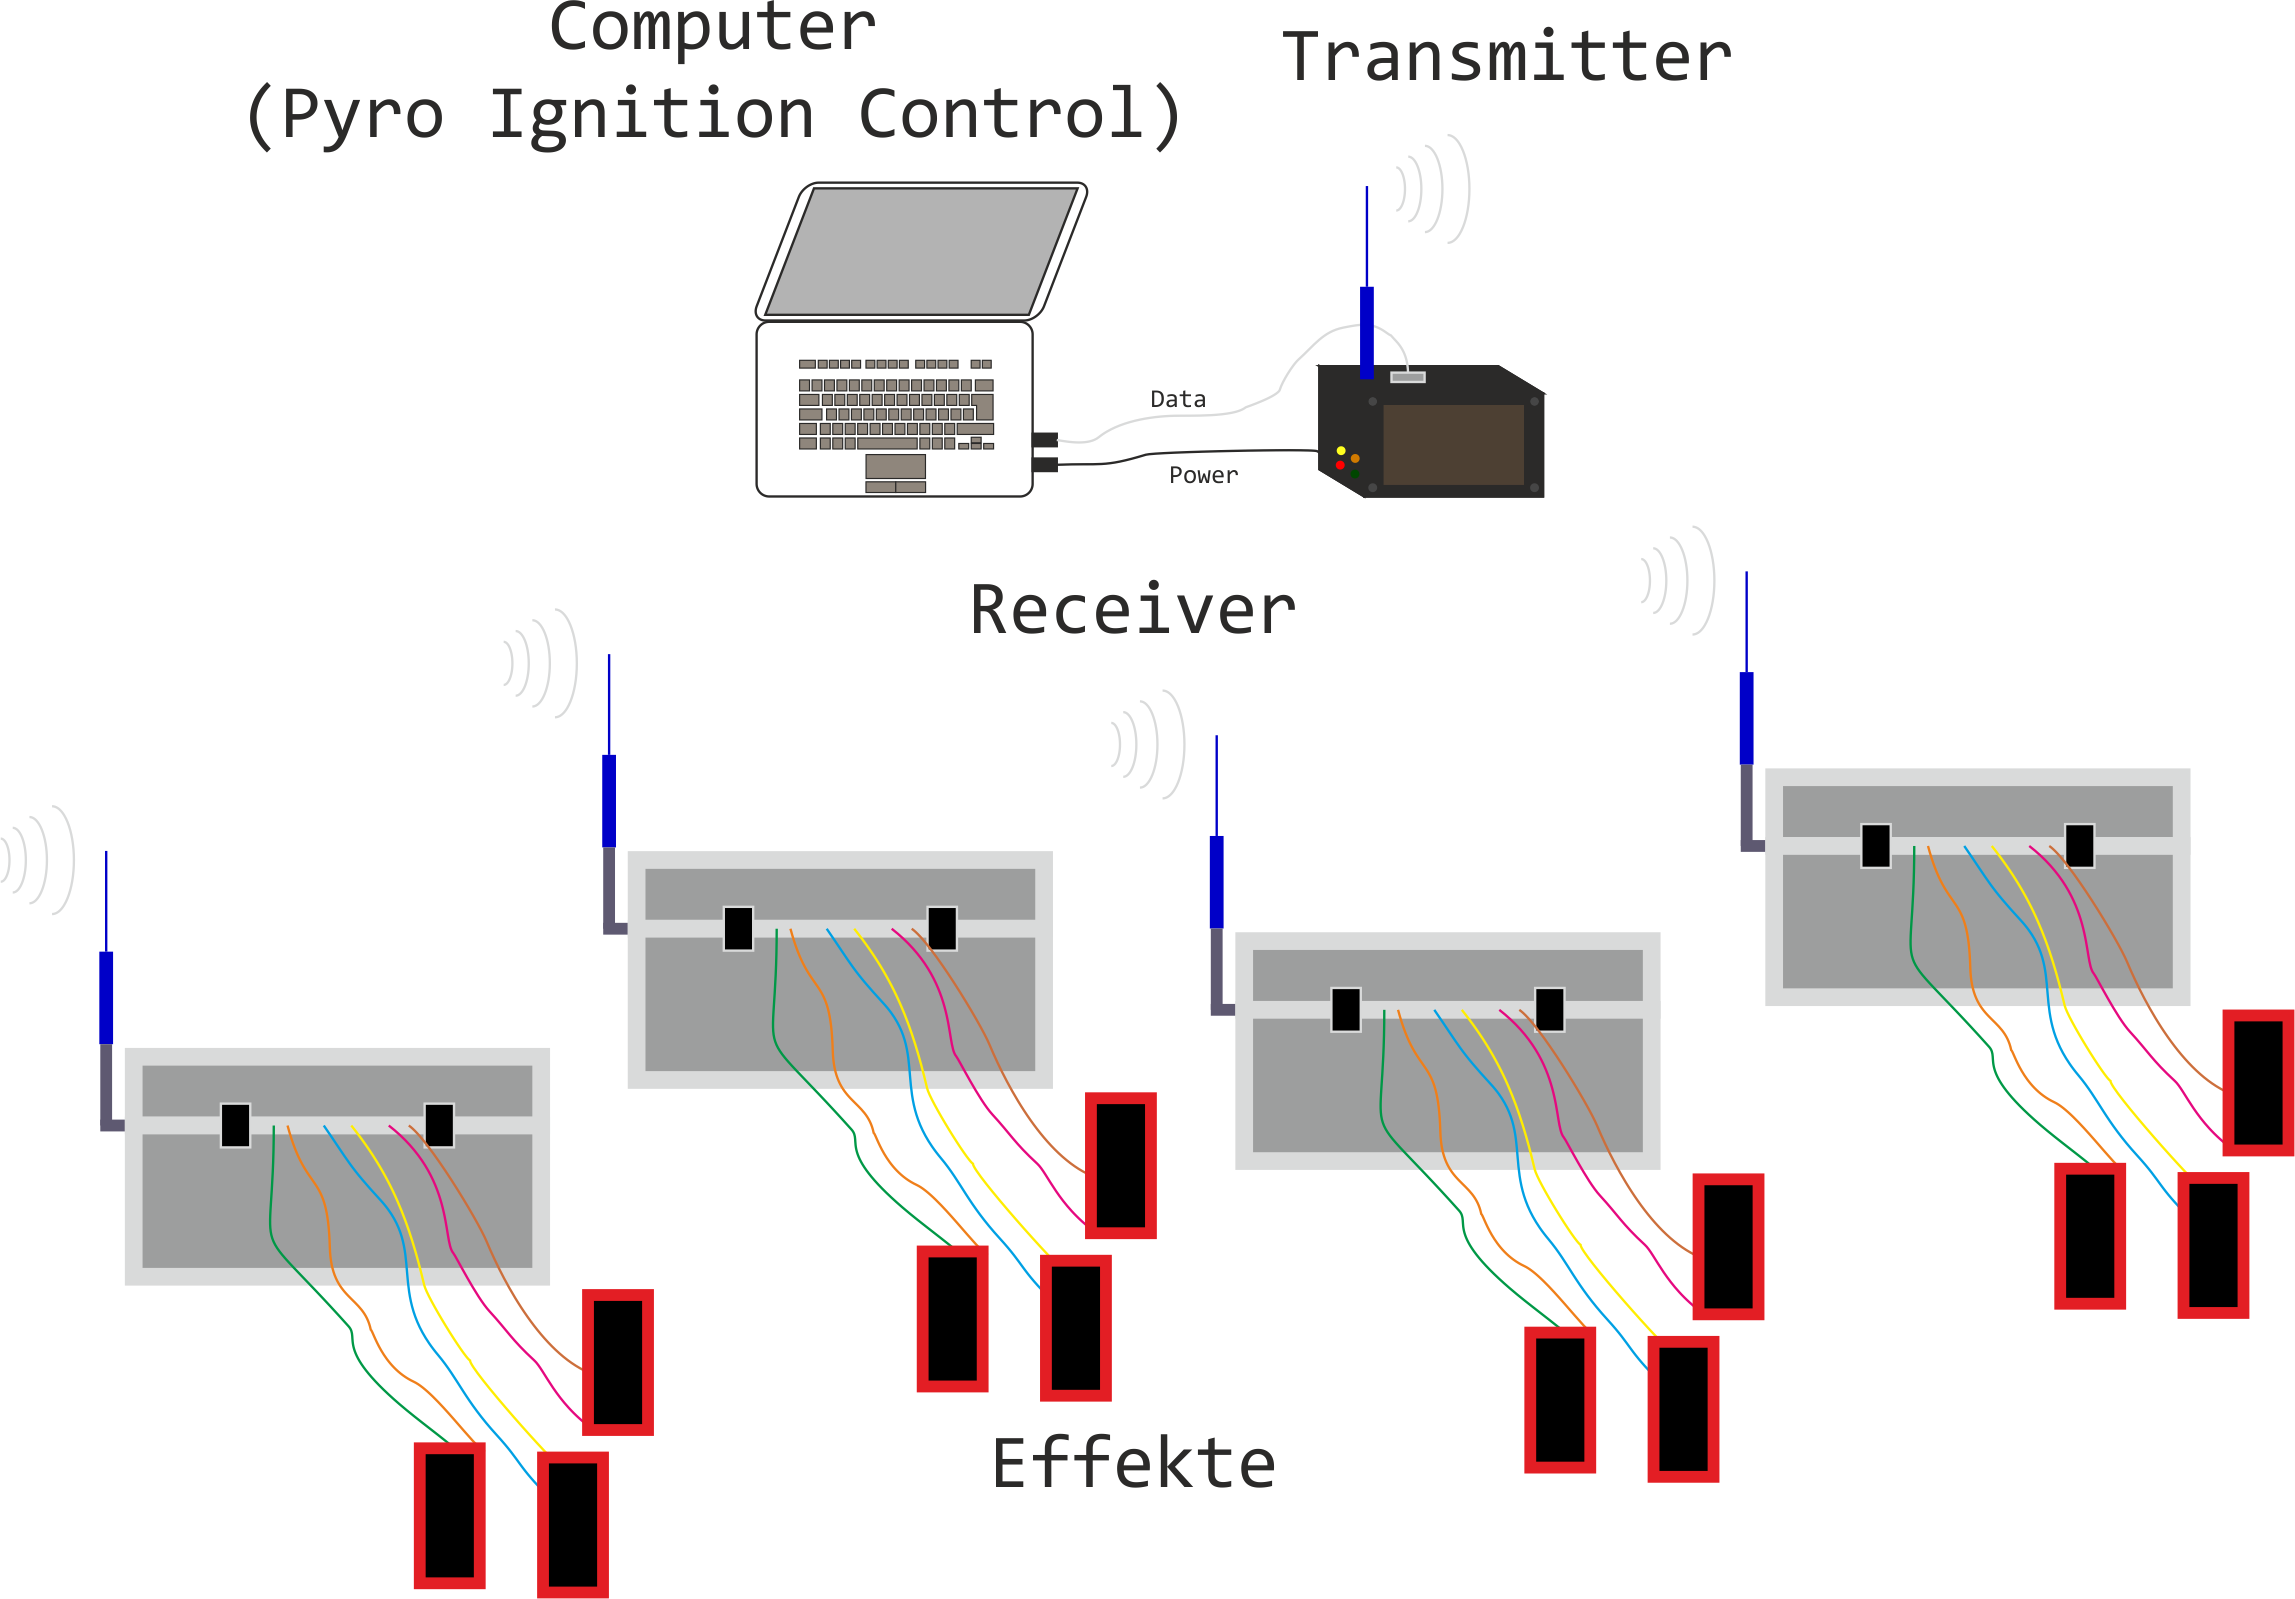
\includegraphics[width=.8\textwidth]{Bilder/system}
				\caption{Systemübersicht \anlage}
				\label{fig:system}
			\end{figure}

			Um möglichst große Flexibilität bei der Gestaltung eines Feuerwerks mit {\anlage} zu gewährleisten, was z.\,B. die Anzahl der verwendeten Zündboxen oder auch die Tatsache angeht, dass man identische Effekte gerne zeitgleich an zwei weiter voneinander entfernten Orten zünden möchte, können den Boxen per Software zwei Kennnummern (Unique-ID und Slave-ID) zugewiesen werden. Genaueres dazu findet sich im Abschnitt~\ref{ch:kommunikationpc}.

			Transmitterbox und Zündbox sind in Abbildung~\ref{fig:transmitter} bzw.~\ref{fig:zuendbox} mit ihren wesentlichen Bestandteilen gezeigt. Sie werden im weiteren Text unter dem Begriff \enquote{Devices} zusammengefasst, falls sich Aussagen auf beide Teile beziehen, und in den folgenden Kapiteln näher beschrieben.

			\section{Aufbau}

				Detailliertere Infos zum Aufbau erhalten interessierte Leser in den nächsten Teilen dieses Dokuments ab Seite~\pageref{part:dokumentation}. An dieser Stelle soll nur kurz auf die Funktionalität eingegangen werden. Herzstück aller Devices ist der 8-bit-Mikrocontroller \texttt{ATmega328P} von Atmel, welcher die verschiedenen Peripheriebausteine kontrolliert. In jedem Device befinden sich ein Funkmodul \texttt{RFM69CW} von HopeRF, welches die drahtlose Kommunikation zwischen den einzelnen Devices übernimmt, ein RS232-Treiberbaustein \texttt{MAX202} mit an die Gehäuseaußenseite geführter Sub-D-Buchse zur Kommunikation zwischen Mikrocontroller und PC sowie vier Status-LEDs.

				Die Transmitterbox ist mit einem LC-Display mit 20 Spalten und 4 Zeilen ausgestattet.

				In den Zündboxen befinden sich zwei vom Mikrocontroller gesteuerte kaskadierte Schieberegister \texttt{74HC595}, welche mit ihren insgesamt 16 Ausgängen 16 Feldeffekttransistoren vom Typ \texttt{IRF3708} für die Zündung ansteuern, außerdem ist auf der Platine mit dem \texttt{MC33063} bzw. einem fertigen Modul mit dem \texttt{XL6009} ein Hochsetzsteller zur Erzeugung einer höheren Zündspannung integriert sowie ein Schlüsselschalter zum Scharfschalten der Boxen. Parallel zur Drain-Source-Strecke jedes Feldeffekttransistors ist eine LED mit Vorwiderstand geschaltet, um zu signalisieren, an welchen Kanälen Anzünder angeschlossen sind.

			\section{Transmitter und Zündboxen}

				\begin{figure}
					\centering
					\begin{subfigure}[t]{0.405\textwidth}
						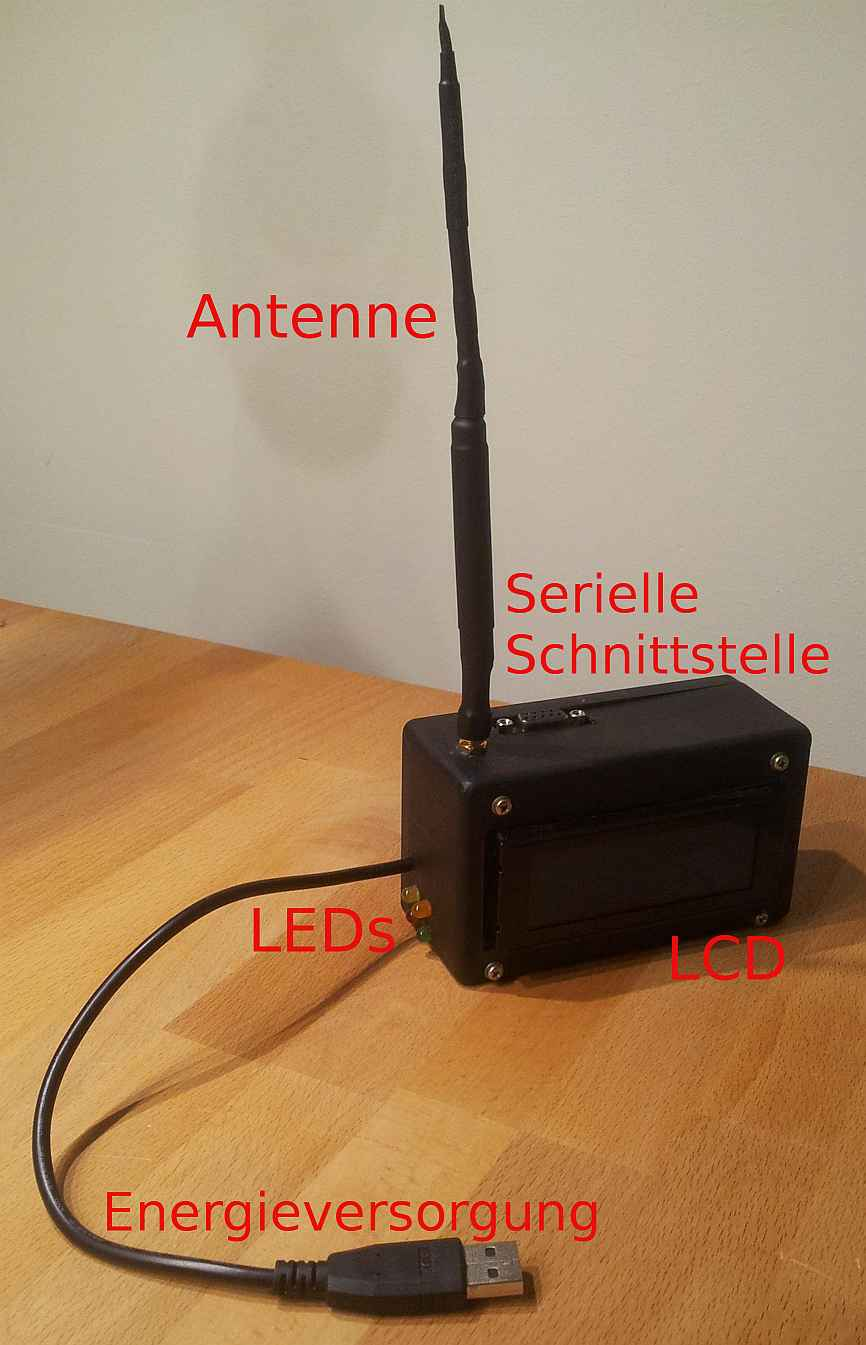
\includegraphics[height=96mm]{Bilder/Transmitter}
						\caption{Transmitter}
						\label{fig:transmitter}
					\end{subfigure}
					\begin{subfigure}[t]{0.55\textwidth}
						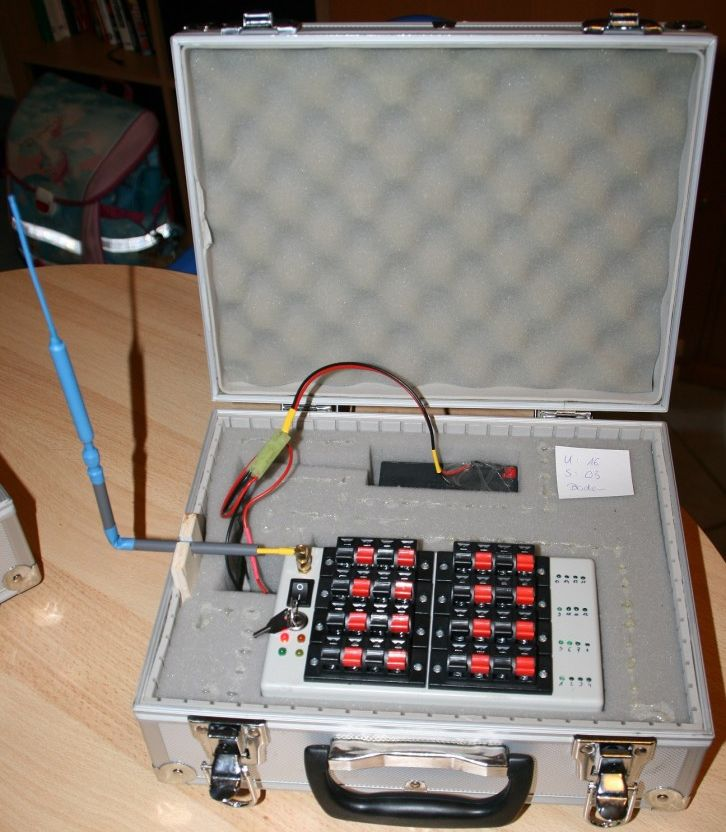
\includegraphics[height=96mm]{Bilder/DraufsichtZuendbox}
						\caption{Zündbox von oben, eingebettet in Koffer}
						\label{fig:zuendbox}
					\end{subfigure}
					%
					\caption{Die Devices von {\anlage}}
				\end{figure}

				Die in Abbildung~\ref{fig:transmitter} gezeigte Transmitterbox dient dazu, die Zündbefehle des PCs per Funk an die über das Gelände verteilt stehenden Zündboxen weiterzuleiten sowie das komplette Funksystem zu überwachen. Hierzu ist im Inneren der Transmitterbox sowie der Zündboxen ein Funkmodul für das~-- im Rahmen der Vorschriften der jeweiligen nationalen Aufsichtsbehörde, in Deutschland der Bundesnetzagentur~-- frei nutzbare Frequenzband um $\SI{868}{\mega\hertz}$ verbaut. Die Datenübertragung vom PC geschieht über eine serielle Schnittstelle.

				Die Zündboxen, in Abbildung~\ref{fig:zuendbox} dargestellt, empfangen die Anweisungen und zünden die einzelnen Kanäle. Jede Zündbox verfügt über 16 einzeln ansteuerbare Zündkanäle. Jeweils eine rote und eine schwarze Klemme bilden zusammen einen Zündkanal, die Nummerierung beginnt links unten mit Kanal 1 und endet rechts oben mit Kanal 16. Alle roten Klemmen sind nach dem Einschalten unmittelbar mit einer Gleichspannung von $\SI{22,5}{\volt}$ verbunden, die schwarzen Klemmen mit dem Drain-Anschluss eines von 16~n-Kanal-MOSFETs.

				Welches der beiden Kabel an welcher Klemme des Zündkanals angeschlossen wird, spielt keine Rolle, da es sich bei den Anzündern um passive elektrische Bauelemente handelt, die in beiden Richtungen gleichermaßen von Strom durchflossen werden können. Die Verdrahtung sollte aber stets im ausgeschalteten Zustand der Boxen erfolgen und aus Sicherheitsgründen immer in folgender Reihenfolge:
				\begin{itemize}
					\item Beim Anklemmen der Kabel zuerst ein Kabel an der schwarzen Klemme befestigen, anschließend das andere an der roten!
					\item Beim Lösen der Kabel zuerst das Kabel von der roten Klemme lösen, anschließend das von der schwarzen!
				\end{itemize}
				Dies ist der Tatsache geschuldet, dass bei der ersten Generation der Zündboxen, wenn eine Seite des Zündkanals fest mit der Zündspannung, d.\,h. einer roten Klemme verbunden ist, ein frei baumelndes zweites Kabel durch Berührung eines Bauteils auf Massepotential, z.\,B. der Antennenbuchse oder der Überwurfmutter des gewinkelten SMA-Steckers, einen Kurzschluss und somit eine Zündung auslösen würde~-- selbst dann, wenn die Box nicht scharf geschaltet ist! In der zweiten Generation der Zündboxen ist dieses Manko behoben.

				Parallel zur üblicherweise sperrenden Drain-Source-Strecke jedes MOSFETs ist eine grüne LED mit Vorwiderstand geschaltet, welcher den Strom durch den LED-Zweig auf unter \SI{5}{\milli\ampere} begrenzt, so dass ein Zünden über die LED ausgeschlossen ist. Sobald die zugehörige schwarze Klemme mit einer roten Klemme~-- die Zuordnung kann beliebig erfolgen, obwohl zwecks Übersichtlichkeit natürlich ratsam ist, die nebeneinander liegenden Klemmen zu nutzen~-- verbunden ist, also ein geschlossener Strompfad von $\SI{22,5}{\volt}$ zur Schaltungsmasse besteht, wird dies durch Leuchten der zur schwarzen Klemme gehörigen grünen LED signalisiert. Ein Leuchten der grünen LED ist dabei lediglich ein Indikator, dass \enquote{etwas} am jeweiligen Kanal angeschlossen ist, eine Aussage, ob der Widerstand des angeschlossenen Anzündernetzwerks gering genug ist, um eine Zündung auszulösen, wird durch die LED ausdrücklich nicht getroffen.

			\section{Energieversorgung}

				Die in unmittelbarer Nähe des zu steuernden PCs platzierte Transmitterbox bezieht ihre nötige elektrische Energie aus dem USB-Port eines PCs. Das fest mit der Transmitterbox verbundene USB-Kabel dient ausschließlich diesem Zweck. Sie verfügt über keinen Ein/Aus-Schalter, sondern ist eingeschaltet, solange sie mit dem USB-Port verbunden und der PC eingeschaltet ist. Da der USB-Port \enquote{angezapft} wird, ohne in der sonst üblichen Weise mit dem Controller zu kommunizieren, empfiehlt sich, die USB-Verbindung erst nach komplett abgeschlossenem Bootvorgang herzustellen und vor dem Herunterfahren des Rechners wieder zu trennen.

				Aufgrund der anzunehmenden Platzierung der Zündboxen im freien Feld, abseits von Steckdosen und anderen Energiequellen werden sie über eine Batterie versorgt. \textbf{Um ordnungsgemäße Funktionalität zu garantieren und Schäden an der Schaltung zu vermeiden, muss die Batteriespannung zwischen \SI{8}{\volt} und \SI{15}{\volt} liegen!} Empfohlen wird die Verwendung eines Blei-Vlies-Akkus mit Nennspannung \SI{12}{\volt}, wie er auch in Abbildung~\ref{fig:zuendbox} über der Zündbox zu erahnen ist.

			\section{Die Status-LEDs}
				\label{ch:leds}

				Alle Devices verfügen über vier Status-LEDs. Bei den Transmitterboxen liegen sie direkt neben dem Kabel für die Energieversorgung auf der Seite, bei den Zündboxen auf der Oberseite. Diese sind mit ihrer Bedeutung in Tabelle~\ref{tab:statusleds} aufgeführt und leuchten, wenn das jeweilige Device die mit der LED verknüpfte Tätigkeit ausführt.

				\begin{table}
					\centering
					\begin{tabularx}{.7\textwidth}{Xl}
						\hline\hline
						\textbf{Farbe} & \textbf{Funktion}                           \\ \hline
						orange         & Funkmodul empfängt                          \\
						grün           & Funkmodul sendet                            \\
						gelb           & Daten kommen über serielle Schnittstelle an \\
						rot            & Device ist scharf geschaltet                \\ \hline\hline
					\end{tabularx}
					\caption{Farben und Funktionen der Status-LEDs}
					\label{tab:statusleds}
				\end{table}

				Während des Bootvorgangs leuchten bei den Zündboxen die orange und gelbe LED im Wechsel, wodurch dem Benutzer die aktuell eingestellte Slave-ID der Box visualisiert wird. Das nach kurzer Pause folgende Blinken der grünen LED signalisiert dann die Statusmeldung per Funk an allen anderen Devices.

				Bei einem Zündvorgang leuchten an der Zündbox für die Dauer der Zündung (\SI{11}{\milli\second}) alle vier LEDs.

			\section{Das LCD des Transmitters}

				Aktuelle Statusanzeigen werden bei dem Transmitter auf dem LC-Display ausgegeben. Ein Beispiel zeigt Abbildung~\ref{fig:senderanzeige}. In Zeile 1 wird hinter der Abkürzung \enquote{Tx} (Transmitted) der letzte gesendete Befehl angezeigt, in Zeile 2~-- im Bild nicht zu sehen~-- ggf. hinter der Abkürzung \enquote{Rx} (Received) die letzte empfangene Rückmeldung (angeforderte Parameter). Die am Ende der zweiten Zeile erscheinende negative Zahl steht für den RSSI-Wert beim Empfang in dBm.

				\begin{figure}
					\centering
					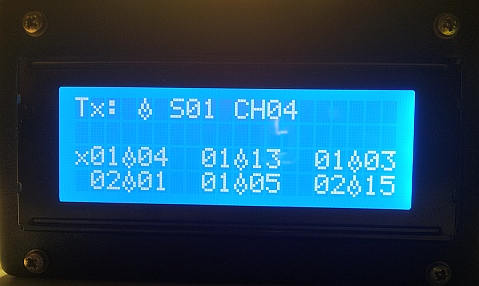
\includegraphics[width=.7\textwidth]{Bilder/SenderAnzeige}
					\caption{LCD während der Show}
					\label{fig:senderanzeige}
				\end{figure}

				In den Zeilen 3 und 4 werden die letzten sechs gesendeten Kommandos aufgelistet. Zwei zweistellige Zahlen getrennt durch ein Flammensymbol stehen dabei für einen Zündbefehl. Die erste Zahl gibt die Slave-ID, die zweite den zu zündenden Kanal an. Für den Fall, dass eine Aufforderung zur Identifikation gesendet wurde, erscheint \enquote{IDENT}, für eine Aufforderung zur Temperaturmessung \enquote{TEMP}. Das \enquote{x} steht immer vor dem bis dato letzten Befehl, springt also mit jedem neuen Befehl eine Stelle weiter.

				Alle Zeilen werden nach einer bestimmten Zeit automatisch gelöscht.

			\section{Schalter an den Zündboxen}

				Die Zündboxen verfügen, wie in Abbildung~\ref{fig:schalterzuend} zu erkennen, über zwei Schalter, einen schwarzen Wippschalter zum Ein- und Ausschalten der Energieversorgung sowie einen Schlüsselschalter, um die Zündbox \enquote{scharf} zu schalten.

				\begin{figure}[!b]
					\centering
					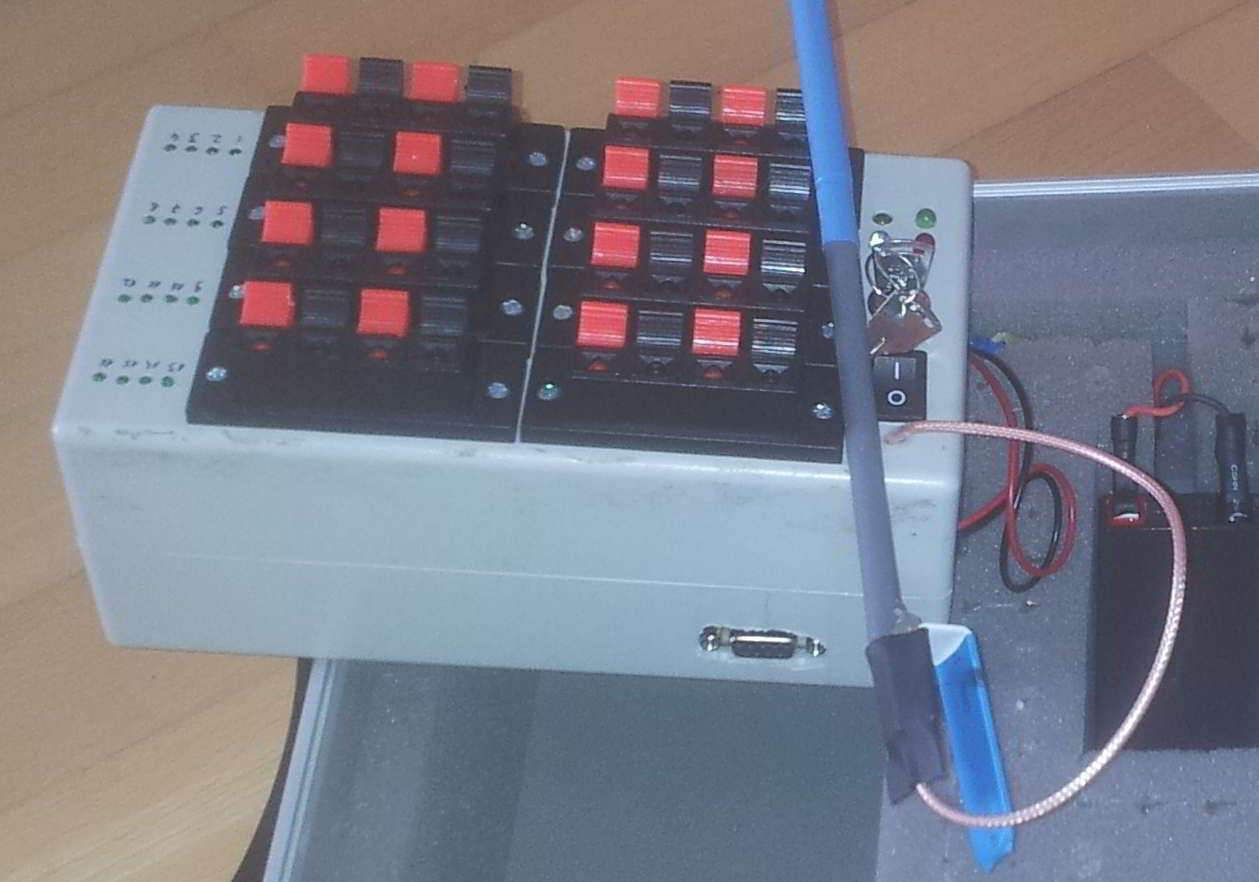
\includegraphics[width=.6\textwidth]{Bilder/SchalterZuendbox}
					\caption{Schalter und serielle Schnittstelle an der Zündbox}
					\label{fig:schalterzuend}
				\end{figure}

				Die Scharfschaltung durch den Schlüsselschalter geschieht auf die Weise, dass durch eine Zustandsabfrage vor der Zündung letztere nur ausgeführt wird, wenn das Schloss auf den grünen Punkt am Gehäuse zeigt. Befindet sich der Schlüssel in waagrechter Stellung und zeigt auf den roten Punkt, so ist der Schalter geöffnet und Zündbefehle werden von der Box ignoriert. Für das Scharfschalten der Box ist der Anwender selbst verantwortlich.

				Ob Boxen scharf geschaltet sind, ist an der Box~-- wie in Abschnitt~\ref{ch:leds} ausgeführt~-- durch das Dauerleuchten der roten Status-LED erkennbar, kann aber auch durch eine Identifizierungsabfrage ausgelesen werden (siehe Abschnitt~\ref{sec:config}).

		\chapter{Vorbereitung des PCs}

			Zur Kommunikation mit einem Computer verfügen alle Devices über eine serielle Schnittstelle. {\pic} sollte ohnehin auf dem Rechner installiert sein, für die serielle Kommunikation gibt es für Windows zudem zahlreiche Terminalprogramme.

			\section{Installation eines USB-RS232-Adapters}
				\label{sec:usbadapter}

				Zunächst steht man allerdings in der Regel vor dem Problem, dass zwar die Devices eine serielle Schnittstelle besitzen, moderne Rechner aber nicht mehr mit dem früher standardmäßig verbauten 9-poligen Sub-D-Stecker der RS232-Schnittstelle ausgestattet sind. Diese wurden seit dem Ende der 1990er-Jahre von den USB-Schnittstellen verdrängt. Sollte wider Erwarten am einzusetzenden Rechner ein derartiger Anschluss vorhanden sein, können die nächsten Absätze übersprungen und der COM-Port direkt im Gerätemanager anhand von Tabelle~\ref{tab:seriell} konfiguriert werden. Wer nur über USB-Ports verfügt, lese unmittelbar weiter.

				Weil in vielen Bereichen noch immer auf RS232 zurückgegriffen wird, existieren Adapterkabel wie in Abbildung~\ref{fig:transmitter} mit USB-Anschluss für den Rechner und einem 9-poligen RS232-Stecker für den Anschluss an der Peripherie, also die Devices von {\anlage}. In diesen Adapterkabeln ist ein Chip verbaut, um die Signalumsetzung von USB auf RS232 und umgekehrt zu bewerkstelligen. Übliche verwendete Chips sind der CH340\footnote{Treiber CH340/341: \url{http://wch.cn/download/list.asp?id=5}}, welcher sich in vielen über eBay aus China angebotenen Modellen befindet, der Prolific PL2303\footnote{Falls die automatische Treiberinstallation unter Windows fehlschlägt, funktioniert~-- mit zeitweiligen Aussetzern~-- oft der Treiber unter: \url{http://www.cartft.com/support/drivers/TFT/tftdrivers/GPS/PL2303_Prolific_GPS_1013_20090319.zip}} in verschiedenen Versionen oder~-- bei edleren und somit auch teureren Varianten~-- der uneingeschränkt zu empfehlende FTDI232, mit welchem die in den folgenden Abschnitten beschriebenen Probleme nicht auftreten sollten.

				Das Plug-and-Play-Traum\-szenario, dass sich der Adapter bei der Verbindung des USB-Steckers mit dem Rechner automatisch korrekt installiert, tritt gerade bei den günstigen Adaptern leider nur sehr selten ein. Die in den Fußnoten verlinkten Treiber sollten, sofern die automatische Treiberinstallation von Windows versagt, ihren Dienst tun, müssen allerdings teilweise mit sanfter Gewalt installiert werden. Hat man die Installation erfolgreich absolviert, sollte bei angeschlossenem Adapterkabel ein neuer Eintrag in der Art von Abbildung~\ref{fig:geraetemanager} im Gerätemanager auftauchen.

				Weil viele Chips dazu tendieren, sich beim Anschluss an immer wieder andere USB-Ports neu zu installieren bzw. eine andere COM-Port-Nummer anzunehmen, wird empfohlen, für den USB-RS232-Adapter stets denselben USB-Steckplatz zu nutzen.

				\begin{figure}
					\centering
					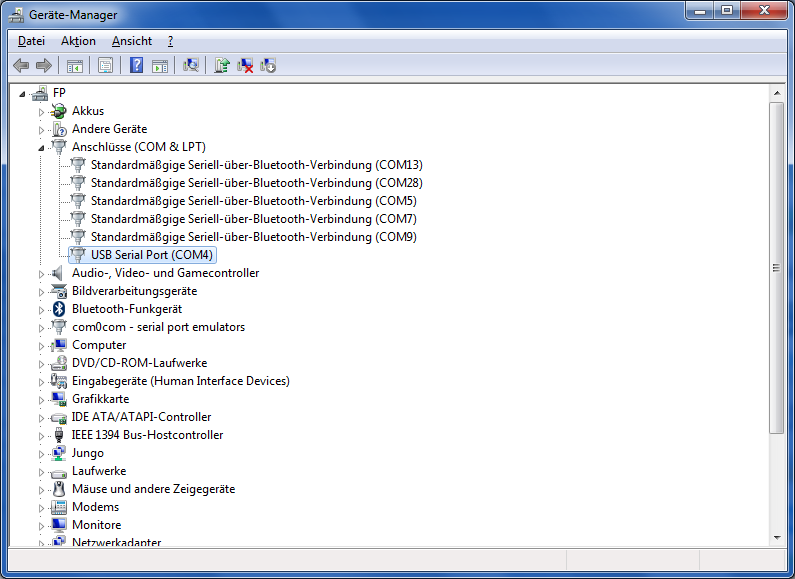
\includegraphics[width=.9\textwidth]{Bilder/geraetemanager}
					\caption{Eintrag des USB-RS232-Adapters im Gerätemanager}
					\label{fig:geraetemanager}
				\end{figure}

				Durch Doppelklick auf den Eintrag und den Reiter Anschlusseinstellungen kann die nun vorhandene serielle Schnittstelle unter Windows konfiguriert werden. Um Kompatibilität mit {\pic} zu gewährleisten, ist das Hauptfenster nach Tabelle~\ref{tab:seriell} zu konfigurieren.

				\begin{table}[b]
					\begin{center}
						\begin{tabularx}{7cm}{Xl}
							\hline\hline
							Bits pro Sekunde & 9600     \\
							Datenbits        & 8        \\
							Parität          & keine    \\
							Stoppbits        & 1        \\
							Flusssteuerung   & Hardware \\ \hline\hline
						\end{tabularx}
						\caption{Konfiguration der seriellen Schnittstelle}
						\label{tab:seriell}
					\end{center}
				\end{table}

				Unter der Schaltfläche \enquote{Erweitert} kann man zudem die Puffer ausschalten, was aber nicht zwingend notwendig ist und die Funktionsweise normalerweise weder positiv noch negativ beeinflusst, sowie die Portnummer für den neu geschaffenen COM-Port einstellen.

			\section{Einrichtung des Terminalprogramms}

				Hardware- und treiberseitig steht einer erfolgreichen Kommunikation von Rechner und Devices nun nichts mehr im Wege, für eine komfortable Unterhaltung außerhalb von {\pic} fehlt aber noch die entsprechende Software. Empfohlen wird die Verwendung des kostenlosen Programms \emph{Puttytel}\footnote{Herunterzuladen unter: \url{http://www.chiark.greenend.org.uk/~sgtatham/putty/download.html}}, mit welchem auch die im Rahmen dieser Anleitung gezeigten Beispiele durchgeführt werden. Es besteht nur aus einer einzigen ausführbaren Datei.

				\begin{figure}
					\centering
					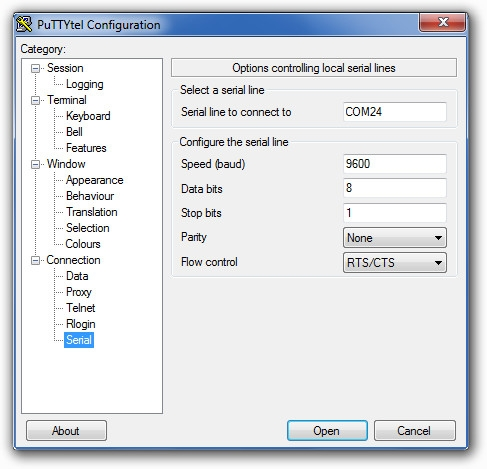
\includegraphics[width=.75\textwidth]{Bilder/puttytelstart}
					\caption{Einstellungen für \texttt{Puttytel}}
					\label{fig:puttytelstart}
				\end{figure}

				\texttt{Puttytel} kann per Doppelklick gestartet werden, woraufhin man zu einem Startbildschirm, der Kategorie \enquote{Session} gelangt. Man wählt in der linken Spalte unten links \enquote{Serial} und stellt die Parameter~-- analog zur Konfiguration des COM-Ports nach Tabelle~\ref{tab:seriell}~-- wie in Abbildung~\ref{fig:puttytelstart} ein. Anschließend muss man in der linken Spalte zurück auf \enquote{Session} gehen und dort im rechten Teil des Fensters \enquote{Serial} als \enquote{Connection Type} wählen, ehe man die serielle Verbindung per Klick auf \enquote{Open} starten kann. Vor dem Start der Verbindung sollte man zudem das verbundene Device mit Strom versorgen, damit dieses seine Kommunikationsschnittstelle vor Beginn des Datenaustauschs initialisieren kann.

				Um bei \texttt{Puttytel} nicht immer alle Einstellungen per Hand vornehmen zu müssen, bietet sich an, unter Windows eine Verknüpfung auf \texttt{puttytel.exe} zu erstellen und in den Ver\-knüpfungs\-eigen\-schaften als Ziel anzugeben:
				\begin{center}
					\verb|"c:\programme\puttytel\puttytel.exe" -serial com24 -sercfg 9600,8,1,n,R|
				\end{center}

				Die ohne Leerzeichen auf \enquote{com} folgende Zahl ist natürlich entsprechend dem verwendeten seriellen Anschluss (COM5, COM37, \dots) anzupassen.

			\section{Einrichtung von \pic}
				\label{sec:piceinrichtung}

				Um eine reibungslose Kommunikation zwischen {\pic} und {\anlage} sicherzustellen, muss in {\pic} als wesentliche Einstellung unter dem Menüpunkt \enquote{Einstellungen $\rightarrow$ Optionen} im Reiter \enquote{Output}~-- gezeigt in Abbildung~\ref{fig:pic-comport}~-- der richtige COM-Port eingestellt werden. Über \enquote{Einstellungen $\rightarrow$ Connect} wird die serielle Verbindung aufgebaut und in der untersten Leiste anzeigt, ob der Verbindungsaufbau erfolgreich war.

				Zudem sollte im Reiter \enquote{Allgemein} die globale Verzögerung erfahrungsgemäß, wie Abbildung~\ref{fig:pic-delay} zeigt, auf etwa 0,07\,s eingestellt werden. Dies ist die Zeit, die aufgrund von Datenübertragungen und Rechenvorgängen zwischen dem Beginn des Sendens des Befehls vom PC zum Transmitter und dem Zünden des Kanals an der Zündbox vergeht.

				Als minimale Zeitdauer zwischen zwei Zündungen sollte \SI{100}{\milli\second} nicht unterschritten werden, das Scharfschalten vor Beginn der Show ist ebenso nicht zu vergessen wie das Scharfschalten des Transmitters und sämtlicher Zündboxen!

				\textbf{Anmerkung: Eine serielle Verbindung zu einem Device kann immer nur durch einen einzigen Client (\texttt{Putty\-tel}, \texttt{GUI}, \texttt{\pic}, \texttt{Firware-Updater}) bestehen. Man muss also immer die bestehende Verbindung trennen, bevor man mit einem anderen Programm eine neue aufbauen kann.}

				\begin{figure}
					\begin{subfigure}[t]{\textwidth}
						\centering
						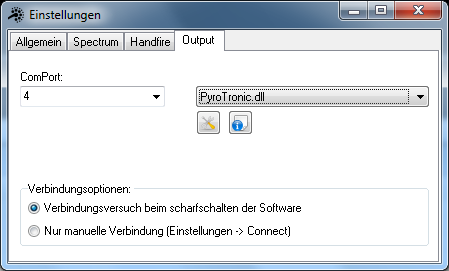
\includegraphics[width=.75\textwidth]{Bilder/pic-comport}
						\caption{Einstellung des COM-Ports in {\pic}}
						\label{fig:pic-comport}
					\end{subfigure}
					\\[50pt]
					\begin{subfigure}[t]{\textwidth}
						\centering
						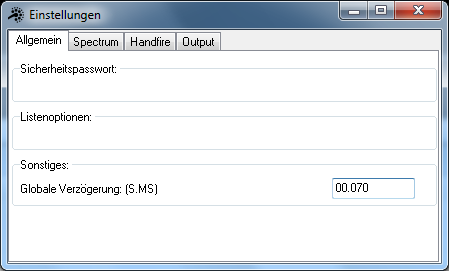
\includegraphics[width=.75\textwidth]{Bilder/pic-delay}
						\caption{Einstellung des Global Delay in \pic}
						\label{fig:pic-delay}
					\end{subfigure}
					\caption{Einstellungen in {\pic}}
				\end{figure}

		\chapter{Kommunikation zwischen PC und Devices}
			\label{ch:kommunikationpc}

			In diesem Abschnitt wird die Systemüberwachung bzw. -konfiguration über die serielle Schnittstelle mittels \texttt{Puttytel} oder die {\anlage}-GUI behandelt.

			Auf die Kommunikation zwischen {\pic} und der Transmitterbox wird an dieser Stelle nicht detailliert eingegangen, da hier~-- wenn alle Einstellungen wie in Abschnitt~\ref{sec:piceinrichtung} erläutert getroffen wurden~-- alles quasi-automatisch und ohne Zutun des Benutzers stattfindet. Es muss dafür aber unbedingt sichergestellt sein, dass das von {\pic} angesprochene Device scharfgeschaltet sein muss. Dies geschieht bei Zündboxen via Schlüsselschalter, bei Transmittern über den Terminalbefehl \enquote{arm}.

			Im Abschnitt \ref{ch:firmwareupdate} ab Seite \pageref{ch:firmwareupdate} wird das Aktualisieren der Firmware mittels Firmware-Updater erklärt.

			\section{Puttytel}

				\subsection{Befehlsübersicht}

					Hat man mittels \texttt{Puttytel} eine Verbindung zwischen einem Device und dem PC aufbauen können, sieht man vor sich zunächst nur einen schwarzen Bildschirm. Um nun mit dem Device kommunizieren zu können, existieren einige Befehle gemäß Tabelle~\ref{tab:commands}.

					\begin{table}[bt]
						\begin{center}
							\begin{tabularx}{.9\textwidth}{lX}
								\hline\hline
								\textbf{Befehl}                       & \textbf{Wirkung}                                                                                                                                                                                                                   \\ \hline
								arm                                   & Schaltet den Transmitter scharf, um Zündbefehle senden zu können                                                                                                                                                                   \\
								disarm                                & Schaltet den Transmitter unscharf, Zündbefehle werden nicht mehr gesendet                                                                                                                                                          \\ \hline
								\hyperref[subsec:localconf]{conf}     & Startet das Konfigurationsprogramm zur lokalen Zuweisung von Unique- und Slave-ID                                                                                                                                                  \\
								\hyperref[subsec:remoteconf]{remote}  & Startet das Konfigurationsprogramm zur ferngesteuerten Zuweisung von Unique- und Slave-ID                                                                                                                                          \\
								\hyperref[sec:list]{list}             & Zeigt die Systemübersicht (Zuweisung Unique- und Slave-ID, Batteriespannung jeder Box, Scharfschaltungsstatus Temperatur, RSSI, Anzahl Boxen je Slave-ID)                                                                          \\ \hline
								\hyperref[sec:manuellessenden]{send}  & Startet das Menü zur manuellen Eingabe einer Anweisung ans Funkmodul (Zündbefehl, Identifizierungsaufforderung oder Temperaturmessung)                                                                                             \\
								\hyperref[sec:manuellessenden]{fire}  & Führt zu einer Eingabemaske, in die Slave-ID und Kanal für die Zündung einzugeben sind                                                                                                                                             \\
								\hyperref[sec:manuellessenden]{ident} & Sendet eine Identifizierungsaufforderung an alle anderen Devices                                                                                                                                                                   \\
								\hyperref[sec:manuellessenden]{temp}  & Gibt über die serielle Schnittstelle die Temperatur aus und fordert alle anderen Devices ebenfalls zur Temperaturmessung auf. Zum Auslesen der neu gemessenen Temperaturen muss dann eine Identifizierungsanfrage geschickt werden \\ \hline
								\hyperref[sec:rfmzugriff]{rfm}        & Erlaubt unmittelbaren Zugriff auf das Funkmodul durch Eingabe einer 16-Bit-Hexadezimalzahl, um Registerwerte auszulesen oder neu zu setzen                                                                                         \\
								\hyperref[sec:encryption]{aeskey}     & Schlüssel für die Funkübertragung auslesen und neu setzen                                                                                                                                                                          \\ \hline
								orders                                & Gibt letztes gesendetes und empfangenes Pattern auf LCD aus                                                                                                                                                                        \\ \hline
								cls                                   & Löscht den Terminal-Bildschirm                                                                                                                                                                                                     \\
								kill                                  & Löst einen Neustart des Device aus                                                                                                                                                                                                 \\ \hline\hline
							\end{tabularx}
							\caption{Kommandos zur Konfiguration über die serielle Schnittstelle}
							\label{tab:commands}
						\end{center}
					\end{table}

					Diese können, sofern \texttt{Puttytel} die aktive Anwendung ist, direkt über die PC-Tastatur eingegeben werden und sollten zur unmittelbaren Ausführung mit Druck auf die Taste \emph{ENTER} abgeschlossen werden. Sobald das erste Zeichen eingegeben wurde, leuchtet die gelbe Status-LED am Device. Unbekannte Befehle werden ignoriert, sämtliche Buchstaben als Kleinbuchstaben interpretiert. Korrekturen sind unter Verwendung der \emph{BACKSPACE}-Taste möglich.

					Aufgrund der eingebauten Timeout-Funktion, welche ein Hängenbleiben des Programms während einer Show verhindern soll, bricht die Firmware die Eingabe ab, wenn zwischen der Eingabe der einzelnen Buchstaben mehr als $\SI{3}{\second}$ vergehen. Lässt man diese Zeit verstreichen, wird automatisch ein Drücken der \emph{ENTER}-Taste übermittelt, die Befehlseingabe also abgeschlossen und das Device ist unmittelbar bereit, einen neuen Befehl aufzunehmen. Wird also nach Eingabe eines gültigen Befehls die \emph{ENTER}-Taste nicht gedrückt, wird der Befehl durch den Timeout dennoch ausgelöst. Möchte man dies vermeiden, sollte man den Befehl vor Ausführung durch Eingabe weiterer Zeichen ungültig machen oder durch Entfernen aller Zeichen mittels \emph{BACKSPACE} löschen.

					Von den in Tabelle~\ref{tab:commands} aufgeführten Befehlen funktioniert lediglich \enquote{orders} nicht bei allen Devices, sondern setzt voraus, dass das angeschlossene Device ein Transmitter ist.

				\subsection{Konfiguration}
					\label{sec:config}

					\subsubsection{Lokal}
						\label{subsec:localconf}

						Mit \enquote{conf} gelangt man ins Konfigurationsmenü für die lokale Konfiguration der IDs, dessen Ablauf beispielhaft in Abbildung~\ref{fig:conf} gezeigt ist. Hier sind die beiden wichtigsten Parameter jeder Zündbox, die Unique-ID und die Slave-ID, aufgeführt, die der Benutzer nach eigenen Bedürfnissen vergeben kann.

						Die \textbf{Unique-ID} dient der Identifikation jeder einzelnen Zündbox im Funksystem. Jeder verwendeten Zündbox muss daher, um die Funktion von {\anlage} gewährleisten zu können, eine andere Unique-ID im Bereich von 01-30 (zweistellige Eingabe!) eineindeutig zugeteilt werden, d.\,h. jede Box hat eine unterschiedliche Unique-ID bzw. jede Unique-ID gehört zu genau einer Zündbox.

						Die \textbf{Slave-ID} entscheidet, auf welche Zündbefehle eine Zündbox reagiert. Sollen also zwei oder mehr Boxen stets zur selben Zeit denselben Kanal zünden, kann ihnen einfach die gleiche Slave-ID zugewiesen werden.

						Die Null als Unique- und Slave-ID identifiziert ein Device als Transmitterbox. Die Software erkennt dabei automatisch, ob es sich beim angeschlossenen Device grundsätzlich um einen Transmitter oder eine Zündbox handelt\footnote{Wie diese automatische Erkennung funktioniert, ist im Abschnitt \ref{ch:pinbelegung} ab Seite \pageref{ch:pinbelegung} beschrieben} und weist Transmittern unmittelbar beim Hochfahren \enquote{0} als Unique- und Slave-ID zu. Ein vom Aufbau her als Zündbox ausgeführtes Device muss immer von Null verschiedene IDs besitzen.

						Die Zuweisung von Unique- und Slave-ID vom Startbildschirm des Konfigurationsprogramms aus geschieht, indem man den Anweisungen auf dem Bildschirm folgt. Die Eingabe von \enquote{I} bzw. \enquote{i} (Groß- oder Kleinschreibung spielt keine Rolle) erlaubt eine Änderung von Unique- und Slave-ID einer Zündbox. Die neue Unique- bzw. Slave-ID muss stets zweistellig ohne Bestätigung durch \emph{ENTER} oder eine andere Taste eingegeben werden. Beide IDs können im Bereich von 01-30 liegen.

						\begin{figure}
							\centering
							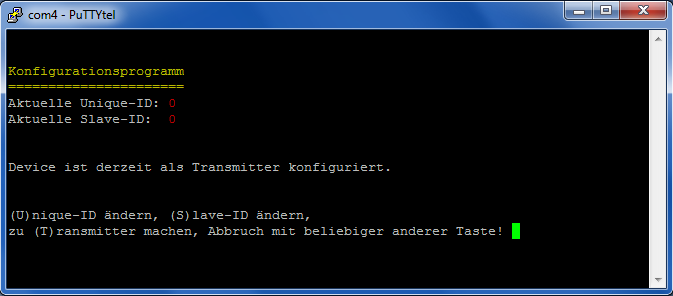
\includegraphics[width=.8\textwidth]{Bilder/conf}
							\caption{Ablauf des Konfigurationsprogramms bei Verbindung mit einer Zündbox}
							\label{fig:conf}
						\end{figure}

						Möchte man beispielsweise die Unique-ID 5 und die Slave-ID 12 zuweisen, muss man nach Anzeige des Startbildschirms zunächst \enquote{i} und anschließend \enquote{05} und \enquote{12} eingeben. Will man eine der beiden IDs beibehalten und nur die andere ändern, kann die Änderung durch Drücken von \emph{ENTER} übersprungen werden. Die zugewiesenen IDs werden an drei Stellen im internen Speicher mit Prüfsummen hinterlegt und bleiben sowohl nach dem Ausschalten als auch nach einem Firmwareupdate erhalten. Eine Änderung mindestens einer der IDs führt zu einem sofortigen Neustart der Zündbox.

						Unabhängig davon, dass eine Zündbox nicht als Transmitter konfiguriert werden, also nicht Unique- und Slave-ID  besitzen kann, kann sie theoretisch trotzdem zur Steuerung und Koordinierung eines Netzes und einer Show eingesetzt werden, indem man sie über die serielle Schnittstelle mit dem PC verbindet. Bis auf die Darstellung am LCD erfüllt sie dieselben Aufgaben wie ein Transmitter und kann auch parallel noch als Zündbox fungieren. Auf entsprechenden Sicherheitsabstand zu Lebewesen und sensibler Technik ist dabei selbstverständlich zu achten!

					\subsubsection{Ferngesteuert}
						\label{subsec:remoteconf}

						\begin{figure}
							\centering
							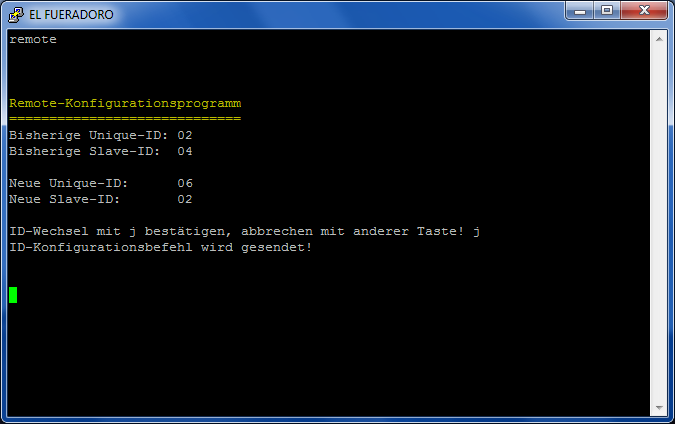
\includegraphics[width=.8\textwidth]{Bilder/remote}
							\caption{Beispiel einer ferngesteuerten ID-Zuweisung}
							\label{fig:remote}
						\end{figure}

						Über den Befehl \enquote{remote} gelangt man ins Konfigurationsprogramm zur ferngesteuerten Vergabe von Unique- und Slave-ID. Der Programmablauf ist beispielhaft in Abbildung~\ref{fig:remote} gezeigt: Die Eingabe der alten und neuen IDs erfolgt analog zur Eingabe bei lokaler Konfiguration, am Ende muss die Änderung noch bestätigt werden. Werden als alte Unique- und Slave-ID die Daten der verbundenen Box eingegeben, so werden deren Kennzahlen wie bei einer lokalen Konfiguration geändert und kein weiterer Befehl gesendet.

						Durch \enquote{remote} und die Eingabe von Unique- und Slave-ID einer nicht per Kabel verbundenen Box ist es möglich, die IDs einer eingeschalteten Zündbox per Funk zu ändern. Voraussetzung ist dabei, dass die angesprochene Zündbox nicht scharf geschaltet ist.

						Der Anwender hat selbst darauf zu achten, durch ein ferngesteuertes Update nicht einem Device eine bereits vergebene Unique-ID zuzuweisen! Falls dies dennoch geschieht, ist das weitere Vorgehen davon abhängig, ob die Devices auch die gleiche Slave-ID besitzen oder nicht. Sind die Slave-IDs nicht identisch, so kann durch einen weiteren \enquote{remote}-Befehl die Unique-ID-Zuweisung geändert werden. Bei identischen Slave-IDs funktioniert dies nicht, da stets alle Devices auf den Änderungsbefehl in gleicher Weise reagieren würden. Hier müssen daher alle Devices mit identischen IDs bis auf eines ausgeschaltet werden, dem man dann neue IDs zuweisen kann. Nun kann dann jeweils ein weiteres Device eingeschaltet und seine IDs neu gesetzt werden, bis wieder alle unterschiedliche Unique-IDs besitzen.

				\subsection{Systemübersicht}
					\label{sec:list}

					Mit \enquote{list} ist es möglich, sich die Systemübersicht entsprechend Abbildung~\ref{fig:list} anzeigen zu lassen. Es werden zwei Tabellen ausgegeben, wobei die obere nach Unique-ID geordnet anzeigt:
					\begin{enumerate}
						\item Slave-ID, welcher der Unique-ID zugewiesen ist.
						\item Spannung, welche die Batterie der Box mit der entsprechenden Unique-ID liefert.
						\item Scharfschaltungsstatus der Box mit der jeweiligen Unique-ID: (j)a (=scharf) oder (n)ein (=nicht scharf).
						\item Temperatur im Inneren der Box, sofern die Box über einen eingebauten Temperatursensor verfügt, ansonsten wird \enquote{n.a.}~(not available) angezeigt.
						\item Stärke des von der Box empfangenen Antwortsignals (RSSI = Received Signal Strength Indicator) in dBm. Je größer der Wert ist~-- bei negativen Werten also umso näher er bei 0 liegt, umso besser und umso weniger störanfällig ist die Verbindung zwischen den Devices. Die theoretische Empfangsgrenze liegt bei etwa $\SI{-96}{\dBm}$.
					\end{enumerate}

					Die untere Tabelle listet auf, wie viele Boxen mit der entsprechenden Slave-ID derzeit aktiv sind.

					Zwischen den beiden Tabellen wird die Anzahl der fehlerhaften IDs aufgelistet. Dies kann entweder auf doppelte Zuweisung von Unique-IDs oder Fehler beim Auslesen der IDs (fehlerhafte Prüfsummen) zurückzuführen sein. Für normalen Betrieb sollte dieser Wert stets 0 betragen.

					\begin{figure}
						\centering
						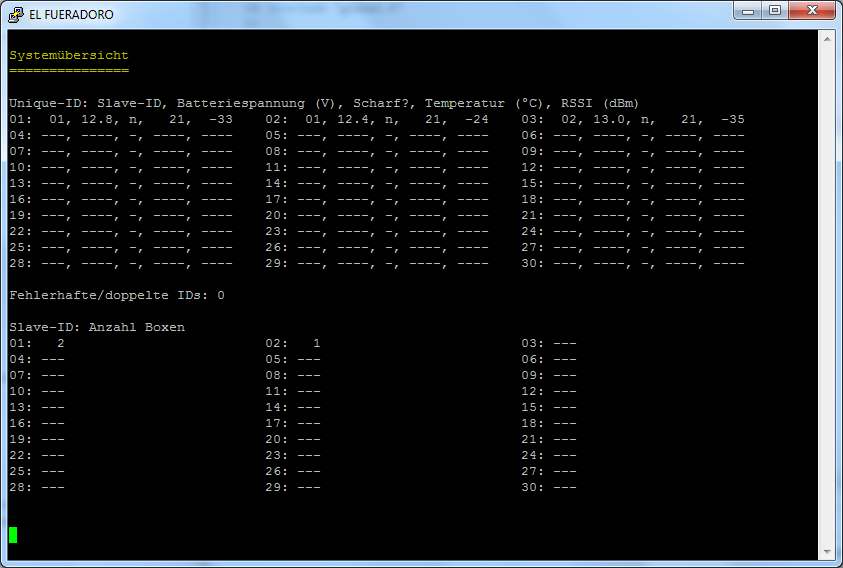
\includegraphics[width=.8\textwidth]{Bilder/list}
						\caption{Systemübersicht}
						\label{fig:list}
					\end{figure}

					Der dargestellte Zustand entspricht den empfangenen Parametern nach der letzten Identifikationsaufforderung bzw. nach dem Einschalten der Zündbox. Für eine möglichst aktuelle Liste sollte also vor dem Aufruf von \enquote{list}, wie im Abschnitt~\ref{sec:manuellessenden} beschrieben, eine Identifikationsaufforderung gesendet werden.

				\subsection{Manuelles Senden}
					\label{sec:manuellessenden}

					Zu Testzwecken oder um die Systemübersicht zu aktualisieren, können mittels \enquote{send} Zündbefehle und die Aufforderung zur Identifizierung oder Temperaturmessung manuell versendet werden. Nach Eingabe von \enquote{send} muss dies mit \enquote{f} (=fire), \enquote{i} (=identify) oder \enquote{t} (=temperature) ausgewählt werden. Wählt man \enquote{i} oder \enquote{t} ist keine weitere Eingabe nötig, bei \enquote{f} müssen anschließend noch Slave-ID und Kanal jeweils zweistellig eingegeben werden. Statt \enquote{send} und den entsprechenden Buchstaben anzugeben, können auch die direkten Befehle \mbox{\enquote{fire}}, \mbox{\enquote{ident}} und \mbox{\enquote{temp}} verwendet werden.

					Jede andere Angabe als \enquote{f}, \enquote{i} oder \enquote{t} beendet den Modus ohne irgendetwas zu senden. Denselben Effekt hat die Eingabe einer Slave-ID oder Kanalnummer außerhalb der jeweils zulässigen Zahlenbereiche.

				\subsection{Funkmodul-Zugriff}
					\label{sec:rfmzugriff}

					Die zwingend für den Betrieb von {\anlage} notwendigen Zugriffe auf das Funkmodul werden von der Software automatisch getätigt, so dass diese Funktion in der Regel nicht gebraucht wird. Dennoch ist es möglich das verwendete Funkmodul \texttt{RFM69CW\footnote{Link zum Datenblatt auf Seite~\pageref{sec:datasheets}}} unmittelbar über das Terminalprogramm anzusprechen, um Werte aus den Registern zu lesen oder die Register für die aktuelle Sitzung neu zu beschreiben. Beim nächsten Neustart des Devices werden stets die Standardeinstellungen wiederhergestellt, lediglich die Sendeleistung kann dauerhaft gespeichert werden.

					Nach Eingabe von \enquote{rfm} und Bestätigung mit \emph{ENTER} erscheint eine Aufforderung zur Befehls\-eingabe. Diese hat im Hexadezimalformat als 16-Bit-Wert zu erfolgen, d.\,h. vierstellig mit den zulässigen Zeichen 0-9 und A-F bzw. a-f. Jedes eingegebene Zeichen symbolisiert dabei vier Bits, die Umrechnung ist in Tabelle~\ref{tab:zahlensysteme} gezeigt.

					\begin{table}
						\begin{center}
							\begin{tabularx}{.8\textwidth}{X*{16}c}
								\hline\hline
								Hexadezimal & 0    & 1    & 2    & 3    & 4    & 5    & 6    & 7    \\
								Dezimal     & 0    & 1    & 2    & 3    & 4    & 5    & 6    & 7    \\
								Binär       & 0000 & 0001 & 0010 & 0011 & 0100 & 0101 & 0110 & 0111 \\
								\\
								Hexadezimal & 8    & 9    & A    & B    & C    & D    & E    & F    \\
								Dezimal     & 8    & 9    & 10   & 11   & 12   & 13   & 14   & 15   \\
								Binär       & 1000 & 1001 & 1010 & 1011 & 1100 & 1101 & 1110 & 1111 \\ \hline\hline
							\end{tabularx}
						\end{center}
						\caption{Umrechnung Hexadezimal-, Dezimal- und Binärwerte}
						\label{tab:zahlensysteme}
					\end{table}

					Die Bedeutung der Eingabe für das Funkmodul ist in Tabelle~\ref{tab:rfmcommand} illustriert. Hierbei sollte auch klar werden, wie sich die Werte für die Zeichen 1-4 zusammensetzen. Ist ein Bit gesetzt, muss die entsprechende Zahl (8, 4, 2, 1) zum Zeichenwert addiert werden, so dass sich bei vier gesetzten Bits als Maximalwert 15 ergibt, ist nur das oberste Bit gesetzt, lautet der Wert 8, ist nur das unterste gesetzt 1, sind die beiden mittleren Bits gesetzt 6, usw.

					Es ist zu erkennen, dass das erste einzugebende Zeichen sowohl das Schreiben/Lesen-Bit enthält als auch die obersten drei Bit der Registeradresse. Die acht Datenbits sind lediglich für einen Schreibbefehl relevant, bei einem Lesezugriff kann als drittes und viertes Zeichen ohne Konsequenzen ein beliebiger Hexadezimalwert im Bereich von 0x00 bis 0xFF übertragen werden.

					\begin{table}
						\begin{center}
							\begin{tabularx}{.95\textwidth}{Xc|*{7}c|*{8}c}
								\hline\hline
								Bit     & w/$\overline{\mbox{r}}$         & r6                              & r5                              & r4                            & r3 & r2 & r1 & r0                      & d7 & d6 & d5 & d4                      & d3 & d2 & d1 & d0                    \\
								Wert    & 8                               & 4                               & 2                               & \multicolumn{1}{c||}{1}       & 8  & 4  & 2  & \multicolumn{1}{c||}{1} & 8  & 4  & 2  & \multicolumn{1}{c||}{1} & 8  & 4  & 2  & \multicolumn{1}{c}{1} \\
								Zeichen & \multicolumn{4}{c||}{Zeichen 1} & \multicolumn{4}{c||}{Zeichen 2} & \multicolumn{4}{c||}{Zeichen 3} & \multicolumn{4}{c}{Zeichen 4}                                                                                                                          \\ ~ \\ \hline
							\end{tabularx}
							\begin{tabularx}{.95\textwidth}{p{2cm}cXp{2cm}}
								~                                                                                                      \\
								 & w/$\overline{\mbox{r}}$ & Schreib- oder Lesezugriff (0 = lesen, 1 = schreiben)                      \\
								 & r6 {\dots} r0           & Registeradresse                                                           \\
								 & d7 {\dots} d0           & Zu schreibender Registerwert (beliebig falls w/$\overline{\mbox{r}} = 0$) \\ \hline\hline
							\end{tabularx}
						\end{center}
						\caption{Struktur des \texttt{RFM69CW}-Befehls}
						\label{tab:rfmcommand}
					\end{table}

					\subsubsection{Auslesen der eingestellten Sendeleistung}
						\label{subsec:readpower}

						Zur Veranschaulichung soll hier die Abfrage der aktuell eingestellten Sendeleistung und eine anschließende Änderung derselben simuliert werden: Aus dem Datenblatt, dem die Bedeutungen aller Registeradressen und ihrer acht Registerbits zu entnehmen sind, kann die Registeradresse 0x11 als diejenige identifiziert werden, in der die Informationen zur Sendeleistung hinterlegt sind. Um nun den aktuellen Wert auszulesen, gibt man~-- wie in Abbildung~\ref{fig:rfmread} gezeigt~-- im Terminalprogramm \enquote{rfm} gefolgt von \emph{ENTER} ein und anschließend die Zeichenfolge \enquote{11FF}, wobei die beiden hinteren Stellen wie erwähnt keine Rolle spielen.

						\begin{figure}
							\centering
							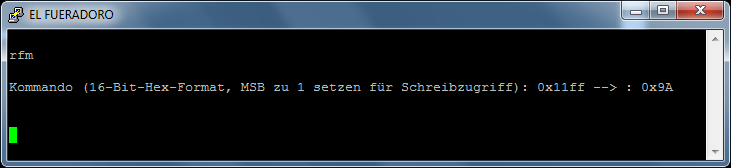
\includegraphics[width=.8\textwidth]{Bilder/rfmbefehl}
							\caption{Auslesen der gesetzten Sendeleistung}
							\label{fig:rfmread}
						\end{figure}

						Das Modul antwortet nun mit einem 8-Bit-Wert, z.\,B. mit dem Wert 0x9A, welcher dem Binärwert 10011010 entspricht, dessen Bedeutung dem Datenblatt entnommen werden kann: Das oberste Bit signalisiert, dass die Verstärkerstufe PA0 aktiv ist, die beiden folgenden Bits sind 0, da PA1 und PA2 in der Variante \texttt{RFM69CW} nicht genutzt werden können. Die unteren fünf Bits schließlich stehen für die eingestellte Sendeleistung, wobei man vom aus den fünf Bits berechneten Wert noch 18 abziehen muss, um die Sendeleistung in dBm zu erhalten. Gesetzt sind die Bits 4, 3 und 1, was dem Wert 26 ($= 2^4 + 2^3 + 2^1$) entspricht, daraus resultiert eine eingestellte Sendeleistung von $\SI{8}{\dBm}$.

					\subsubsection{Setzen der Sendeleistung}

						Will man die Sendeleistung nun auf $\SI{6}{\dBm}$ anpassen, muss also ein Wert von 24 für die Aus\-gangs\-lei\-stungs-Bits gesetzt werden, dazu natürlich auch das oberste Bit für den PA0. Als Wert für die Registerbits ergibt sich damit $2^7 + 2^4 + 2^3 = 0x98$. Die Registeradresse bleibt gleich, jedoch muss dem Modul mitgeteilt werden, dass es sich um einen Schreibzugriff handelt, weshalb die erste Stelle um den Wert 8 erhöht werden muss. Um nun den neuen Wert von $\SI{6}{\dBm}$ einzuschreiben, gibt man im Terminalprogramm~-- wie in Abbildung~\ref{fig:rfmwrite} gezeigt~-- \enquote{rfm} gefolgt von \emph{ENTER} ein und anschließend die Zeichenfolge \enquote{9198}.

						Als Antwort erhält man vom Modul den Registerwert von VOR dem Schreibzugriff, im Beispiel also den Wert 0x9A. Anschließend erfolgt eine Nachfrage, ob die Sendeleistung dauerhaft gespeichert werden soll. Verneint man dies, wird beim nächsten Neustart des Device der Standardwert wiederhergestellt, andernfalls ist der gerade eingestellte Wert der neue Standardwert.

						Ein nochmaliges Auslesen des Registers, wie im Abschnitt~\ref{subsec:readpower} beschrieben, sollte nun den eben eingeschriebenen Wert 0x98 zurückgeben.

						\begin{figure}
							\centering
							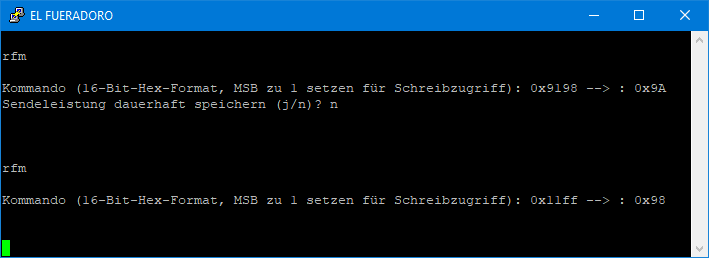
\includegraphics[width=.8\textwidth]{Bilder/rfmbefehl2}
							\caption{Setzen der Sendeleistung mit anschließendem Auslesen}
							\label{fig:rfmwrite}
						\end{figure}

				\subsection{AES-Verschlüsselung}
					\label{sec:encryption}

					Zum sicheren Betrieb von {\anlage} werden die drahtlos zu übermittelnden Daten zwischen Sender und Empfänger verschlüsselt. Hierfür muss in den am Funkverkehr beteiligten Modulen ein Schlüssel mit einer Länge von 16~Bytes (128~Bit) hinterlegt werden, der für die Ver- und Entschlüsselung der Datenpakete genutzt wird. Dieser Schlüssel ist im internen Speicher des Mikrocontrollers hinterlegt und bleibt auch beim Trennen der Stromversorgung erhalten. Selbstredend muss in allen Controllern derselbe Schlüssel hinterlegt sein, damit diese miteinander kommunizieren können.

					Nach Eingabe von \enquote{aeskey} im Terminalfenster kann der aktuell eingestellte Schlüssel eingesehen werden. Hierzu wird der Schlüssel einmal aus dem Speicher des Controllers ausgelesen und einmal aus den Einstellungen des Funkmoduls. Diese beiden Zeilen sollten identische Werte anzeigen.
					
					Jede Taste außer \enquote{s} bringt den Benutzer anschließend ins Hauptmenü zurück.

					Möchte man den Schlüssel ändern, muss die Taste \enquote{s} gedrückt und anschließend der komplette neue Schlüssel im hexadezimalen Zahlenformat eingegeben werden, wie beim Funkmodul-Zugriff sind also nur die Zeichen 0-9 und A-F bzw. a-f zulässig. Wurde ein gültiger Schlüssel eingegeben, erfolgt noch eine finale Nachfrage, ob dieser neue Schlüssel gespeichert werden soll, welche man mit \enquote{j} oder \enquote{n} beantworten kann.
					\clearpage

			\section{GUI}

				\begin{figure}[!h]%
					\centering
					\begin{subfigure}[t]{0.45\textwidth}
						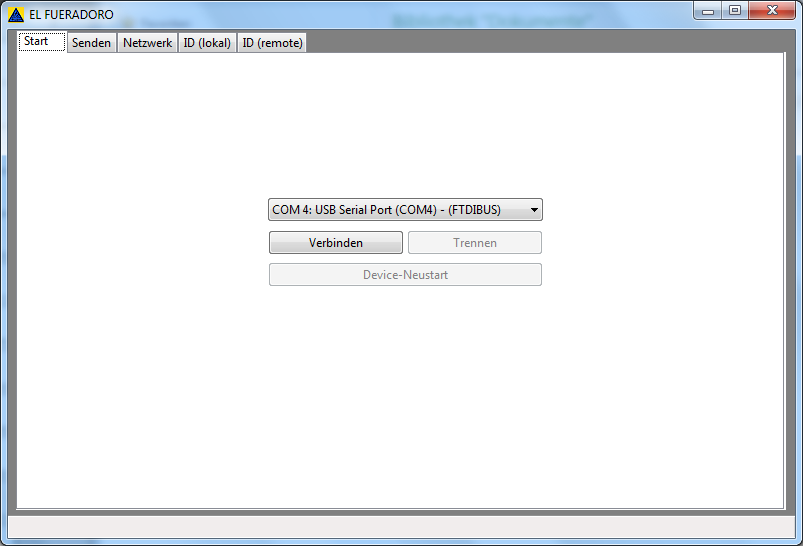
\includegraphics[width=\textwidth]{bilder/gui-start}
						\caption{Keine serielle Verbindung}
						\label{fig:gui-unconnected}
					\end{subfigure}
					%
					\begin{subfigure}[t]{0.45\textwidth}
						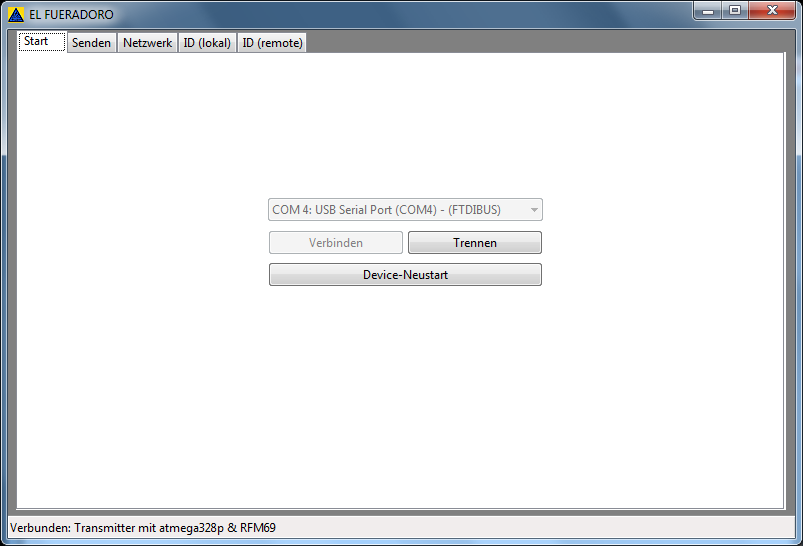
\includegraphics[width=\textwidth]{bilder/gui-connected}
						\caption{Verbindung erfolgreich hergestellt}
						\label{fig:gui-connected}
					\end{subfigure}
					%
					\caption{Startbildschirm der GUI}
					\label{fig:gui-start}
				\end{figure}
				%

				Die GUI stellt eine graphische Oberfläche zur Implementierung der \texttt{Puttytel}-Funktionen dar, indem über die serielle Schnittstelle ein- und ausgehende Daten geparst und an den entsprechenden Stellen innerhalb der Oberfläche dargestellt werden. Die Software ist in die fünf Reiter \enquote{Start}, \enquote{Senden}, \enquote{Netzwerk}, \enquote{ID~(lokal)} und \enquote{ID~(remote)} unterteilt, in denen die entsprechenden Funktionen ausgeführt werden können.

				Nach dem Start der Software sind alle Schaltflächen in allen Reitern mit Ausnahme der Auswahl der zur Verfügung stehenden COM-Ports und der Schaltfläche \enquote{Verbinden} im Reiter \enquote{Start} ausgegraut und deaktiviert, was in Abbildung~\ref{fig:gui-unconnected} dargestellt ist. Nach Auswahl des entsprechenden Ports und Klick auf \enquote{Verbinden}, werden diese beiden Schaltflächen ausgegraut und deaktiviert. Im Gegenzug erscheint in der Fußleiste der Devicetyp mit verwendetem Controller und Funkmodul und die Schaltflächen \enquote{Trennen} sowie \enquote{Device-Neustart} werden im aktuellen Reiter aktiv (Abbildung~\ref{fig:gui-connected}).%
				%
				\begin{figure}[!b]
					\centering
					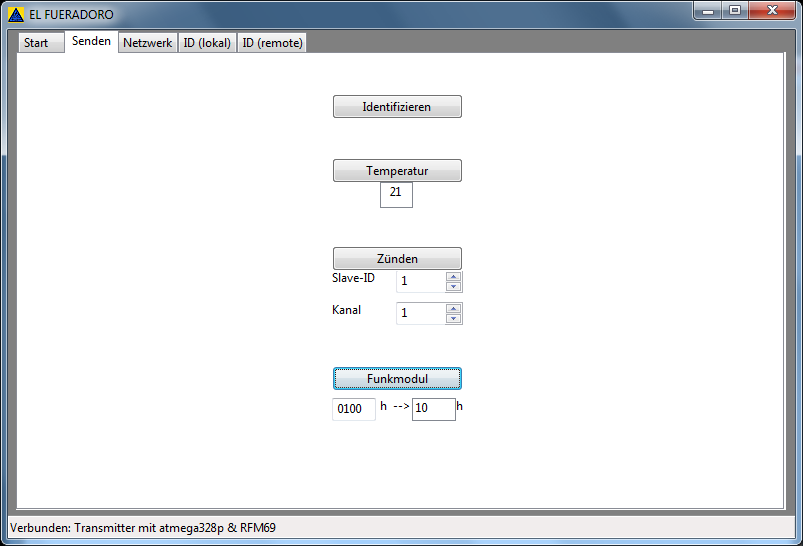
\includegraphics[width=0.5\textwidth]{bilder/gui-senden}
					\caption{Sendebildschirm der GUI}
					\label{fig:gui-senden}
				\end{figure}

				Nach Herstellung der Verbindung sind auch die sonstigen Schaltflächen aktiv, Abbildung~\ref{fig:gui-senden} zeigt den Reiter \enquote{Senden} im aktiven Zustand. Hier kann per Klick eine Identifizierungsaufforderung verschickt, eine Temperaturmessung getriggert, ein Zündvorgang ausgelöst oder ein Befehl ans Funkmodul geschickt werden. Bei \enquote{Zünden} und \enquote{Funkmodul} ist darauf zu achten, dass beim Klick auf die Schaltfläche unmittelbar die aktuell in den Eingabefeldern stehenden Werte übertragen werden, man diese also vor dem Klicken anpassen muss. Bei Temperaturanfrage und Funkmodulzugriff wird im entsprechenden Anzeigefeld die Antwort des angeschlossenen Devices~-- also die Temperatur in Grad Celsius oder die Antwort des Funkmoduls auf den aktuellen Registerzugriff als 8-bit-Hexadezimalwert~-- ausgegeben. Das permanente Ändern der Sendeleistung ist in der GUI noch nicht implementiert.

				Der Reiter \enquote{Netzwerk} (Abbildung~\ref{fig:gui-netzwerk}) dient einzig und allein der Darstellung der aktuell im System befindlichen Zündboxen mit ihren Parametern Unique-ID, Slave-ID, Batteriespannung, Scharf\-schaltungs-Status, Temperatur und gemessenem RSSI-Wert beim Empfang der Parameter.

				\begin{figure}[!t]
					\centering
					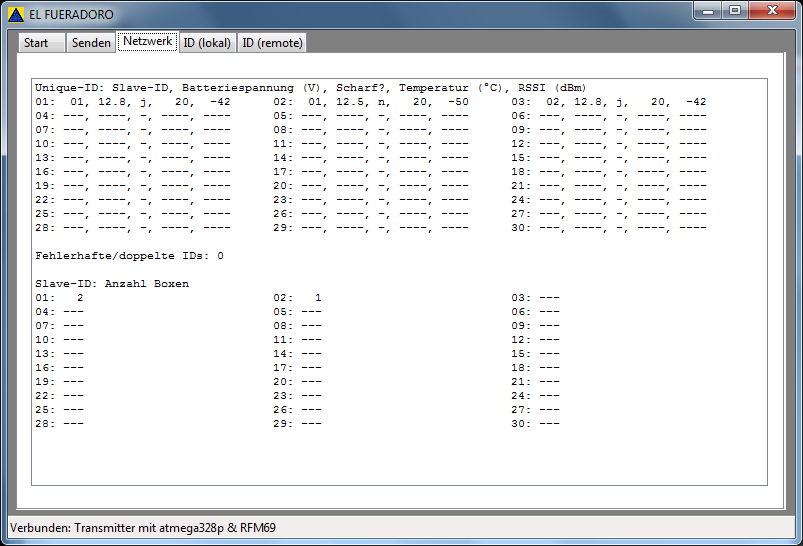
\includegraphics[width=0.5\textwidth]{bilder/gui-netzwerk}
					\caption{Netzwerkanzeige der GUI}
					\label{fig:gui-netzwerk}
				\end{figure}

				Die Ansicht des Reiters \enquote{ID~(lokal)} ist, wie Abbildung~\ref{fig:gui-local} zeigt, abhängig vom angeschlossenen Devicetyp. Bei Transmittern sind die Schaltflächen deaktiviert, da hier keine Änderungen an den IDs vorgenommen werden können (Abbildung~\ref{fig:gui-local-trans}). Bei Zündboxen werden bei Aufruf des Reiters die aktuellen IDs in die entsprechenden Felder kopiert, können verändert und die Änderungen dann durch Klick auf \enquote{Werte übernehmen} übernommen werden (Abbildung~\ref{fig:gui-local-ig}).

				\begin{figure}[!b]
					\centering
					\begin{subfigure}[t]{0.45\textwidth}
						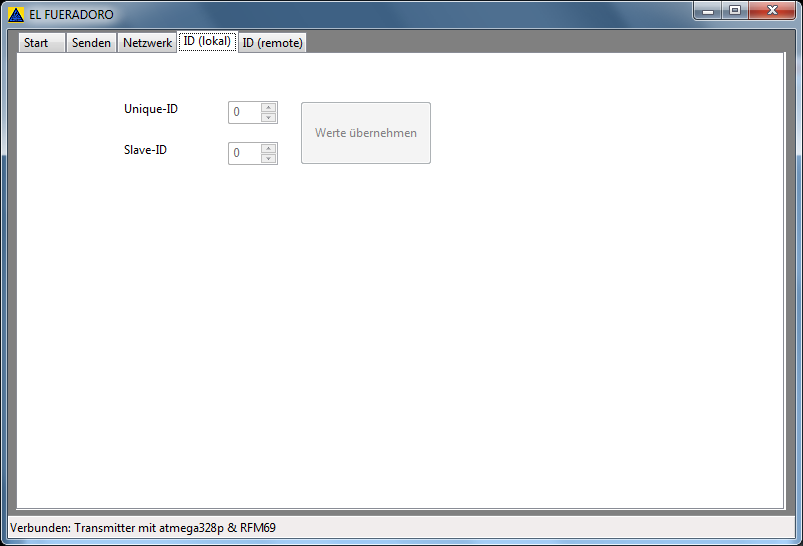
\includegraphics[width=\textwidth]{bilder/gui-local-trans}
						\caption{Transmitter}
						\label{fig:gui-local-trans}
					\end{subfigure}
					%
					\begin{subfigure}[t]{0.45\textwidth}
						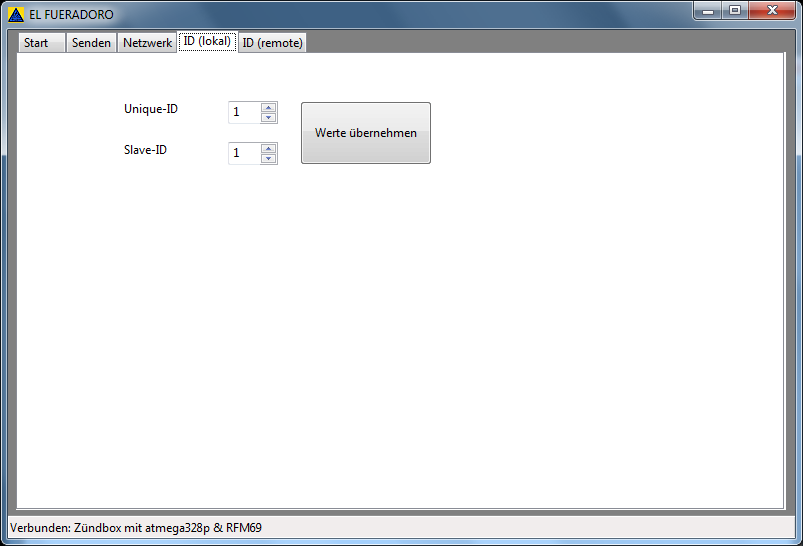
\includegraphics[width=\textwidth]{bilder/gui-local-ig}
						\caption{Zündbox}
						\label{fig:gui-local-ig}
					\end{subfigure}
					\caption{Lokale ID-Konfiguration}
					\label{fig:gui-local}
				\end{figure}

				Im Reiter \enquote{ID~(remote)} können alte und neue ID-Kombination eingestellt werden. Durch Klick auf \enquote{Ausführen} wird der Befehl zur ID-Änderung gesendet.

				\begin{figure}[!t]
					\centering
					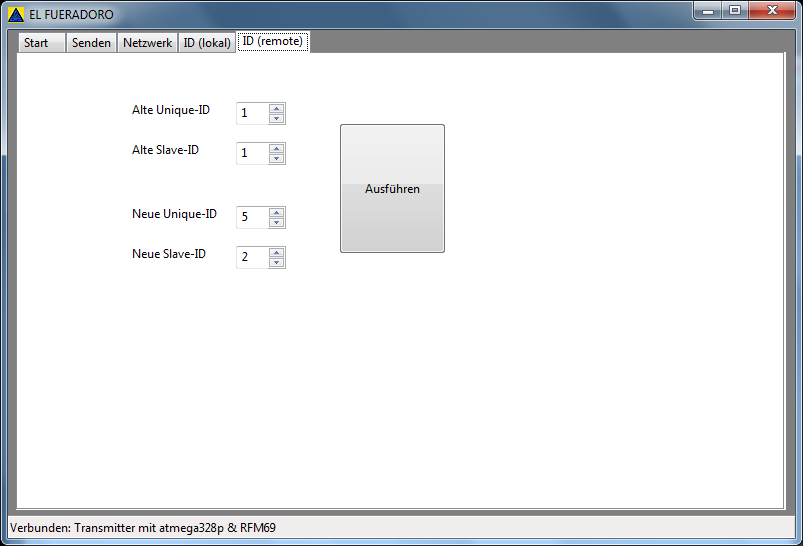
\includegraphics[width=0.45\textwidth]{bilder/gui-remote}
					\caption{Remote-ID-Einstellung}
					\label{fig:gui-remote}
				\end{figure}

		\chapter{Der Raspberry-Pi-Transmitter}

			Als Alternative zur Kombination aus Laptop/PC und dem in den vorangegangenen Abschnitten beschriebenen Transmitter wurde in Zusammenarbeit mit einem Softwareentwickler ein Audio-Funksystem auf Basis des bekannten Einplatinencomputers Raspberry Pi entwickelt. Dieser übernimmt die Kontrolle der Show inklusive der Musikwiedergabe.

			Neben einem Raspberry Pi werden für den Aufbau eine speziell für die Verwendung mit {\anlage} entwickelte Aufsteckplatine sowie ein Touchdisplay, eine USB-Soundkarte, zwei Taster, ein Schlüsselschalter und zwei LEDs benötigt. Eine Einkaufsliste findet sich in Tabelle~\ref{tab:raspibom} ab Seite \pageref{tab:raspibom}.

			Die Spannungsversorgung kann man entweder über den Micro-USB-Anschluss am Raspberry Pi oder über U\textsubscript{Force} an der linken Stiftleiste herstellen. Wird einer dieser beiden Anschlüsse mit einer Spannungsquelle verbunden, muss der jeweils andere offen bleiben!

		\chapter{Show}

			\section{Vorbereitung}

				\subsection{Beidseitiges Zünden}
					Gerade in Musikfeuerwerken steht man häufig vor der Herausforderung, ein durch die Dramaturgie des Musikstücks sehr genau abgestecktes Zeitintervall mit Effekten füllen zu müssen. Ist die Laufzeit einer Cakebox länger als dieses Intervall und besitzt der Effekt eine Reservezündschnur, kann die Laufzeit durch eine weitere Zündung an der Reservezündschnur entsprechend verkürzt werden.

					Ab dem Zeitpunkt der zweiten Zündung wird die Restlaufzeit der Batterie halbiert, da die Anzündlitze dann von beiden Seiten abbrennt. Bezeichnet man das Zeitintervall zwischen erster und zweiter Zündung mit ${\Delta}t$ und die ursprüngliche Laufzeit als $T_\text{original}$, ergibt sich die neue Laufzeit $T_\text{neu}$, die zwischen der halben und der ganzen ursprünglichen Laufzeit liegen kann, aus
					\begin{equation}
						T_\text{neu} = \frac{T_\text{original} + {\Delta}t}{2}.
						\label{eq:gegenzuendung}
					\end{equation}

					Durch Umstellen der Formel \eqref{eq:gegenzuendung} kann der Abstand zwischen den beiden Zündzeitpunkten bei festgelegter neuer Laufzeit bestimmt werden:
					\begin{equation}
						{\Delta}t = 2 {\cdot} T_\text{neu} - T_\text{original}
					\end{equation}

					Soll also eine Batterie mit einer Laufzeit von $\SI{60}{\second}$ in $\SI{40}{\second}$ abgebrannt werden, muss die zweite Zündung $\SI{20}{\second}$ nach der ersten ausgelöst werden. Hierbei kommt es natürlich auch zu einer Verdichtung der Effekte.

				\subsection{Zündkreisauslegung}

					An dieser Stelle soll kurz auf die Grenzen und Limits von {\anlage} eingegangen werden, die bei der Planung einer Show zu berücksichtigen sind. Die Charakteristika und Kennwerte der einzelnen Anzündertypen sind Anlage 2 der 1.\,SprengV zu entnehmen.

					{\anlage} ist für die Verwendung mit den Anzündertypen A (Auslösestrom $\SI{0,6}{\ampere}$) und U (Auslösestrom $\SI{1,3}{\ampere}$) ausgelegt. Der nötige Strom zum Auslösen eines HU-Anzünders (Auslösestrom $\SI{25}{\ampere}$) kann nicht geliefert werden. Es ist zu berücksichtigen, dass in der Anlage ein Strombegrenzungswiderstand von $\SI{2,2}{\ohm}$ verbaut ist, der in Reihe zum angeschlossenen Anzünder-Netzwerk liegt. Mittels Formel~\eqref{eq:zuendkreisrmax} kann der maximal zulässige Widerstand (inklusive der $\SI{2,2}{\ohm}$) für einen gegebenen mittleren Strom $I$ ermittelt werden.

					\begin{equation}
						R_\text{max} = \frac{50}{47 {\cdot} \ln\left(\frac{\SI{423}{\ampere}}{\SI{423}{\ampere} - 20 {\cdot} I}\right)}\si{\ohm}
						\label{eq:zuendkreisrmax}
					\end{equation}

					Entsprechend resultiert für einen gegebenen Widerstand der mittlere Strom über eine Zeit von $\SI{10}{\milli\second}$ aus Gleichung~\eqref{eq:zuendkreisi}.

					\begin{equation}
						I = \SI{21,15}{\ampere} {\cdot} \left(1 - \mathrm{e}^{-\frac{\SI{50}{\ohm}}{47 {\cdot} R}}\right)
						\label{eq:zuendkreisi}
					\end{equation}

					Einige Kennwerte für Ströme und die resultierenden maximalen Widerstände sind in Tabelle~\ref{tab:r-vs-i} aufgeführt.

					\begin{table}
						\centering
						\begin{tabular}{SSS}
							\hline\hline
							{Strom (A)} & {Widerstand gesamt ($\Omega$)} & {Widerstand Anzünder + Kabel ($\Omega$)} \\ \hline
							0,6         & 37,0                           & 34,8                                     \\
							0,75        & 29,5                           & 27,3                                     \\
							0,9         & 24,5                           & 22,3                                     \\
							1,0         & 22,0                           & 19,8                                     \\
							1,2         & 18,2                           & 16,0                                     \\
							1,5         & 14,5                           & 12,3                                     \\
							1,75        & 12,3                           & 10,1                                     \\
							2           & 10,7                           & 8,5                                      \\
							2,5         & 8,5                            & 6,3                                      \\ \hline\hline
						\end{tabular}
						\caption{Widerstandswerte für Zündkreise bei gegebenem Strom}
						\label{tab:r-vs-i}
					\end{table}

					Der Kabelwiderstand kann unter Kenntnis von Querschnittsfläche $A$ und/oder Durchmesser $d$, Material (mit spezifischem Widerstand $\rho$) und Kabellänge $l$ berechnet werden:

					\begin{equation*}
						\begin{split}
							R_\text{Kabel} & = \frac{\rho {\cdot} l}{A}                                  \\
							& \text{bzw.}                                                 \\
							R_\text{Kabel} & = \frac{4 {\cdot} \rho {\cdot} l}{d^2  {\cdot} {\symup\pi}}
						\end{split}
					\end{equation*}

					Für einige typische Drahtmaterialien ist der spezifische Widerstand in Tabelle~\ref{tab:spezwiderstand} dargestellt. Je kleiner der spezifische Widerstand ausfällt, umso größer ist dementsprechend sein Kehrwert, die elektrische Leitfähigkeit.

					\begin{table}
						\centering
						\begin{tabular}{lS}
							\hline \hline
							Material  & {$\rho \left(\si{\ohm\square\milli\metre\per\metre}\right)$} \\ \hline
							Silber    & 0,0159                                                       \\
							Kupfer    & 0,0175                                                       \\
							Aluminium & 0,0265                                                       \\
							Eisen     & 0,15                                                         \\
							Stahl     & 0,2                                                          \\ \hline\hline
						\end{tabular}
						\caption{Spezifischer Widerstand verschiedener Leitermaterialien}
						\label{tab:spezwiderstand}
					\end{table}

					Bei der Verwendung von Verschleißdraht mit einer Kupferseele mit Durchmesser $d = \SI{0,5}{\milli\metre}$ kann für Überschlagsrechnungen also davon ausgegangen werden, dass je $\SI{10}{\metre}$ Kabel-Gesamtweg (also Hin- und Rückleitung addiert) ein zusätzlicher Reihenwiderstand von $\SI{1}{\ohm}$ im Zündkreis auftritt.

					Setzt man pro A-Anzünder einen Widerstand von $\SI{2}{\ohm}$ und pro U-Anzünder einen Widerstand von $\SI{0,8}{\ohm}$ an und geht von einem Gesamt-Kabelweg von $\SI{10}{\metre}$ aus, sollte die Anlage also im Stande sein, eine Reihe von 10\,A-Anzündern, wodurch sich $R_\text{ges} = \SI{23,2}{\ohm}$ ergibt, noch sicher auszulösen, da der mittlere Strom dann noch mehr als $\SI{50}{\%}$ über dem Auslösestrom eines A-Anzünders liegt. Bei den U-Anzündern ergibt sich unter sonst gleichen Bedingungen, was Stromüberhöhung und Kabellänge angeht, ebenso eine Maximalzahl von 10\,U-Anzündern in Reihe.

					\textbf{Es sei noch einmal deutlich darauf hingewiesen, dass aufgrund der unterschiedlichen Widerstände und Ansprechströme niemals verschiedene Anzündertypen zusammen in einem Zündkreis verwendet werden sollten~-- und zwar weder in Reihen- noch in Parallelschaltung!}

					Eine Beispielrechnung macht dies klar: Würde man beispielsweise je fünf Anzünder jeder Kategorie zu einer Reihenschaltung von 10 Anzündern zusammenschalten, ergäbe sich $R_\text{ges} = \SI{17,2}{\ohm}$ und damit nach Formel \eqref{eq:zuendkreisi} ein Strom $I = \SI{1,27}{\ampere}$, was bereits unterhalb des spezifizierten Auslösestroms eines U-Anzünders ($\SI{1,3}{\ampere}$) liegt.

					Hinzu kommt bei gleichen Anzündern die Problematik, dass selbst bei einem rechnerisch ausreichend hohen Strom, dieser wahrscheinlich nicht über die notwendige Zeitspanne bei den U-Anzündern ankäme. Dies liegt am unterschiedlichen Zündimpuls (Einheit \si{\milli\watt\second\per\ohm}), hinter dem sich der bei Schmelzsicherungen als Schmelzintegral bekannte \enquote{I-Quadrat-t-Wert}, also das Produkt aus dem Quadrat des Stroms und der Zeit, verbirgt\footnote{$\si{\watt} = \si{\volt\ampere}$ und $\si{\ohm} = \si{\volt\per\ampere}$ $\Rightarrow$ $\si{\watt\per\ohm} = \si{\square\ampere}$}. Fließt derselbe Strom durch die Reihenschaltung eines Anzünders vom Typ A und einen Anzünder vom Typ U, löst der A-Anzünder aufgrund des geringeren notwendigen Zündimpulses zuerst aus. Durch das Auslösen wird in aller Regel der Stromkreis unmittelbar unterbrochen, so dass kein Strom mehr durch den U-Anzünder fließen kann, weshalb die ihn ihm umgesetzte Energie nicht zum Auslösen ausreicht.

					Die Krux bei einer Parallelschaltung, welche gegenüber der Reihenschaltung ohnehin die schlechtere Alternative darstellt, verschiedener Anzündertypen liegt darin, dass ein Auslösen des Anzünders nicht zwingend gleichbedeutend mit einer Unterbrechung des Stromkreises ist. Bei einer Parallelschaltung unterschiedlicher Widerstände wird zunächst der Ast mit dem geringsten Widerstand auslösen, allerdings kann nicht garantiert werden, dass dieser anschließend auch wirklich einen elektrischen Leerlauf darstellt. Sehr häufig ist auch nach dem Ansprechen noch eine elektrisch leitende Verbindung zwischen den Anzünderdrähten messbar, so dass ein Auslösen der weiteren Äste~-- gerade im Fall stark unterschiedlicher Widerstände~-- nicht gesichert ist.

					{\anlage} ermöglicht das Auslösen in so kurzen Zeitabständen, dass derartige Drahtseilakte durch eine Aufteilung auf zwei kurz hintereinander erfolgende Zündungen vermieden werden können.

					\textbf{Dem Anwender wird empfohlen, bei gleichzeitigem Zünden mehrerer Anzünder gleichen Typs eine Reihenschaltung zu verwenden}, da hierdurch die Fehleranfälligkeit und Ausfallwahrscheinlichkeit deutlich verringert wird.

					Ein Leerlauf (kein Durchgang eines Anzünders oder schlechte Kabelverbindung) wird bei der Reihenschaltung unmittelbar durch die nicht-leuchtende Kanal-LED bemerkt, bei einem Kurzschluss eines Anzünders fällt lediglich der Effekt dieses einen Anzünders aus. Bei der Parallelschaltung sorgt der Kurzschluss eines Anzünders mit hoher Wahrscheinlichkeit dafür, dass alle parallel geschalteten Anzünder stromlos bleiben, auch wird ein Leerlauf aufgrund des über die anderen Anzünder geschlossenen Stromkreises vermutlich nicht bemerkt.

				\subsection{Funkreichweite}

					Die Frage nach der Funkreichweite, also wie weit die Zündboxen bei {\anlage} vom Transmitter entfernt sein dürfen, um noch sicher auszulösen, kann pauschal nicht beantwortet werden, da dieser Wert sehr vielen Einflussgrößen unterliegt.

					Das theoretische Reichweiten-Maximum bei der verwendeten Frequenz von \SI{868}{\mega\hertz} und einer zulässigen Dämpfung von \SI{113}{\decibel} (Sendeleistung in dBm minus niedrigste Empfangsleistung in dBm) ergibt sich aus der Friis-Übertragungsgleichung zu mehreren Kilometern. Hierfür müssten die Antennen jedoch mehrere Meter über dem Erdboden angebracht sein, um ideale Wellenausbreitung durch die Luft und Entkopplung vom Boden zu ermöglichen, was in der Feuerwerks-Praxis meist nicht umsetzbar ist, und die Umgebung müsste so störungsfrei sein, dass der Empfänger das Signal auch bei sehr geringen Leistungen noch detektieren kann.

					In Tests mit {\anlage} konnte für ein reales Szenario (Platzierung im Gras am Boden) eine Distanz von \SI{250}{\meter} zwischen Sender und Empfänger mit einer Reserve von über \SI{20}{\decibel} gegenüber der minimalen Empfänger\-empfindlichkeit überbrückt werden, was für die meisten Feuerwerke ausreichend sein dürfte. Wichtig ist hierbei jedoch eine Sichtverbindung zwischen den Devices. Bricht diese Sichtlinie ab, sinkt die Reichweite, da eine Verbindung über reflektierende und streuende Hindernisse in aller Regel stark verlustbehaftet ist.

					Für eine möglichst hohe Reichweite sollte man die Devices daher mit möglichst ungestörter Sichtlinie zueinander und so weit wie möglich vom Boden entfernt platzieren. Die Antennen sollten möglichst parallel zueinander ausgerichtet sein.

					In der Systemübersicht, die in Abbildung~\ref{fig:list} auf Seite~\pageref{fig:list} zu sehen ist, wird dargestellt, wie stark die anderen Devices vom angeschlossenen Device empfangen werden.

				\subsection{Erstellung und Überprüfung des Zündplans}

					{\pic} unterstützt den Ersteller einer Show, indem es sowohl den passenden Zündzeitpunkt aus den Angaben \enquote{Effektbeginn} und \enquote{Verzögerung} berechnet als auch anhand der angegebenen Effektdauer die Überlagerung der Effekte kalkuliert und veranschaulicht.
					\pic{} wird den eingegebenen Zündplan perfekt umsetzen, die Krux liegt jedoch darin, dass falsche Eingaben des Erstellers übernommen und nicht hinterfragt werden.

					Wenig ist ärgerlicher, als dass eine sorgfältig geplante Show an Flüchtigkeitsfehlern scheitert. Ein falscher Klick bei der Erstellung des Zündplans kann dafür sorgen, dass die Highlightbatterie nicht angesprochen wird und statt buntem Lichterzauber nur schwarze Nacht am Himmel zu sehen ist. Aus diesem Grund existiert das auf {\anlage} zugeschnittene Tool \texttt{schemecheck.exe}, welches folgende Dinge im Zündplan erkennen kann und hinweist auf:
					\begin{itemize}
						\item Verwenden einer Slave-ID außerhalb des Bereichs $1-30$
						\item Ansprechen eines Kanals außerhalb des Bereichs $1-16$
						\item Unterschreiten des minimalen Zündabstands von $\SI{100}{\milli\second}$
						\item Mehrfachzünden derselben Slave-Kanal-Kombination
					\end{itemize}
					Darüber hinaus werden auch alle angesprochenen Slave-IDs und die Gesamtzahl der Cues angezeigt.

					Zur Überprüfung muss der in {\pic} erstellte Zündplan als zpl-Datei gespeichert und dem Kommandozeilentool folgendermaßen übergeben werden:
					\begin{center}
						\emph{schemecheck.exe fw.zpl}
					\end{center}

			\section{Durchführung}

				Die Durchführung eines Feuerwerks mit allen bürokratischen, logistischen, sicherheitstechnischen und sonstigen Herausforderungen ist Gegenstand eigener Lehrbücher und Vorschriften, weshalb hier nur auf den Einsatz von {\anlage} eingegangen werden soll.

				Hierbei gilt ebenso wie in vielen anderen Lebensbereichen der Spruch \enquote{Ordnung ist das halbe Leben}. Die Anzünderkabel sollten beschriftet und derart verlegt werden, dass man bei einer eventuellen Fehlersuche schnell fündig wird, zudem sollte ihre Länge so kurz wie möglich aber so lang wie nötig dimensioniert werden, um keine zu hohen Leitungswiderstände zu produzieren, aber auch keine Stolperfallen.

				Vor Aufbau der Zündkoffer gilt es, für jede Zündbox eine geeignete Position mit genügendem Abstand zu den Effekten zu finden, um ein Übergreifen entstehender Brände auf den Koffer und die Zündbox zu verhindern. An diesen Positionen werden die Enden der Anzünderkabel für jede einzelne Box gesammelt.

				Nun kann der jeweilige Koffer platziert und geöffnet werden, im ersten Schritt wird die Antenne angebracht und fest an der Buchse an der Zündbox verschraubt, ehe man die metallischen Teile der Schraubverbindung mit einem Klebestreifen gegen Berührungen mit freiliegenden Kabeln isoliert. Anschließend kann der Akku verbunden werden. Um böse Überraschungen zu vermeiden, sollte man die Box einschalten und mit dem Transmitter kontrollieren, ob sie an dieser Position erreichbar ist.

				Im nächsten Schritt muss, falls noch nicht geschehen, der Schlüsselschalter auf Position \enquote{rot} gedreht und abgezogen werden. Erst dann dürfen die Anzünderkabel angeschlossen werden, zunächst an der schwarzen, dann an der zugehörigen roten Klemme. Sind alle Kabel angeklemmt, kann man die Box einschalten, dabei durch das Blinken der gelben und organgen Status-LEDs sicherstellen, dass sie auf die korrekte Slave-ID programmiert ist, und anhand der Kanal-LEDs überprüfen, ob auf allen angeschlossenen Kanälen ein geschlossener Stromkreis vorliegt. Ist letzteres nicht der Fall, müssen zunächst Kabelverbindungsstellen kontrolliert werden. Erweisen die sich als in Ordnung und sind auch die einzelnen Kabelwege niederohmig, so dass ein Kabelbruch ausgeschlossen werden kann, müssen die Anzünder kontrolliert und eventuell getauscht werden. Zum Schutz der Zündbox vor Wetter und sonstigem Niederschlag ist der Kofferdeckel nach Abschluss der Arbeiten zu schließen, vorher kann die Box zur Batterieschonung erst einmal wieder abgeschaltet werden. Ein Abdecken der Boxen mit Brandschutzmatten kann in Erwägung gezogen werden, die Antenne sollte zwecks Empfang aber immer frei sein und senkrecht nach oben zeigen.

				Das Scharfschalten der Boxen darf als allerletzter Schritt erst unmittelbar vor dem Beginn der Show erfolgen. Mit einem Identifikationsbefehl vom Transmitter und anschließender Betrachtung der Empfängerliste kann kontrolliert werden, ob alle Boxen erreichbar und scharf geschaltet sind. Fällt auf, dass eine Box die falsche Slave-ID besitzt, muss sie zunächst wieder entschärft werden, bevor man einen Remote-ID-Wechsel durchführen kann.

				Sind diese Arbeiten erledigt und der Transmitter scharf geschaltet, kann das Terminalprogramm/die GUI beendet werden und {\pic} gestartet werden. Hier den Zündplan öffnen, verbinden und scharfschalten~-- jetzt kann der Spaß endlich losgehen!

		\chapter{Firmwareupdate}
			\label{ch:firmwareupdate}

			\textbf{WICHTIG: Aus Sicherheitsgründen darf kein Update durchgeführt werden, solange Anzünder mit dem Device verbunden sind, da sich die Devices im Falle eines Übertragungsfehlers völlig unvorhersehbar verhalten können.}

			\section{Herunterladen}

				Die aktuelle Firmware kann aus dem Git-Repository
				\begin{center}
					\url{https://github.com/fixxl/el-fueradoro}
				\end{center}
				mittels Git-Client oder direkt über den Link
				\begin{center}
					\url{https://github.com/fixxl/el-fueradoro/archive/master.zip}
				\end{center}
				heruntergeladen werden.

				Im Repository enthalten sind der komplette C-Quellcode, das AVR-Eclipse-Projekt, die kom\-pilierten iHex-Dateien für Firmware und Bootloader, die nötigen Software-Tools zur Übertragung zwischen PC und Mikrocontroller sowie die vorliegende Anleitung.

			\section{Aktualisierung}

					{\anlage} bietet die Möglichkeit, die Firmware via serielle Schnittstelle vom PC aus zu aktualisieren. Hierfür stehen das Kommandozeilentool \emph{fwupdate.exe} oder eine Windows-Oberfläche namens \texttt{UpdateLoader}, welche beide zunächst einenReset auslösen, um den Bootloader des Devices zu aktivieren, und anschließend die im iHex-Format vorliegende Firmware überträgen.

				Es existieren zwei grundsätzlich identische Firmwareversionen, welche sich nur in der standardmäßig eingestellten Sendeleistung des Funkmoduls unterscheiden. In der Standardversion ist eine geringere Sendeleistung eingestellt, in der \enquote{High Power}-Firmware, ist die Sendeleistung des Funkmoduls standardmäßig auf den Maximalwert gesetzt, so dass sich zwei verschiedene Firmwaredateien gemäß Tabelle~\ref{tab:firmwareversions} im gleichen Ordner wie \emph{fwupdate.exe} und \emph{UpdateLoader.exe} befinden.

				\begin{table}
					\centering
					\begin{tabularx}{.925\textwidth}{Xccc}
						\hline\hline
						Firmware                        & Controller  & Funkmodul & Sendeleistung   \\ \hline
						Pyro\_atmega328p\_RFM69.hex     & ATMEGA 328P & RFM69CW   & $\SI{8}{\dBm}$  \\
						Pyro\_atmega328p\_RFM69\_HP.hex & ATMEGA 328P & RFM69CW   & $\SI{13}{\dBm}$ \\ \hline\hline
					\end{tabularx}
					\caption{Verfügbare Firmware-Versionen}
					\label{tab:firmwareversions}
				\end{table}

				\subsection{Kommandozeile}

					\emph{fwupdate.exe} muss über die Kommandozeile mit zwei Parametern gestartet werden, nämlich der Angabe der seriellen Schnittstelle und dem Namen der zu übertragenden Firmware-Datei. Um nun die neue Firmware zu übertragen, lautet das Kommando für ein Device am \emph{COM4} mit dem \emph{ATmega328P} (und dem Funkmodul \emph{RFM69CW}):

					\begin{center}
						\emph{fwupdate.exe /c4 /fm:Pyro\_atmega328p\_RFM69.hex}
					\end{center}

					oder für die Firmware mit höherer Sendeleistung

					\begin{center}
						\emph{fwupdate.exe /c4 /fm:Pyro\_atmega328p\_RFM69\_HP.hex}
					\end{center}

					Die Angabe der Dateiendung \emph{.hex} kann hierbei~-- ebenso wie das \emph{.exe} hinter \emph{fwupdate}~-- auch weggelassen werden, die Firmware-Datei muss jedoch zwingend auf \emph{.hex} enden.

					\emph{fwupdate.exe} ist, sofern bereits eine korrekt funktionierende Firmware auf dem Device vorhanden ist, in der Lage, automatisiert zu ermitteln, welche Firmwaredatei die benötigte ist, das Kommando für ein Update über \emph{COM4} lautet dann nur noch:

					\begin{center}
						\emph{fwupdate.exe /c4 /fa}
					\end{center}

					Der Updater führt nach Übertragung der Daten einen CRC-Check durch. Sollte dieser fehlschlagen, wurde die Firmware nicht korrekt übertragen. Dies kann zufällig passieren oder auf ein Hardwareproblem, welches in der Regel beim USB-RS232-Adapter liegt, zurückzuführen sein. Für den Fall eines CRC-Fehlers sollte die Firmware erneut übertragen werden. Bleibt das Update beim Punkt \enquote{COMx at 9600 baud:} stehen, sollte die Stromversorgung des Device kurz unterbrochen und wieder aktiviert werden. Das Kabel für die serielle Verbindung bleibt währenddessen mit Device und PC verbunden.

				\subsection{Windows-Oberfläche}

					Dank der Arbeit von Leo-Andres Hofmann\footnote{Seine Homepage findet sich unter: \url{https://luani.de}} existiert die in Abbildung~\ref{fig:updateloader} dargestellte Windows-Oberfläche zur einfachen Übertragung der Firmware via serielle Schnittstelle, der \texttt{UpdateLoader}. Hier kann man aus der Liste der verfügbaren COM-Ports den entsprechenden wählen sowie die zu übertragende Datei einstellen und die Dateiübertragung per Klick auf \enquote{Update starten} durchführen.

					\begin{figure}[!h]
						\centering
						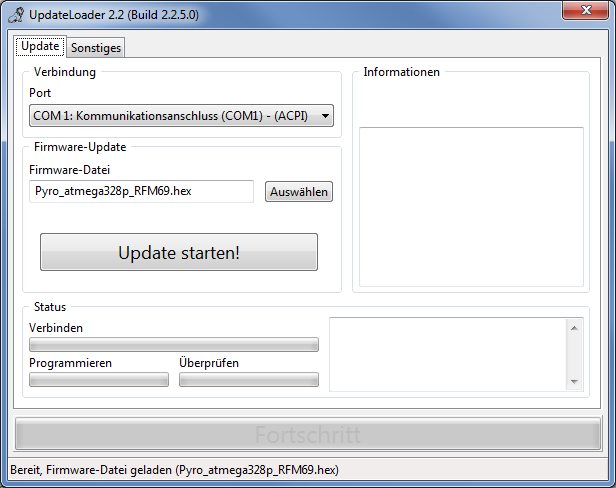
\includegraphics[width = .66\textwidth]{Bilder/updateloader.png}
						\caption{Benutzeroberfläche \texttt{UpdateLoader}}
						\label{fig:updateloader}
					\end{figure}

	\part{Dokumentation}
		\label{part:dokumentation}

		\chapter{Schaltpläne \& Layouts}

			In den Abbildungen~\ref{fig:transmitterschematic} und~\ref{fig:zuendboxschematic} sind die Schaltpläne von Transmitter und Zündbox nach Funk\-tions\-ein\-heiten unterteilt gezeigt, in den Abbildungen~\ref{fig:transmitterlayout} und~\ref{fig:zuendboxlayout} die Layouts. Erstellt wurden diese mit der Layoutsoftware \texttt{EAGLE} von CadSoft, die Originaldateien sind im Unterordner \enquote{Schematics\_and\_Layouts} des Projekt-Hauptverzeichnisses abgelegt.

			Die Layouts der ersten Generation wurden dabei so gestaltet, dass die Platinen nicht zwingend zweiseitig gefertigt werden müssen. Die Anzahl der Leiterbahnen auf der Oberseite wurde minimiert, zudem verlaufen sie nicht unterhalb von Bauelementen und können daher als Drahtbrücken ausgeführt werden. Die zweite Generation der Zündboxplatine wurde hingegen als typische Zwei-Lagen-Platine entworfen.

			Die Abmessungen der Platinen finden sich in Abschnitt~\ref{ch:platinenherstellung} auf Seite~\pageref{ch:platinenherstellung}.

			\begin{figure}
				\centering
				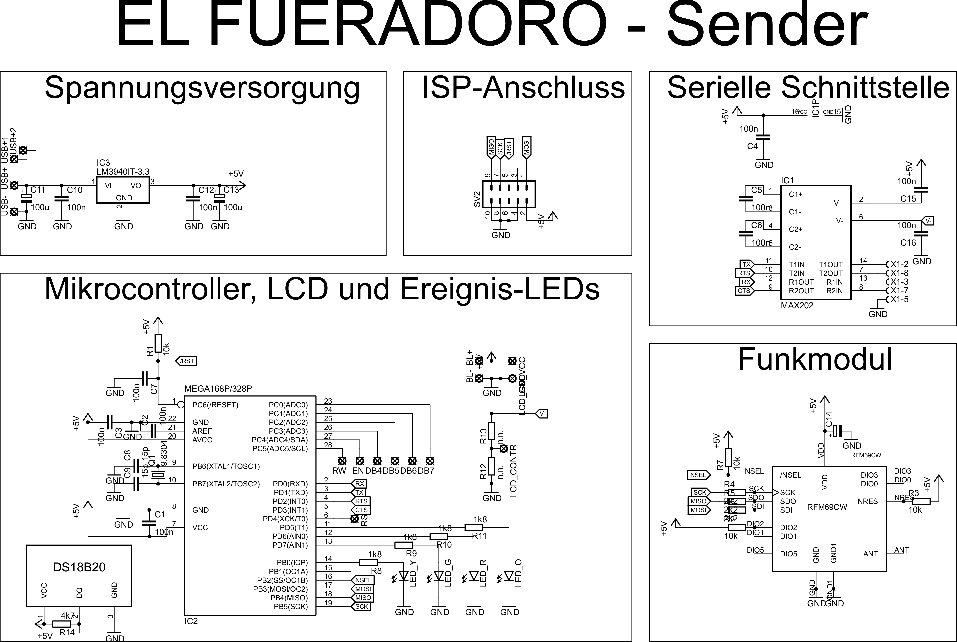
\includegraphics[angle=-90, width=.9\textwidth, keepaspectratio]{Bilder/Transmitterschaltplan}
				\caption{Schaltplan des Transmitters}
				\label{fig:transmitterschematic}
			\end{figure}

			\begin{figure}
				\centering
				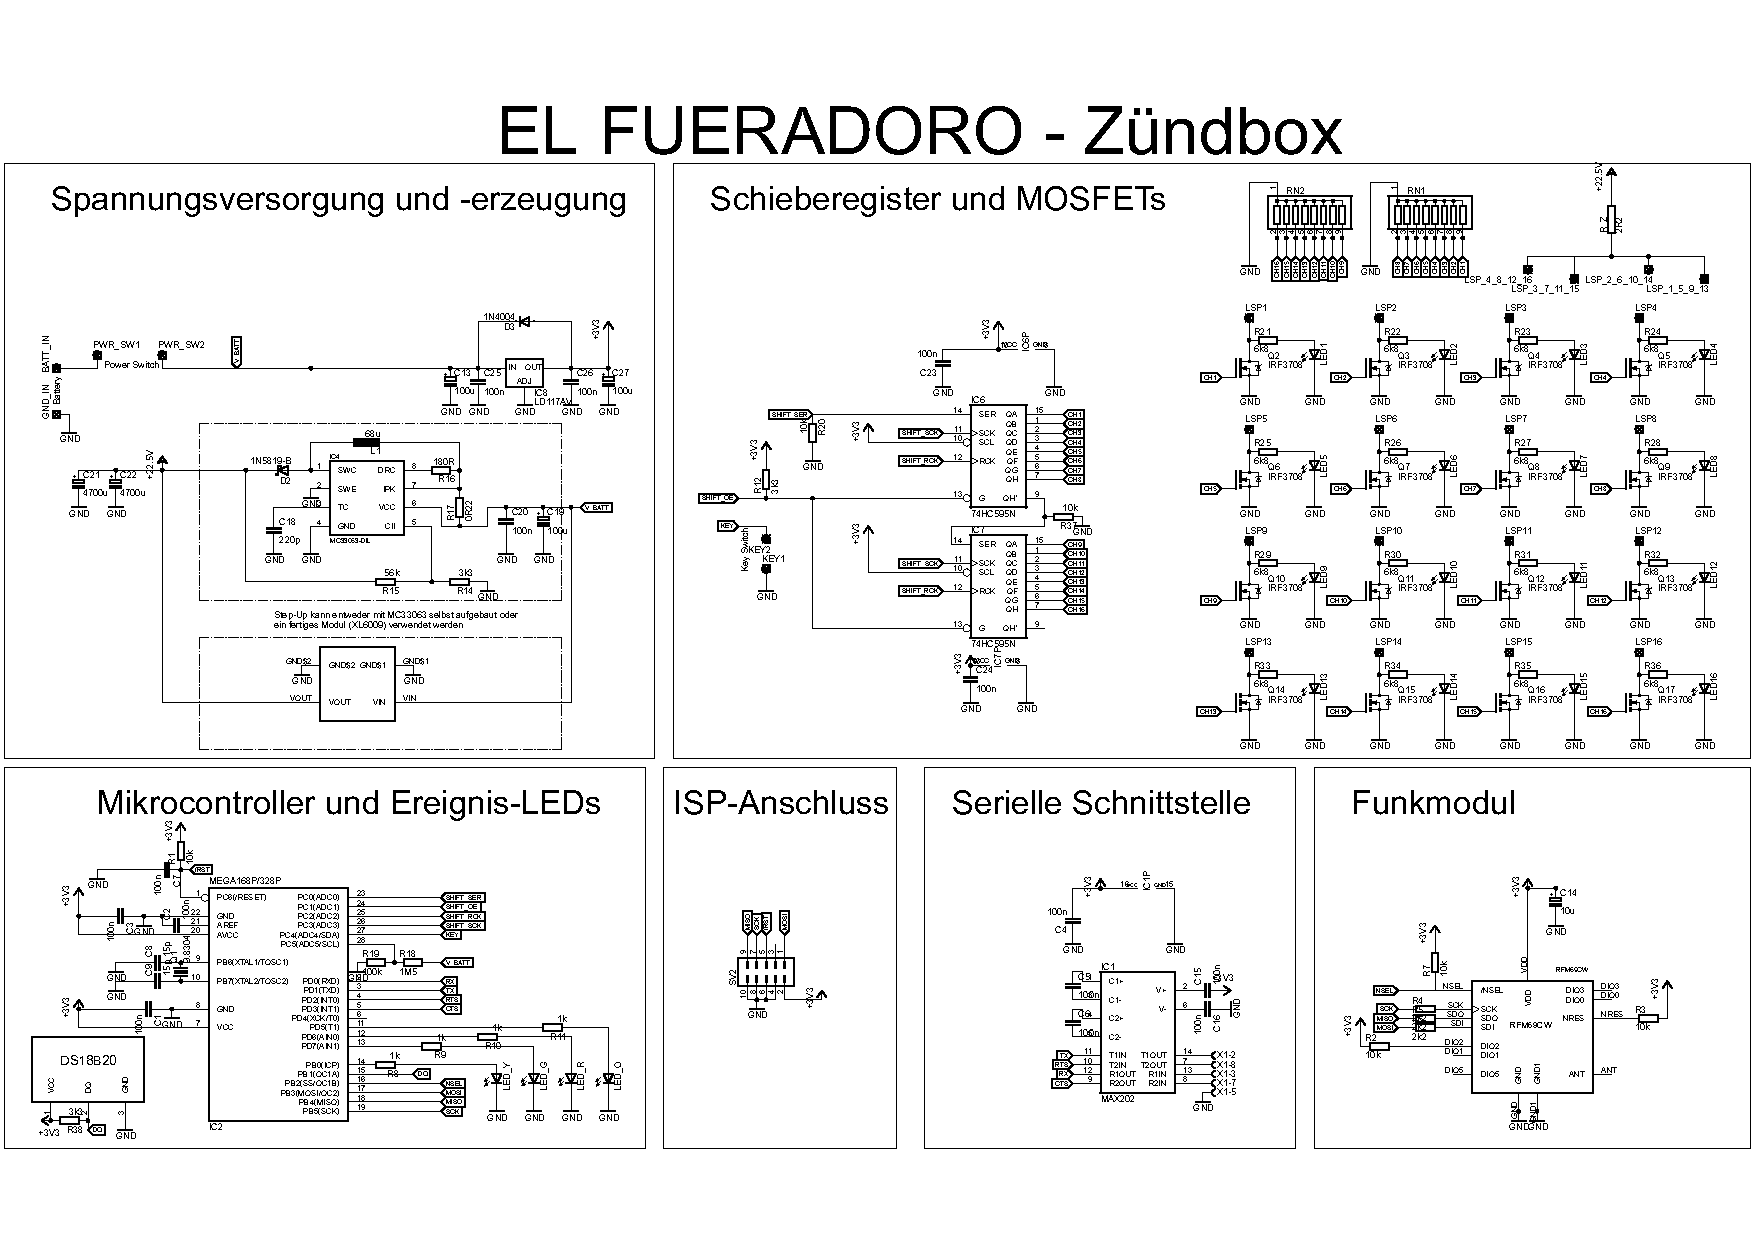
\includegraphics[angle=90, height=.95\textheight,keepaspectratio]{Bilder/Zuendboxschaltplan}
				\caption{Schaltplan der Zündbox}
				\label{fig:zuendboxschematic}
			\end{figure}

			\begin{figure}
				\centering
				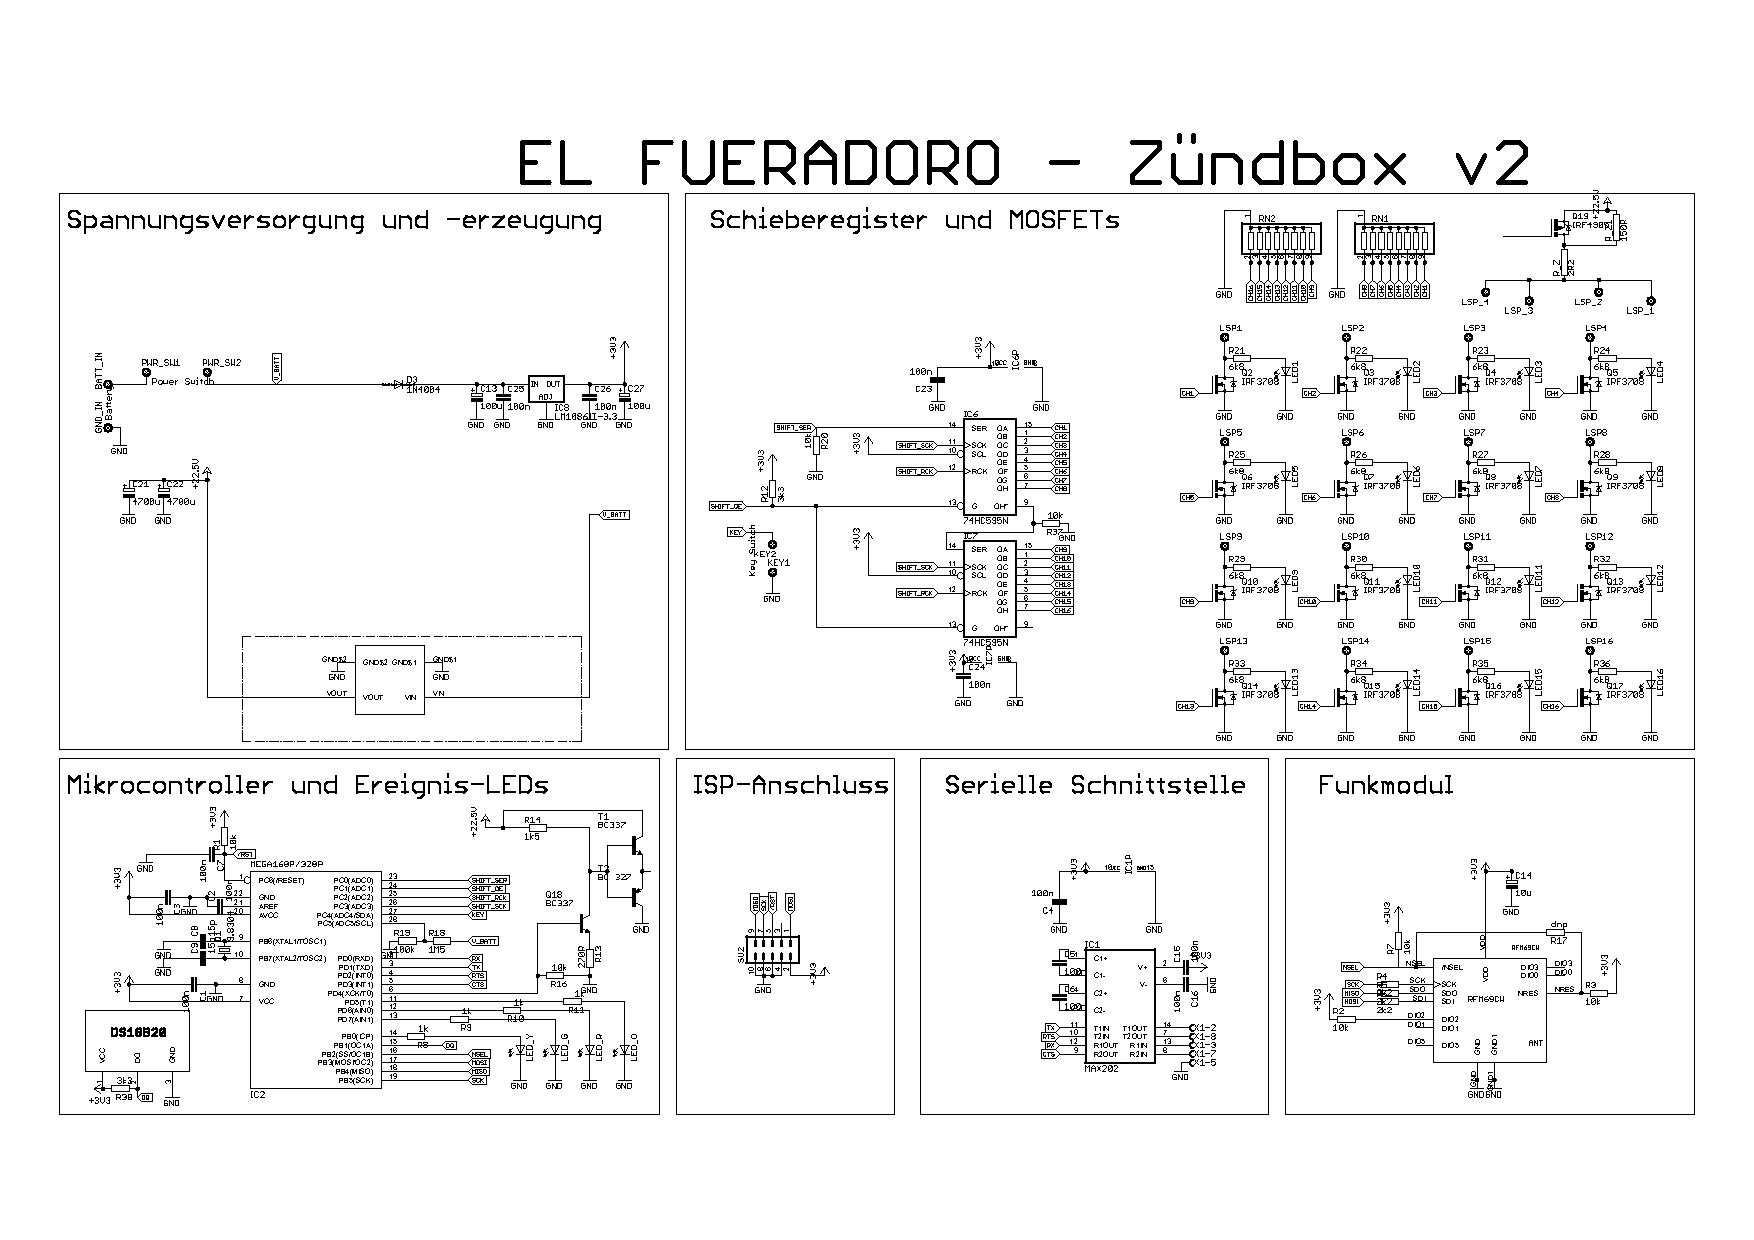
\includegraphics[angle=-90,totalheight=.95\textheight,keepaspectratio]{Bilder/Zuendboxschaltplan2}
				\caption{Schaltplan der Zündbox (2. Generation)}
				\label{fig:zuendbox2schematic}
			\end{figure}

			\begin{figure}
				\centering
				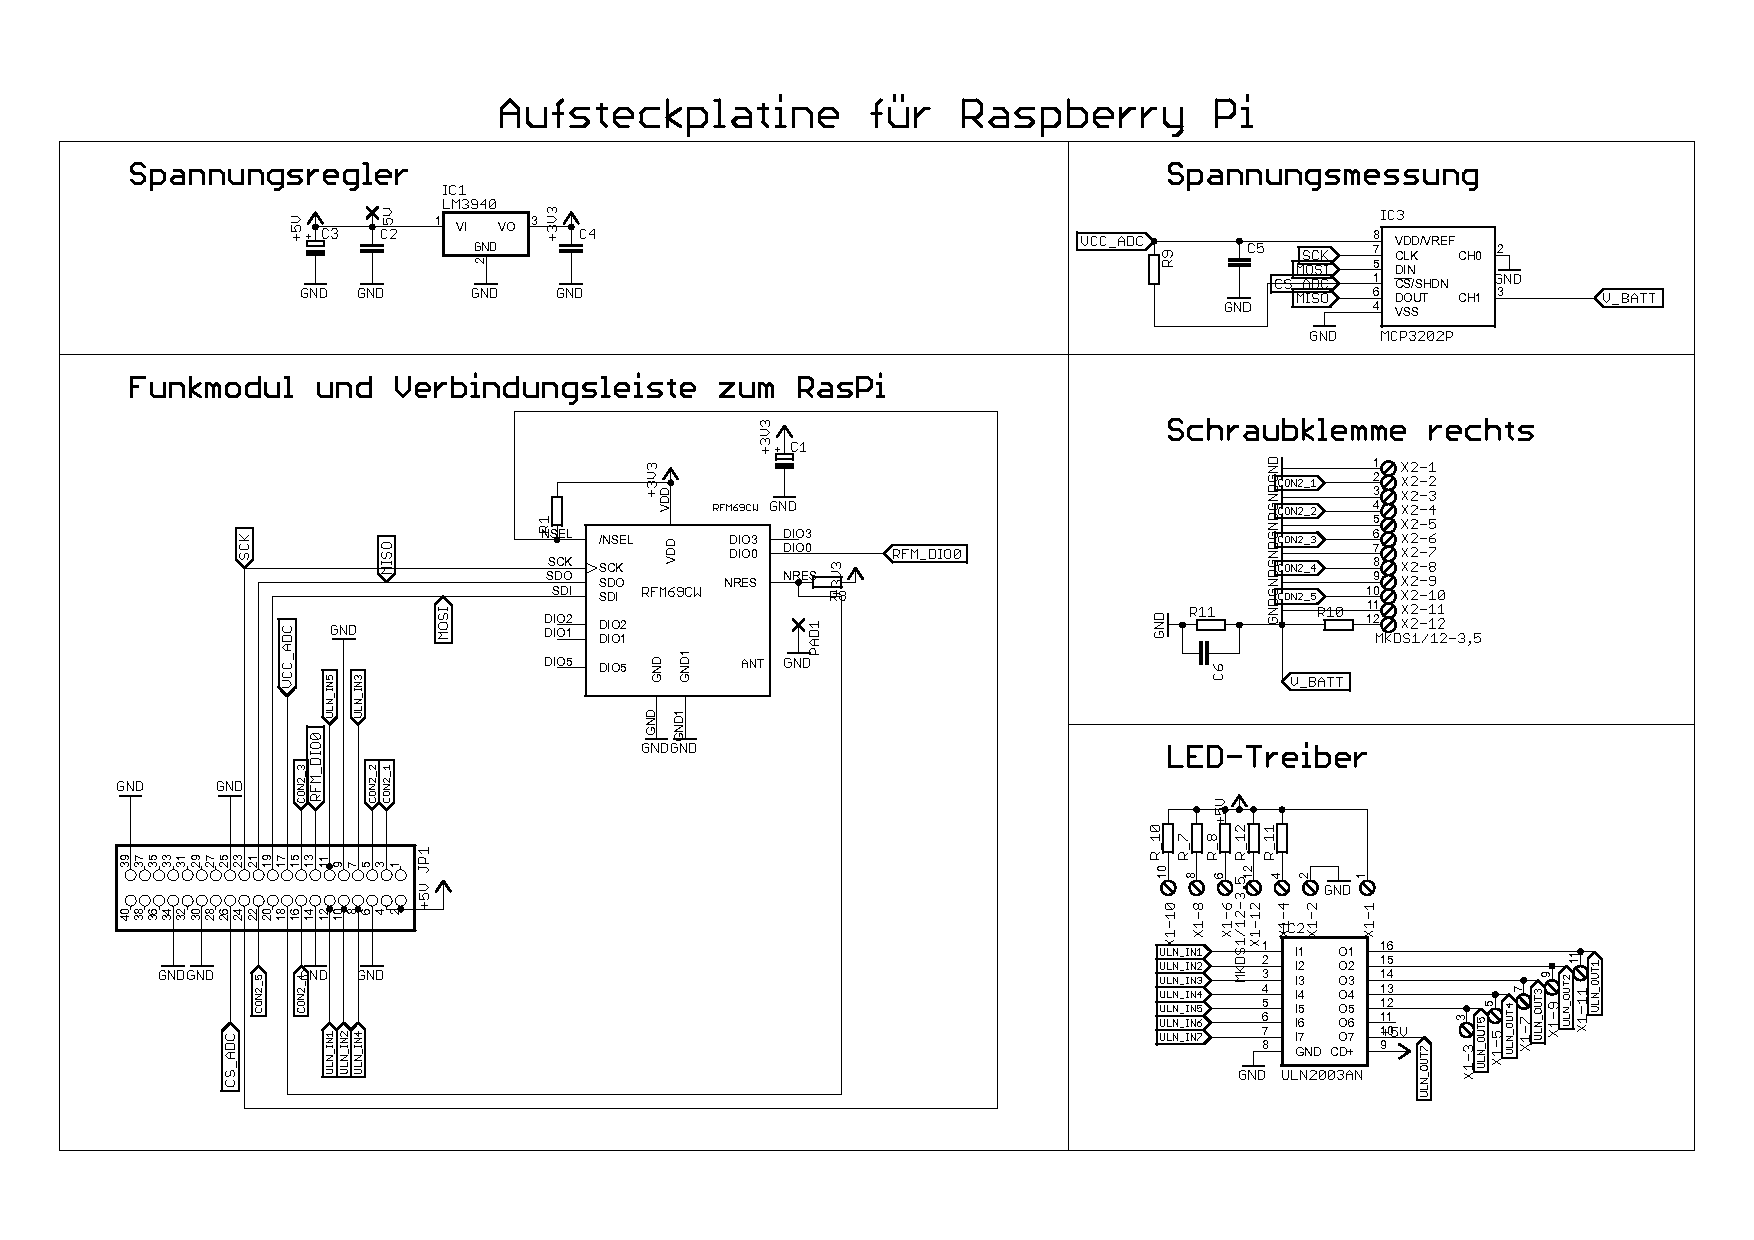
\includegraphics[angle=90,totalheight=.95\textheight,keepaspectratio]{Bilder/Piadapterschaltplan}
				\caption{Schaltplan des Raspberry-Pi-Adapters}
				\label{fig:piadapterschematic}
			\end{figure}

			\begin{figure}
				\centering
				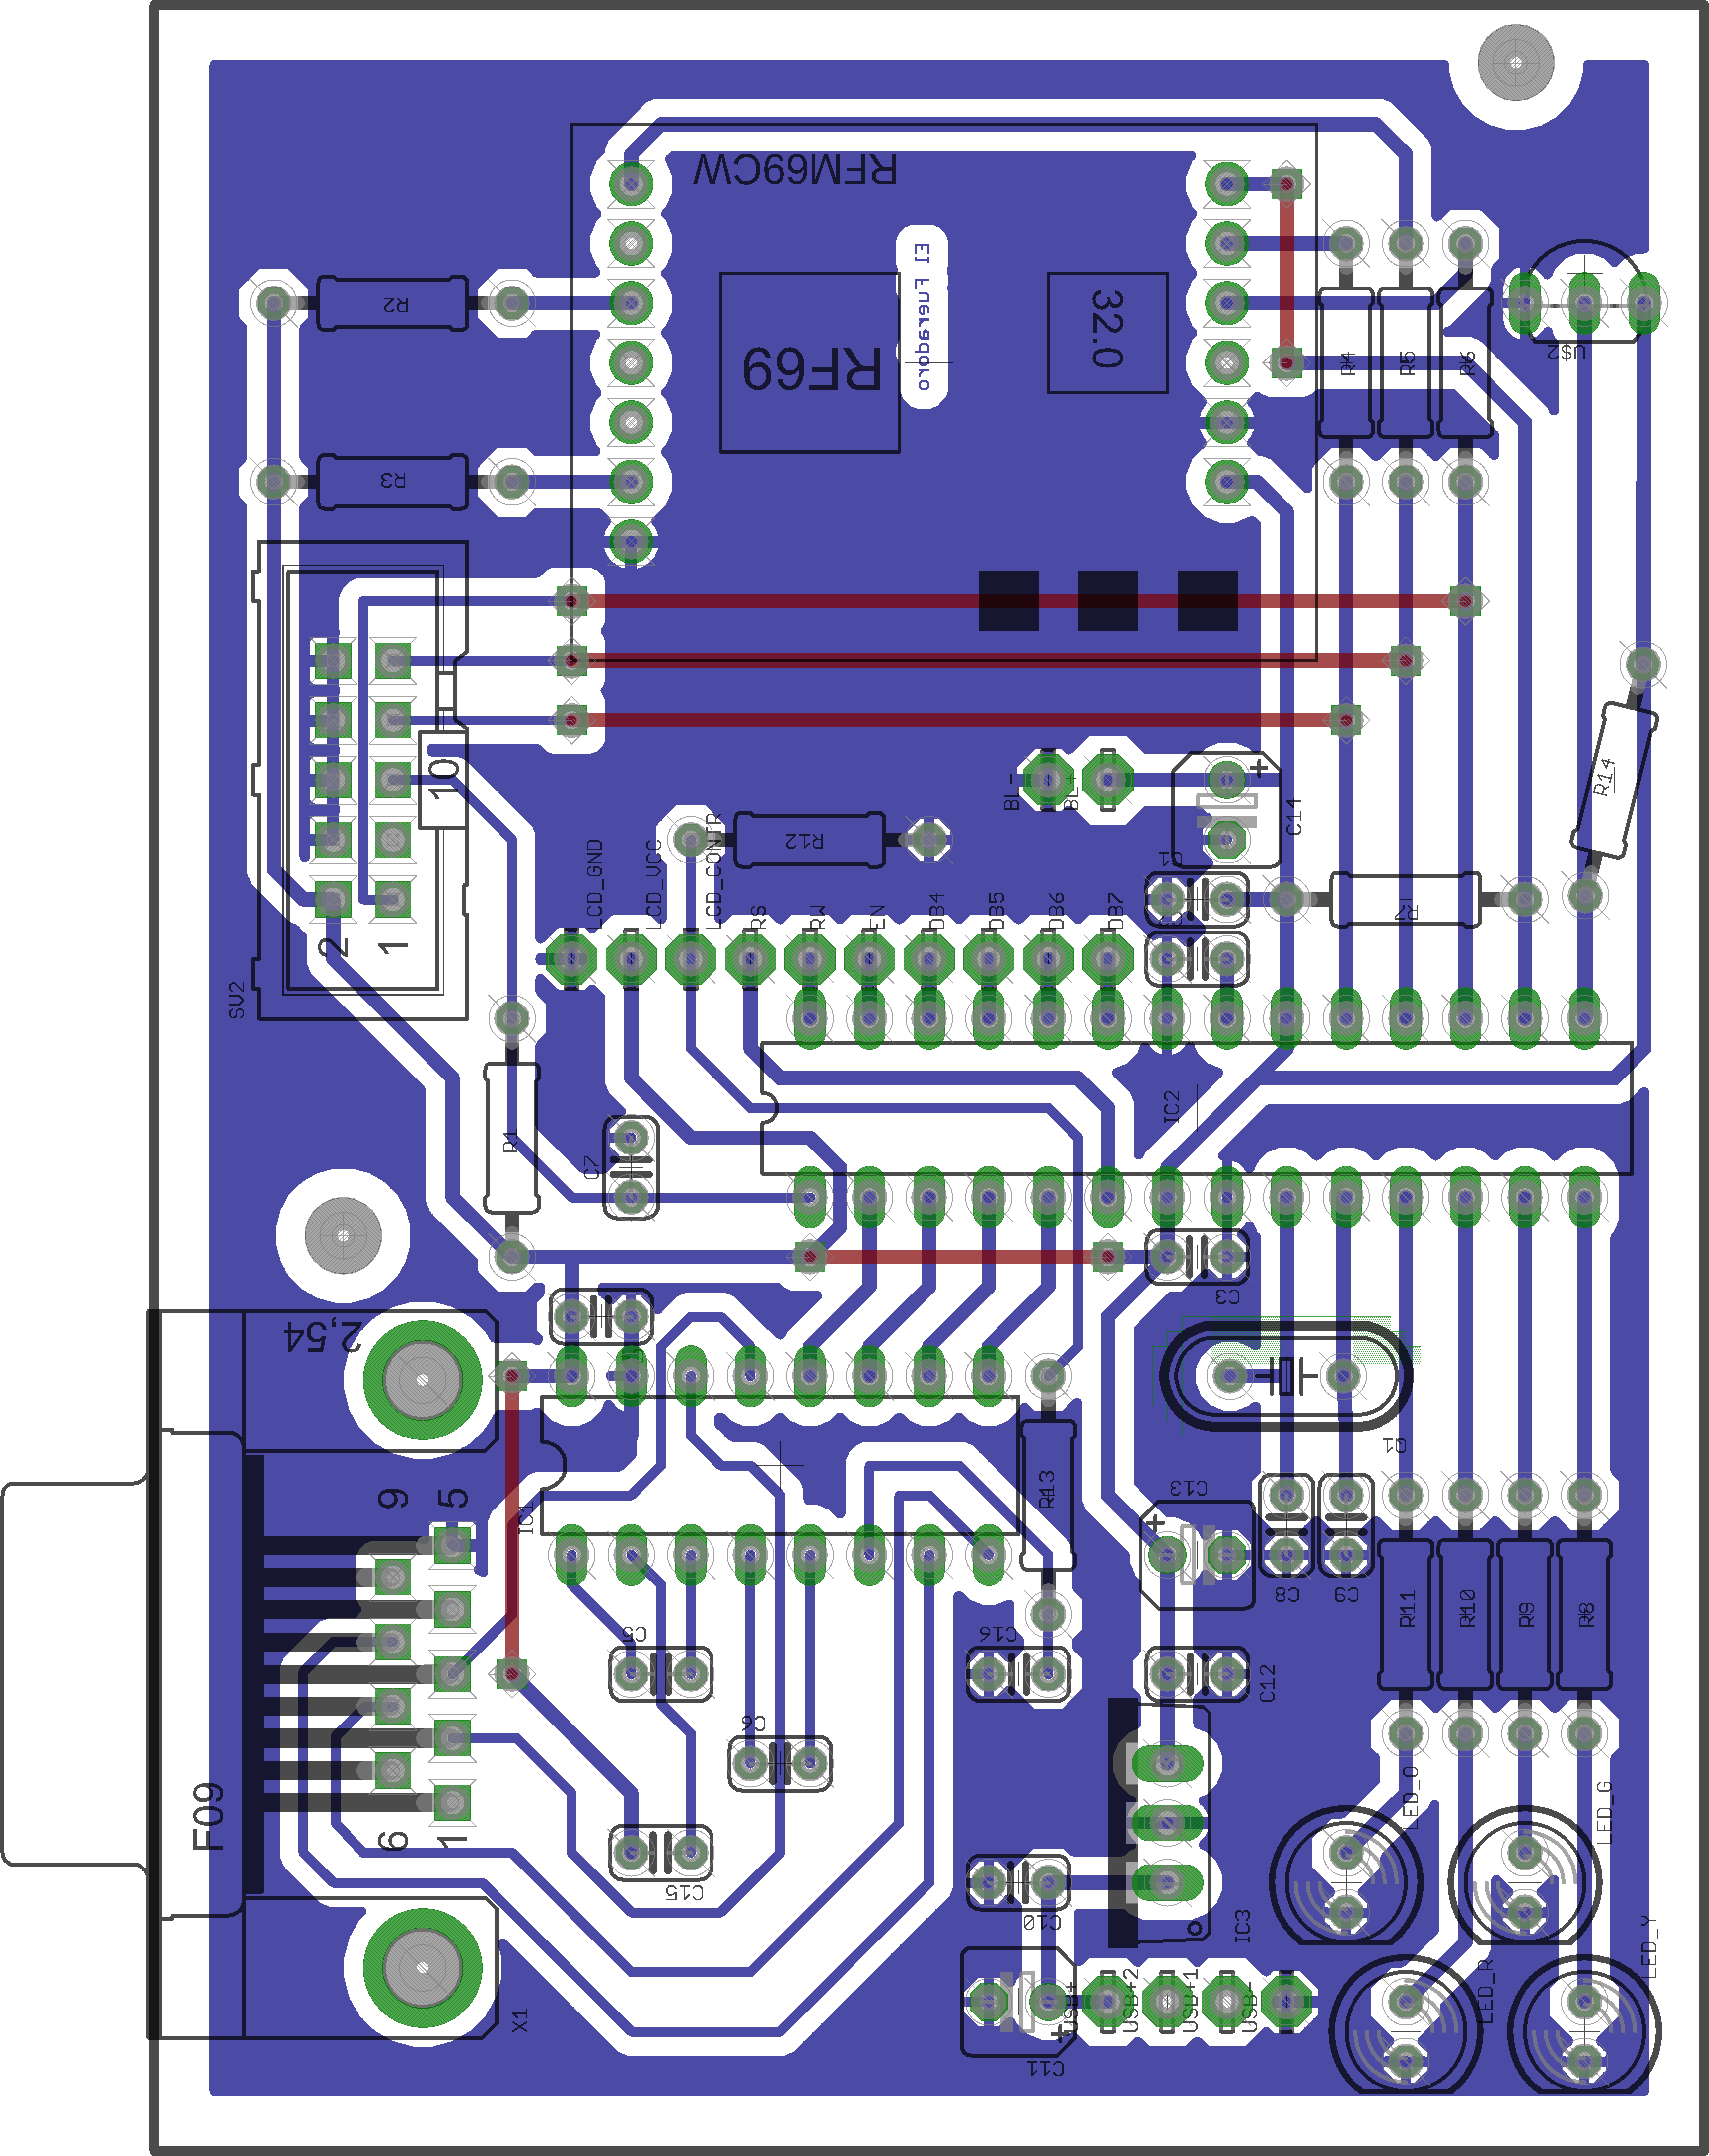
\includegraphics[width=.95\textwidth, keepaspectratio]{Bilder/Transmitterlayout}
				\caption{Layout des Transmitters (keine Originalgröße!)}
				\label{fig:transmitterlayout}
			\end{figure}

			\begin{figure}
				\centering
				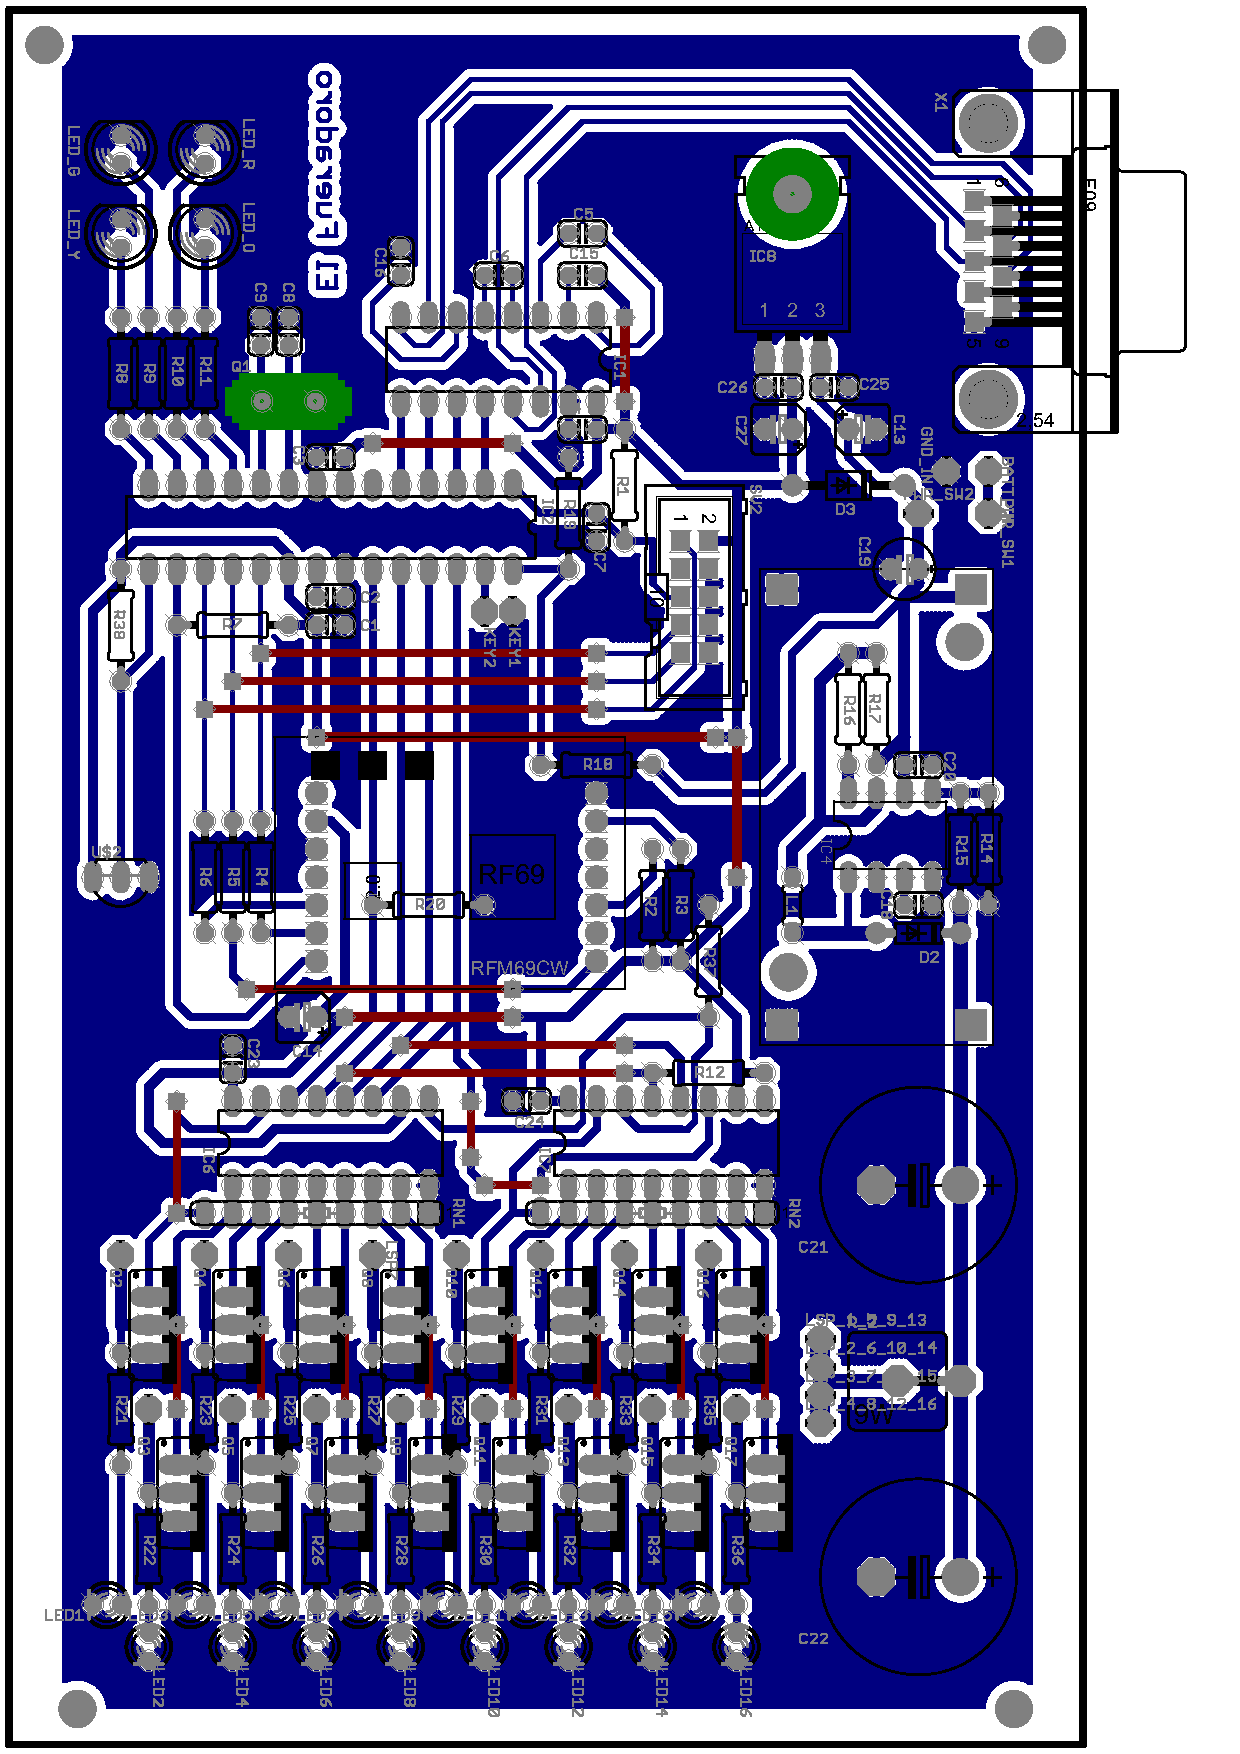
\includegraphics[height=.95\textheight,keepaspectratio]{Bilder/Zuendboxlayout}
				\caption{Layout der Zündbox (keine Originalgröße!)}
				\label{fig:zuendboxlayout}
			\end{figure}

			\begin{figure}
				\centering
				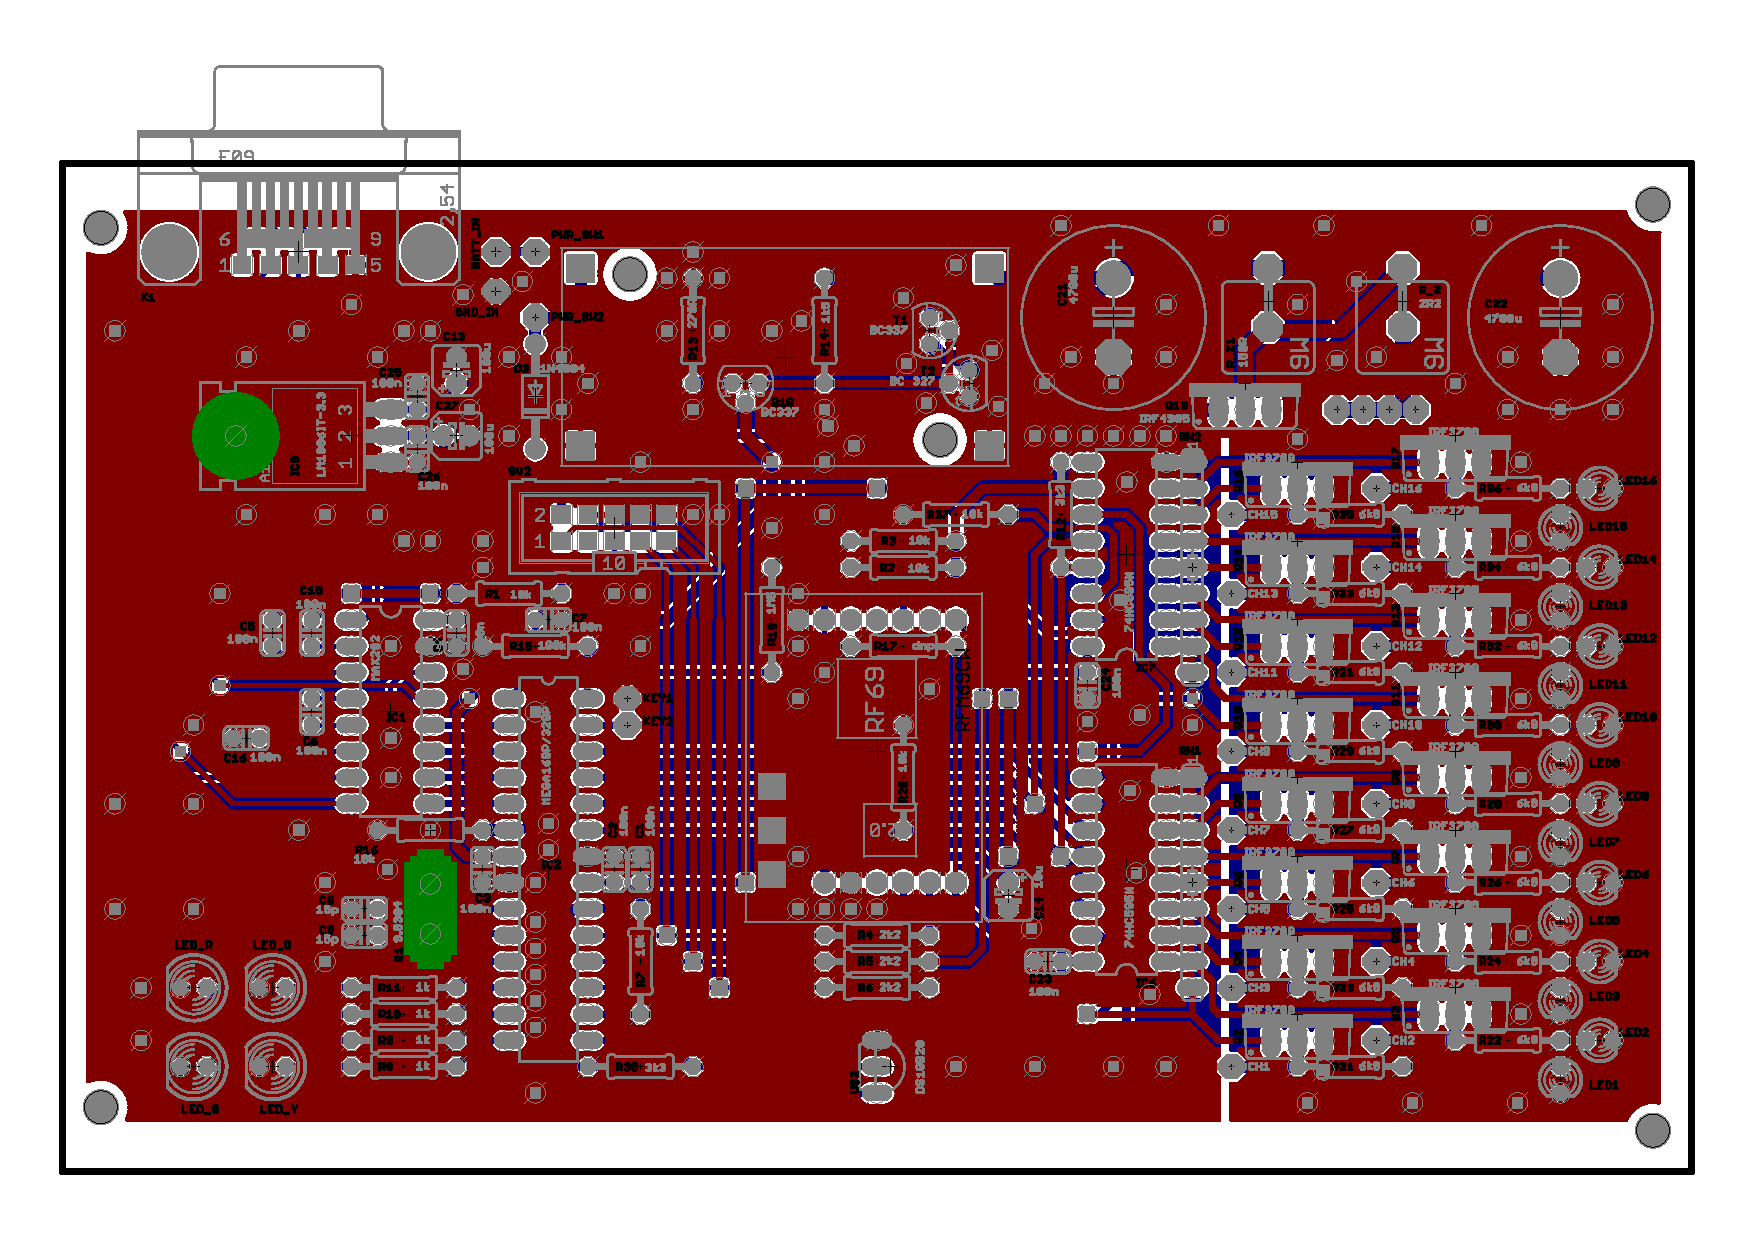
\includegraphics[angle=90, height=.95\textheight,keepaspectratio]{Bilder/Zuendboxlayout2}
				\caption{Layout der Zündbox (2. Generation, keine Originalgröße!)}
				\label{fig:zuendbox2layout}
			\end{figure}

			\begin{figure}
				\centering
				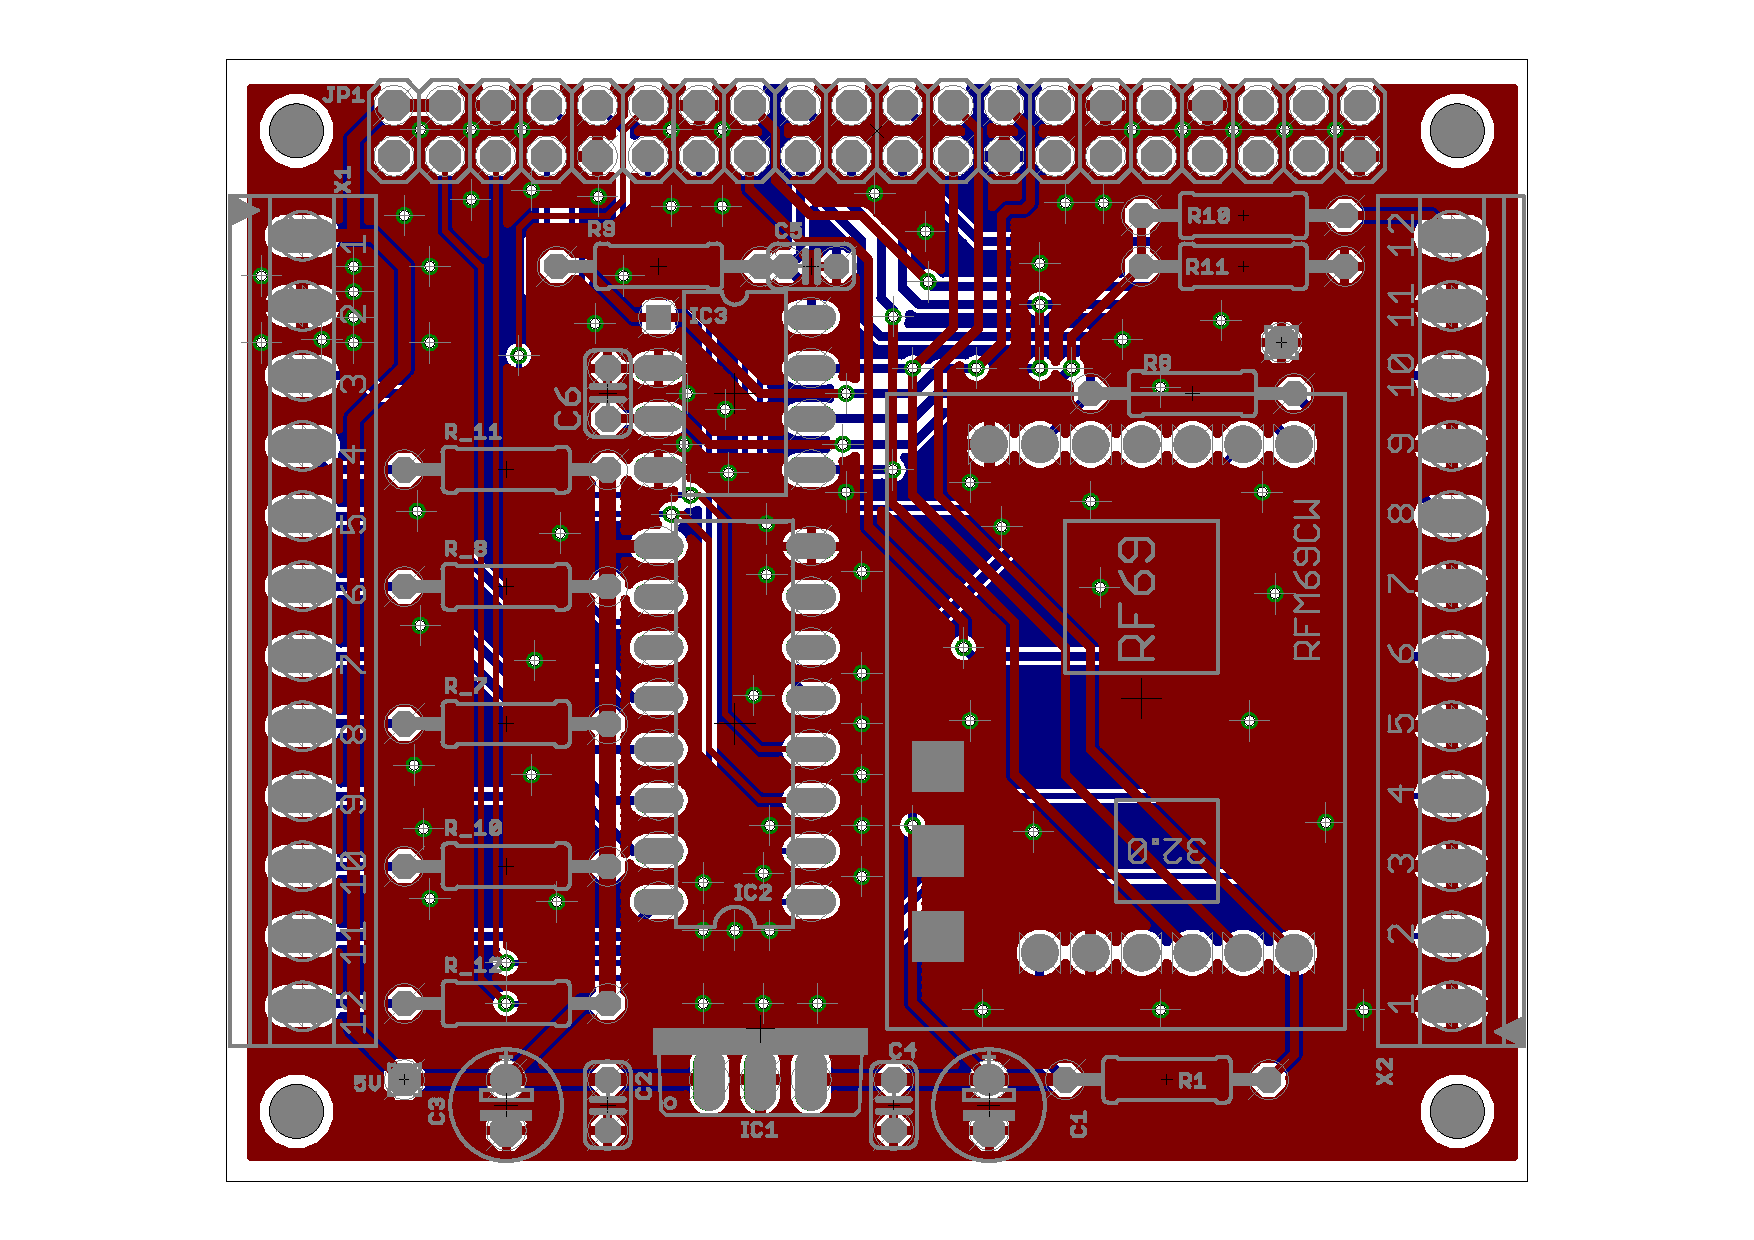
\includegraphics[angle=-90,width=.95\textwidth,keepaspectratio]{Bilder/Piadapterlayout}
				\caption{Layout des Raspberry-Pi-Adapters (keine Originalgröße)}
				\label{fig:piadapterlayout}
			\end{figure}

			\begin{refsection}[bilder/datasheets.bib]
				\newrefcontext[sorting=nty]
				\nocite{*} %Alle Einträge aus .bib anzeigen
				\printbibliography[title=Datenblätter, heading=bibnumbered]
				\label{sec:datasheets}
			\end{refsection}

		\chapter{Pinbelegung}
			\label{ch:pinbelegung}

			\section{Mikrocontroller}
				Die Pinbelegung des \texttt{ATmega328p} in den verschiedenen Devices ist in Abbildung~\ref{fig:pinout} gezeigt.

				\begin{figure}
					\centering
					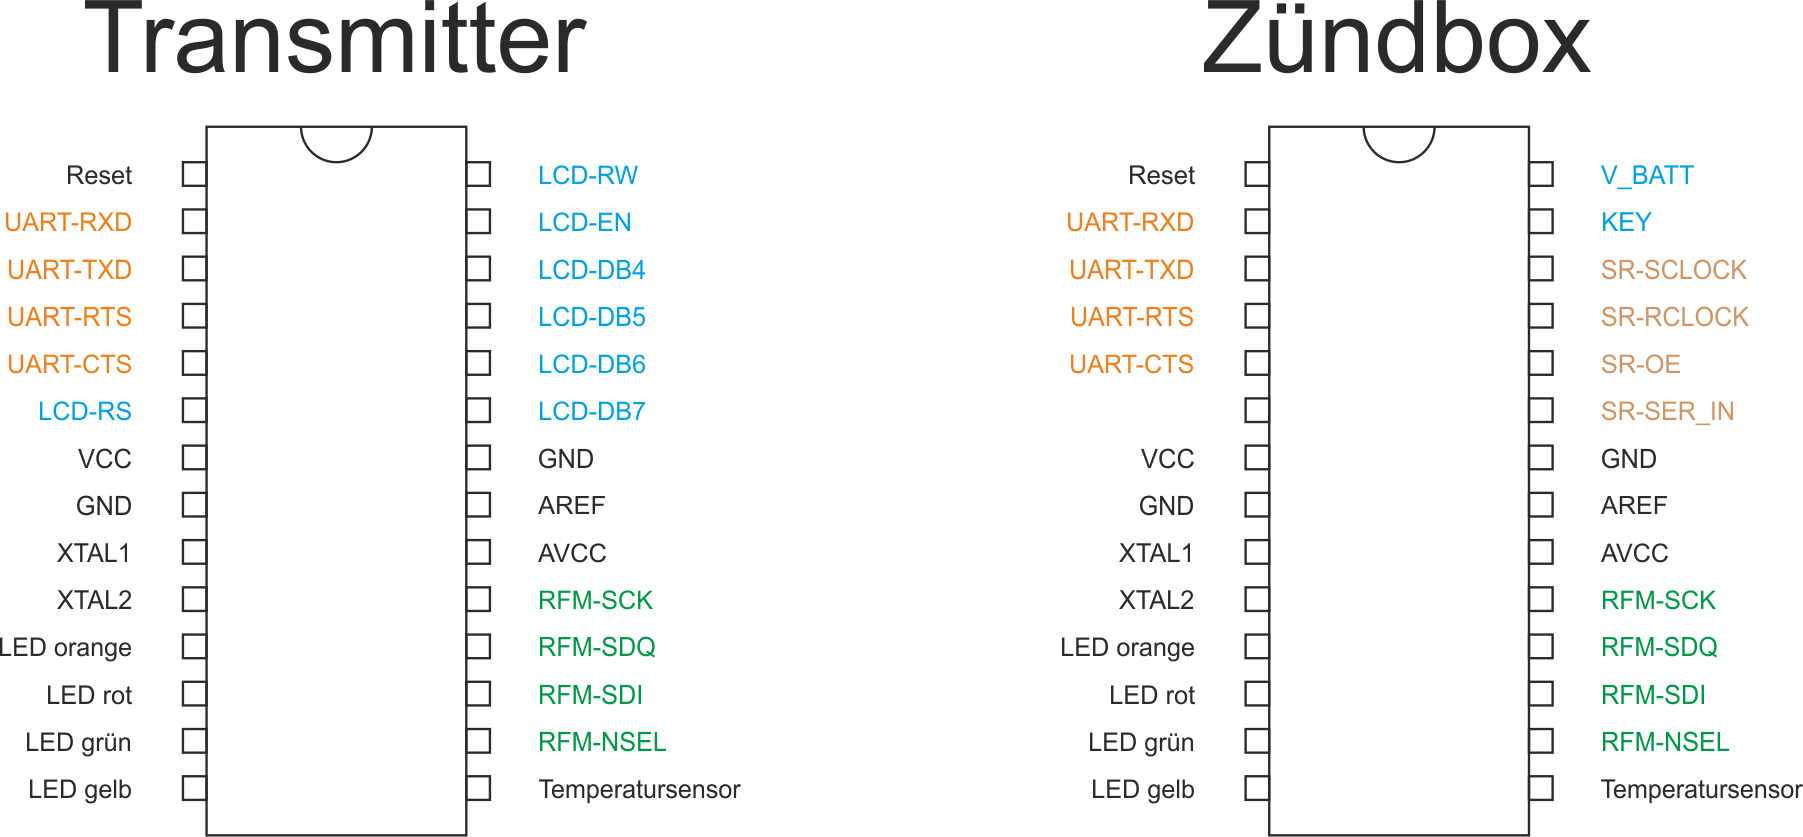
\includegraphics[width=.7\textwidth]{Bilder/pinout}
					\caption{Pinbelegung des Mikrocontrollers bei Transmitter und Zündbox}
					\label{fig:pinout}
				\end{figure}

				Besondere Bedeutung kommt dem Pin rechts oben (LCD-RW bzw. V\_BATT) zu, da er beim Starten der Firmware als Eingang geschaltet wird und aufgrund der dort anliegenden Spannung die sicherheitsrelevante Erkennung, um welchen Devicetyp es sich handelt, vorgenommen wird. Aufgrund eines internen Pullup-Widerstands im LCD werden bei angeschlossenem Transmitter stets $\SI{3,3}{\volt}$ an diesem Pin anliegen, bei Zündboxen bewegt sich die heruntergeteilte Spannung der Versorgungsbatterie im Bereich unterhalb von $\SI{1,1}{\volt}$.

				Diese Unterscheidung ist wichtig, da der Programmablauf sich bei Transmittern (Unique-ID 0 und Slave-ID 0) anders gestaltet als bei Zündboxen und Controllerpins, wie in Abbildung~\ref{fig:pinout} zu sehen, bei Transmittern anders belegt sind und für eine andere Datenrichtung (Eingang/Ausgang) ausgelegt sind als bei Zündboxen.  Wie zu erkennen werden Controlleranschlüsse beim Transmitter als Steuerung des Displays verwendet, die bei der Zündbox den Zustand des Schlüsselschalters einlesen oder die Schieberegister zur Zündung der Kanäle ansteuern.

				Würde die Software beim Start nicht überprüfen, auf welcher Art Device sie gerade läuft, könnte das Programm bei falscher Konfiguration davon ausgehen, auf einem anderen Device zu laufen. Während die Zündbox-Konfiguration auf einem Transmitter~-- abgesehen davon, dass das LCD nichts anzeigen würde~-- keine Probleme hervorriefe, würde es zu Schäden am Controller kommen und zu unerwünschten Zündungen führen, wenn die Transmitter-Konfiguration auf einer Zündbox gestartet werden würde: Im Fall des Schlüsselschalter-Pins käme es  zu einem Kurzschluss, wenn die Box scharf geschaltet ist, was den Controller beschädigen kann, die Ansteuerung des Schieberegisters mit LCD-Befehlen würde dazu führen, dass Zündkanäle durchschalten, weil die Ansteuerbefehle des LCD ans Schieberegister weitergeleitet werden.

				Für den Betrieb der Devices von {\anlage} müssen nicht zwingend die Standardlayouts verwendet werden, die Firmware kann, sofern die Peripherie mit den \enquote{richtigen} Pins verbunden ist, auch auf anderen Boards wie z.\,B. Arduino laufen.

			\section{Raspberry-Pi-Aufsteckplatine}

				Die in Abbildung~\ref{fig:piadapterlayout} gezeigte Platine verfügt über die in den Abbildungen~\ref{fig:piheader} und \ref{fig:piclamps} gezeigte Pinbelegung. Sie ist vom Formfaktor so konzipiert, dass sie mit einer nach unten gerichteten Buchsenleiste auf die Stiftleiste des Raspberry Pi aufgesteckt und an den vier Ecken über insgesamt \SI{11}{\milli\metre} hohe Abstandshalter mit Gewindeschrauben M2,5 mit dem Einplatinencomputer verschraubt werden kann.

				\begin{figure}
					\centering
					\begin{tabularx}{\textwidth}{Xc|cc|cX}
						\cline{3-4}
						Supply            & 3V3  & 1  & 2  & 5V  & Supply             \\
						In 1 (FIRE-Bt.)   & R1   & 3  & 4  & 5V  & Supply             \\
						In 2 (ON/OFF-Bt.) & R2   & 5  & 6  & GND & Supply             \\
						Out 3 (Rx-LED)    & L3   & 7  & 8  & L4  & Out 4 (Tx-LED)     \\
						Supply            & GND  & 9  & 10 & L2  & Out 2 (ON/OFF-LED) \\
						Out 5             & L5   & 11 & 12 & L1  & Out 1 (Fire-LED)   \\
						DIO0 RFM69        & DIO0 & 13 & 14 & GND & Supply             \\
						In 3              & R3   & 15 & 16 & R4  & In 4               \\
						Supply            & 3V3  & 17 & 18 & RES & Reset RFM69        \\
						SPI Master Out    & MOSI & 19 & 20 & GND & Supply             \\
						SPI Slave Out     & MISO & 21 & 22 & R5  & In 5               \\
						SPI Clock         & SCLK & 23 & 24 & CS0 & SPI Select RFM     \\
						Supply            & GND  & 25 & 26 & CS1 & SPI Select ADC     \\
						~                 &      & 27 & 28 &     &                    \\
						~                 &      & 29 & 30 & GND & Supply             \\
						~                 &      & 31 & 32 &     &                    \\
						~                 &      & 33 & 34 & GND & Supply             \\
						~                 &      & 35 & 36 &     &                    \\
						~                 &      & 37 & 38 &     &                    \\
						Supply            & GND  & 39 & 40 &     &                    \\ \cline{3-4}
					\end{tabularx}
					\caption{Belegung Verbindungsstiftleiste Pi-Aufsteckplatine}
					\label{fig:piheader}
				\end{figure}

				Die an den Seiten der Aufsteckplatine angebrachten Schraubklemmen dienen dem Anschluss der am Gehäuse verbauten Indikatoren (LEDs) und Schalterelemente. Welches Signal an welcher Stelle anzuklemmen ist, illustriert Abbildung~\ref{fig:piclamps}, welche eine Draufsicht auf die Oberseite der Aufsteckplatine zeigt.

				Die 40-polige Buchsenleiste zeigt dabei in die Papierebene hinein, die Klemmen an der Seite aus der Papierebene heraus.

				\begin{figure}
					\centering
					\begin{tabularx}{.85\textwidth}{|*{20}{@{}>{\centering\arraybackslash}X@{}}|}
						\hline
						2 & 4 & 6 & 8 & 10 & 12 & 14 & 16 & 18 & 20 & 22 & 24 & 26 & 28 & 30 & 32 & 34 & 36 & 38 & 40 \\
						1 & 3 & 5 & 7 & 9  & 11 & 13 & 15 & 17 & 19 & 21 & 23 & 25 & 27 & 29 & 31 & 33 & 35 & 37 & 39 \\ \hline
					\end{tabularx}
					\vspace{1cm}
					\centering
					\begin{tabularx}{\textwidth}{|r|clXrc|l|}
						\cline{1-1}\cline{7-7}
						1  & U+  & \multirow{2}{*}{U\textsubscript{Force}} &  & \multirow{2}{*}{U\textsubscript{Sense}} & U+     & 1  \\
						2  & GND &                                         &  &                                         & GND    & 2  \\
						3  & -   & \multirow{2}{*}{L5 (Pin 11)}            &  & \multirow{2}{*}{R5}                     & Pin 22 & 3  \\
						4  & +   &                                         &  &                                         & GND    & 4  \\
						5  & -   & \multirow{2}{*}{L4 (Pin 8) TX-LED}      &  & \multirow{2}{*}{R4}                     & Pin 16 & 5  \\
						6  & +   &                                         &  &                                         & GND    & 6  \\
						7  & -   & \multirow{2}{*}{L3 (Pin 7) RX-LED}      &  & \multirow{2}{*}{KEY-Sw. R3}             & Pin 15 & 7  \\
						8  & +   &                                         &  &                                         & GND    & 8  \\
						9  & -   & \multirow{2}{*}{L2 (Pin 10) ON/OFF-LED} &  & \multirow{2}{*}{ON/OFF-Bt. R2}          & Pin 5  & 9  \\
						10 & +   &                                         &  &                                         & GND    & 10 \\
						11 & -   & \multirow{2}{*}{L1 (Pin 12) FIRE-LED}   &  & \multirow{2}{*}{FIRE-Bt. R1}            & Pin 3  & 11 \\
						12 & +   &                                         &  &                                         & GND    & 12 \\ \cline{1-1}\cline{7-7}
					\end{tabularx}
					\caption{Pinbelegung der Aufsteckplatine von oben gesehen}
					\label{fig:piclamps}
				\end{figure}

		\chapter{Software}

			Die Steuerungssoftware für {\anlage} ist unter Zuhilfename des \texttt{AVR-GCC} in der Programmiersprache \texttt{C} geschrieben. Sie umfasst insgesamt 15 Sourcefiles (.c) mit zugehörigen Headerdateien (.h), eine Headerdatei zur Generierung von Registeradressen \enquote{portmakros.h} sowie eine globale Headerdatei \enquote{global.h}, in welcher alle anderen erfasst sind.

			Die Quellcodedateien und ihre Aufgaben sind in Tabelle~\ref{tab:sourcefiles} aufgelistet.

			\begin{table}[h]
				\centering
				\begin{tabular}{lp{125mm}}
					\hline\hline \textbf{Dateiname} & \textbf{Aufgabe(n)}                                                                                                        \\ \hline
					pyro.c                          & Hauptprogramm, Interruptroutinen und anlagenspezifische Funktionen (Schalterinitialisierung, spezielle LCD-Symbole, \dots) \\
					1wire.c                         & Steuerung des Temperatursensors \texttt{DS18B20}                                                                           \\
					adc.c                           & Erfassung der Versorgungsspannung und des Devicetyps mittels Analog-Digital-Converter                                      \\
					addresses.c                     & Unique- und Slave-ID aus dem Speicher holen, speichern, überprüfen                                                         \\
					crcchk.c                        & Überprüfen der Korrektheit empfangener Zeichenketten                                                                       \\
					eeprom.c                        & Direkter Zugriff auf den EEPROM des Controllers                                                                            \\
					lcd.c                           & Steuerung des LCD                                                                                                          \\
					leds.c                          & Kontrolle der vier Status-LEDs                                                                                             \\
					rfm69.c                         & Funktionen für das Funkmodul \texttt{RFM69CW}                                                                              \\
					shiftregister.c                 & Schieberegister-Initialisierung und -Datenübertragung                                                                      \\
					terminal.c                      & \enquote{GUI} zur Benutzerinteraktion via Terminalprogramm                                                                 \\
					timer.c                         & Funktionen zur Timer-Steuerung                                                                                             \\
					uart.c                          & Kommunikation über serielle Schnittstelle                                                                                  \\ \hline\hline
				\end{tabular}
				\caption{Quellcodedateien und ihre Funktionen}
				\label{tab:sourcefiles}
			\end{table}

	\part{Aufbauanleitung}
		\label{part:aufbauanleitung}

		\chapter{Materiallisten}

			In den Tabellen dieses Kapitels sind die benötigten Teile für den Aufbau der verschiedenen Devices von {\anlage} zusammen mit möglichen Bezugsquellen und Preisen (Stand Januar 2015, teils aktualisiert im August 2015) aufgelistet. Bei den Zündboxen wird die zweite Generation empfohlen, die zusätzliche Sicherheit gegenüber der ersten Generation bietet. Es ist jedoch problemlos möglich, beide Generationen gemeinsam in einer Show zu verwenden.

			Leider ist es~-- schon alleine aufgrund der Währungsschwankungen, denen besonders die eBay-Artikel unterworfen sind~-- ein Ding der Unmöglichkeit, die Liste permanent tagesaktuell zu halten. Tote Links dürfen gerne gemeldet werden.

			{\footnotesize
			\begin{longtable}{p{1.2cm}cp{2.5cm}llSSp{2.35cm}}
				\multicolumn{8}{c}{\textbf{Materialliste Transmitter}}                                                                                                                                  \\
				\\ \hline
				Bauteil                        & Anz. & Beschreibung                         & Händler  & Artikelnr.                                                & {Einzel} & {Ges.}  & Bemerkung    \\ [8pt]
				\hline
				\multicolumn{8}{c}{Kondensatoren}                                                                                                                                                       \\
				C11, C13                       & 2    & Elektrolyt\-kon\-den\-sa\-tor, 100uF & Reichelt & RAD 105 100/35                                            & 0,04\,€  & 0,08\,€ &              \\
				C14                            & 1    & Elektrolyt\-kon\-den\-sa\-tor, 10uF  & Reichelt & RAD 10/100                                                & 0,04\,€  & 0,04\,€ &              \\
				C1{\dots}7, C10, C12, C15, C16 & 11   & Keramik\-kon\-den\-sator, 100nF      & Reichelt & X7R-2,5 100N                                              & 0,04\,€  & 0,44\,€ &              \\
				C8, C9                         & 2    & Keramik\-kon\-den\-sator, 15pF       & Reichelt & KERKO 15P                                                 & 0,05\,€  & 0,10\,€ &              \\ [8pt]
				\hline
				\multicolumn{8}{c}{Integrierte Schaltungen}                                                                                                                                             \\
				IC2                            & 1    & ATMEGA 328P                          & Reichelt & ATMEGA 328P-PU                                            & 2,65\,€  & 2,65\,€ &              \\
				IC1                            & 1    & MAX202                               & Reichelt & MAX 202 ECPE                                              & 1,40\,€  & 1,40\,€ &              \\
				U\$4                           & 1    & RFM69CW                              & Pollin   & 810 303                                                   & 4,60\,€  & 4,60\,€ &              \\
				U\$2                           & 1    & DS18B20                              & Reichelt & DS 18B20                                                  & 1,60\,€  & 1,60\,€ &              \\
				IC8                            & 1    & LM3940-3,3                           & Reichelt & LM 3940 IT3,3                                             & 1,10\,€  & 1,10\,€ &              \\ [8pt]
				\hline
				\multicolumn{8}{c}{Display}                                                                                                                                                             \\
				                               & 1    & LCD, 20x4 Zeichen, HD44780-komp.     & eBay     & \href{http://www.ebay.com/itm/291548935509}{291548935509} & 4,80\,€  & 4,80\,€ &              \\ [8pt]
				\hline
				\multicolumn{8}{c}{LEDs}                                                                                                                                                                \\
				LED\_O                         & 1    & LED, 5mm, orange                     & Reichelt & LED 5MM R OR                                              & 0,12\,€  & 0,12\,€ &              \\
				LED\_R                         & 1    & LED, 5mm, rot                        & Reichelt & LED 5MM RT                                                & 0,06\,€  & 0,06\,€ &              \\
				LED\_Y                         & 1    & LED, 5mm, gelb                       & Reichelt & LED 5MM GE                                                & 0,06\,€  & 0,06\,€ &              \\
				LED\_G                         & 1    & LED, 5mm, grün                       & Reichelt & LED 5MM GN                                                & 0,06\,€  & 0,06\,€ &              \\ [8pt]
				\hline
				\multicolumn{8}{c}{Quarz}                                                                                                                                                               \\ \nopagebreak
				Q1                             & 1    & Standardquarz, Grundton, 9,8304 Mhz  & Reichelt & 9,8304-HC49U-S                                            & 0,15\,€  & 0,15\,€ &              \\ [8pt]
				\hline
				\multicolumn{8}{c}{Widerstände}                                                                                                                                                         \\
				R13                            & 1    & 6k8                                  & Reichelt & 1/4W 6,8K                                                 & 0,08\,€  & 0,08\,€ &              \\
				R12, R14                       & 2    & 3k3                                  & Reichelt & METALL 3,30K                                              & 0,08\,€  & 0,16\,€ &              \\
				R1, R2, R3, R7                 & 4    & 10k                                  & Reichelt & METALL 10,0K                                              & 0,08\,€  & 0,33\,€ &              \\
				R4{\dots}6, R8{\dots}11        & 7    & 1k0                                  & Reichelt & METALL 1,00K                                              & 0,08\,€  & 0,57\,€ & 10 billiger! \\ [8pt]
				\hline
				\multicolumn{8}{c}{Mechanische Bauteile}                                                                                                                                                \\
				X1                             & 1    & Sub-D-Buchse, 9-pol                  & Reichelt & D-SUB BU 09US                                             & 0,23\,€  & 0,23\,€ &              \\
				SV2                            & 1    & Wannenstecker, 10-pol                & Reichelt & WSL 10G                                                   & 0,08\,€  & 0,08\,€ &              \\
				                               & 1    & Box                                  & Reichelt & GEH KS 50                                                 & 2,65\,€  & 2,65\,€ &              \\
				                               & 1    & USB-Kabel als Stromkabel             & Reichelt & AK 670/2-1,0                                              & 0,70\,€  & 0,70\,€ &              \\ [8pt]
				\hline
				\multicolumn{8}{c}{HF-Komponenten}                                                                                                                                                      \\
				                               & 1    & SMA-Kabel Funkmodul-Gehäuse          & eBay     & \href{http://www.ebay.com/itm/161134814025}{161134814025} & 2,53\,€  & 2,53\,€ &              \\
				                               & 1    & Antenne 868 MHz                      & eBay     & \href{http://www.ebay.de/itm/380436601891}{380436601891}  & 4,24\,€  & 4,24\,€ &              \\
				                               & 1    & SMA-Platinenbuchse, 1,6mm            & eBay     & \href{http://www.ebay.com/itm/220952712009}{220952712009} & 1,17\,€  & 1,17\,€ &              \\ \hline
				\caption{\normalsize Materialliste für den Transmitter}
				\label{tab:transmitterbom}
			\end{longtable}
			}

			\newpage

			{\footnotesize
				\begin{longtable}{p{1.2cm}cp{2.5cm}llSSp{2.35cm}}
					\multicolumn{8}{c}{\textbf{Materialliste Raspberry-Pi-Transmitter}}                                                                                                                                                                                                                                                          \\
					\\ \hline
					Bauteil           & Anz. & Beschreibung                                          & Händler    & Artikelnr.                                                                                                                                                  & {Einzel} & {Ges.}   & Bemerkung                                \\ [8pt]
					\hline
					\multicolumn{8}{c}{Kondensatoren}                                                                                                                                                                                                                                                                                            \\
					C1, C3            & 2    & Elektrolyt\-kon\-den\-sa\-tor, 10uF                   & Reichelt   & RAD 10/100                                                                                                                                                  & 0,04\,€  & 0,08\,€  &                                          \\
					C2, C4, C5, C6    & 4    & Keramik\-kon\-den\-sator, 100nF                       & Reichelt   & X7R-2,5 100N                                                                                                                                                & 0,04\,€  & 0,12\,€  &                                          \\ [8pt]
					\hline
					\multicolumn{8}{c}{Integrierte Schaltungen}                                                                                                                                                                                                                                                                                  \\
					IC1               & 1    & LM3940-3,3                                            & Reichelt   & LM 3940 IT3,3                                                                                                                                               & 1,10\,€  & 1,10\,€  &                                          \\
					IC2               & 1    & ULN2003A                                              & Reichelt   & ULN 2003A                                                                                                                                                   & 0,29\,€  & 0,29\,€  &                                          \\
					IC3               & 1    & MCP3202-CI/P                                          & eBay       & \href{http://www.ebay.com/itm/250878853097}{250878853097}                                                                                                   & 4,20\,€  & 4,20\,€  &                                          \\
					                  & 1    & RFM69CW                                               & Pollin     & 810 303                                                                                                                                                     & 4,60\,€  & 4,60\,€  &                                          \\ [8pt]
					\hline
					\multicolumn{8}{c}{Einplatinenrechner und Zubehör}                                                                                                                                                                                                                                                                           \\
					                  & 1    & Raspberry Pi 3                                        & Reichelt   & RASPBERRY PI 3                                                                                                                                              & 37,50\,€ & 37,50\,€ &                                          \\
					                  & 1    & Micro-SD-Speicherkarte, 16\,GB                        & Reichelt   & INTENSO 3433470                                                                                                                                             & 9,95\,€  & 9,95\,€  &                                          \\
					                  & 1    & Waveshare 7 inch 1024*600 Capacitive Touch Screen LCD & Amazon     & \href{http://www.amazon.de/gp/product/B015E8EDYQ}{B015E8EDYQ}                                                                                               & 58,99\,€ & 58,99\,€ &                                          \\
					                  & 1    & USB-Soundkarte                                        & Amazon     & \href{https://www.amazon.de/gp/product/B00C7LXUDY}{B00C7LXUDY}                                                                                              & 6,25\,€  & 6,25\,€  &                                          \\
					                  & 1    & Powerbank                                             & Amazon     & \href{https://www.amazon.de/B01KPFC4B2}{B01KPFC4B2}                                                                                                         & 20,89\,€ & 20,89\,€ &                                          \\
					                  & 1    & Waveshare 7 inch 1024*600 Capacitive Touch Screen LCD & Amazon     & \href{http://www.amazon.de/gp/product/B015E8EDYQ}{B015E8EDYQ}                                                                                               & 58,99\,€ & 58,99\,€ &                                          \\ [8pt]
					\hline
					\multicolumn{8}{c}{LEDs}                                                                                                                                                                                                                                                                                                     \\
					LED\_O            & 1    & LED, 5mm, orange                                      & Reichelt   & LED 5MM R OR                                                                                                                                                & 0,12\,€  & 0,12\,€  &                                          \\
					LED\_G            & 1    & LED, 5mm, grün                                        & Reichelt   & LED 5MM GN                                                                                                                                                  & 0,06\,€  & 0,06\,€  &                                          \\ [8pt] \hline
					\multicolumn{8}{c}{Taster}                                                                                                                                                                                                                                                                                                   \\
					Taster            & 2    & LED, 5mm, orange                                      & AliExpress & \href{https://www.aliexpress.com/item/Mini-12mm-3V-Momentary-On-Off-Push-Button-Switch-for-Car-Auto-Boat-Circuit-Control-Electrical/32597982325.html}{Link} & 2,42\,€  & 4,84\,€  & Bei Bestellung angeben: 1x rot, 1x blau! \\ [8pt]
					\hline
					\multicolumn{8}{c}{Widerstände}                                                                                                                                                                                                                                                                                              \\
					R\_10             & 1    & 100R                                                  & Reichelt   & METALL 100                                                                                                                                                  & 0,08\,€  & 0,08\,€  &                                          \\
					R\_12             & 1    & 150R                                                  & Reichelt   & METALL 150                                                                                                                                                  & 0,08\,€  & 0,08\,€  &                                          \\
					R1, R8, R9, R10   & 4    & 10k                                                   & Reichelt   & METALL 10,0K                                                                                                                                                & 0,08\,€  & 0,33\,€  &                                          \\
					R11               & 1    & 2k2                                                   & Reichelt   & METALL 2,20K                                                                                                                                                & 0,08\,€  & 0,08\,€  &                                          \\
					R\_7, R\_8, R\_11 & 3    & 1k0                                                   & Reichelt   & METALL 1,00K                                                                                                                                                & 0,08\,€  & 0,24\,€  &                                          \\ [8pt]
					\hline
					\multicolumn{8}{c}{Mechanische Bauteile}                                                                                                                                                                                                                                                                                     \\
					                  & 4    & Schraubklemme, 6-pol                                  & Reichelt   & AKL 059-06                                                                                                                                                  & 0,72\,€  & 2,88\,€  &                                          \\
					                  & 1    & Buchsenleiste, 2x20-pol                               & Pollin     & 451 358                                                                                                                                                     & 0,55\,€  & 0,55\,€  &                                          \\
					                  & 1    & Buchsenleiste mit 6 Plätzen                           & Reichelt   & MPE 094-1-006                                                                                                                                               & 0,25\,€  & 0,25\,€  &                                          \\
					                  & 1    & Buchsenleiste mit 7 Plätzen                           & Reichelt   & MPE 094-1-007                                                                                                                                               & 0,31\,€  & 0,31\,€  &                                          \\
					                  & 1    & Micro-USB-Kabel Powerbank-Pi                          & Reichelt   & DELOCK 83897                                                                                                                                                & 1,25\,€  & 1,25\,€  &                                          \\
					                  & 1    & Micro-USB-Kabel Pi-Touchscreen                        & AliExpress & \href{http://www.aliexpress.com/item/Up-Angled-90-Degree-Micro-USB-Male-to-USB-Data-Charge-Cable-for-I9500-9300-N7100/32266663376.html}{Link}               & 2,53\,€  & 2,53\,€  & Umsetzungs\-abhängig                     \\
					                  & 1    & HDMI-Kabel Pi-Touchscreen                             & eBay       & \href{http://www.ebay.de/itm/361031629625}{361031629625}                                                                                                    & 4,99\,€  & 4,99\,€  & Umsetzungs\-abhängig                     \\ [8pt]
					\hline
					\multicolumn{8}{c}{HF-Komponenten}                                                                                                                                                                                                                                                                                           \\
					                  & 1    & SMA-Kabel Funkmodul-Gehäuse                           & eBay       & \href{http://www.ebay.com/itm/161134814025}{161134814025}                                                                                                   & 2,53\,€  & 2,53\,€  &                                          \\
					                  & 1    & Antenne 868 MHz                                       & eBay       & \href{http://www.ebay.de/itm/380436601891}{380436601891}                                                                                                    & 4,24\,€  & 4,24\,€  &                                          \\
					                  & 1    & SMA-Platinenbuchse, 1,6mm                             & eBay       & \href{http://www.ebay.com/itm/220952712009}{220952712009}                                                                                                   & 1,17\,€  & 1,17\,€  &                                          \\ \hline
					\caption{\normalsize Materialliste für den Raspberry-Pi-Transmitter}
					\label{tab:raspibom}
				\end{longtable}
			}

			\newpage

			{\footnotesize
				\begin{longtable}{p{1.2cm}cp{2.5cm}llSSp{2.35cm}}
					\multicolumn{8}{c}{\textbf{Materialliste Zündbox}}                                                                                                                                                                            \\
					\\
					Bauteil                                 & Anz. & Beschreibung                              & Händler    & Artikelnr.                                                           & {Einzel} & {Ges.}   & Bemerkung              \\
					\hline
					\multicolumn{8}{c}{Kondensatoren}                                                                                                                                                                                             \\
					C13, C27, C19                           & 3    & Elektrolyt\-kon\-den\-sa\-tor, 100uF      & Reichelt   & RAD 105 100/35                                                       & 0,04\,€  & 0,12\,€  &                        \\
					C14                                     & 1    & Elektrolyt\-kon\-den\-sa\-tor, 10uF       & Reichelt   & RAD 10/100                                                           & 0,04\,€  & 0,04\,€  &                        \\
					C21, C22                                & 2    & Elektrolyt\-kon\-den\-sa\-tor, 4700uF 35V & Reichelt   & RAD 4.700/35                                                         & 0,45\,€  & 0,90\,€  &                        \\
					C1{\dots}7, C15, C16, C20, C23{\dots}26 & 14   & Keramik\-kondensator, 100nF               & Reichelt   & X7R-2,5 100N                                                         & 0,04\,€  & 0,56\,€  &                        \\
					C8, C9                                  & 2    & Keramik\-kondensator, 15pF                & Reichelt   & KERKO 15P                                                            & 0,05\,€  & 0,10\,€  &                        \\
					C18                                     & 1    & Keramik\-kondensator, 220pF               & Reichelt   & KERKO 220P                                                           & 0,05\,€  & 0,05\,€  &                        \\ [8pt]
					\hline
					\multicolumn{8}{c}{Dioden}                                                                                                                                                                                                    \\
					D3                                      & 1    & 1N4002                                    & Reichelt   & 1N 4002                                                              & 0,02\,€  & 0,02\,€  &                        \\
					D2                                      & 1    & 1N5819                                    & Reichelt   & 1N 5819                                                              & 0,06\,€  & 0,06\,€  &                        \\  [8pt]
					\hline
					\multicolumn{8}{c}{Integrierte Schaltungen}                                                                                                                                                                                   \\
					IC2                                     & 1    & ATMEGA 328P                               & Reichelt   & ATMEGA 328P-PU                                                       & 2,65\,€  & 2,65\,€  &                        \\
					IC4                                     & 1    & MC33063                                   & Reichelt   & MC 33063 AP1                                                         & 0,51\,€  & 0,51\,€  &                        \\
					IC1                                     & 1    & MAX202                                    & Reichelt   & MAX 202 ECPE                                                         & 1,40\,€  & 1,40\,€  &                        \\
					IC6, IC7                                & 2    & 74HC595                                   & Reichelt   & 74HC 595                                                             & 0,36\,€  & 0,72\,€  &                        \\
					IC8                                     & 1    & LM1086                                    & Reichelt   & LM 1086 IT3,3                                                        & 1,25\,€  & 1,25\,€  &                        \\
					U\$4                                    & 1    & RFM69CW                                   & Pollin     & 810 303                                                              & 4,60\,€  & 4,60\,€  &                        \\
					U\$2                                    & 1    & DS18B20                                   & Reichelt   & DS 18B20                                                             & 1,60\,€  & 1,60\,€  &                        \\ [8pt]
					\hline
					\multicolumn{8}{c}{Induktivität}                                                                                                                                                                                              \\
					L1                                      & 1    & 68 uH, stehend                            & Reichelt   & L-07HCP 68$\mu$                                                      & 0,30\,€  & 0,30\,€  &                        \\ [8pt]
					\hline
					\multicolumn{8}{c}{LEDs}                                                                                                                                                                                                      \\
					LED\_O                                  & 1    & LED, 5mm, orange                          & Reichelt   & LED 5MM R OR                                                         & 0,12\,€  & 0,12\,€  &                        \\
					LED\_R                                  & 1    & LED, 5mm, rot                             & Reichelt   & LED 5MM RT                                                           & 0,06\,€  & 0,06\,€  &                        \\
					LED\_Y                                  & 1    & LED, 5mm, gelb                            & Reichelt   & LED 5MM GE                                                           & 0,06\,€  & 0,06\,€  &                        \\
					LED\_G                                  & 1    & LED, 5mm, grün                            & Reichelt   & LED 5MM GN                                                           & 0,06\,€  & 0,06\,€  &                        \\
					LED1{\dots}16                           & 16   & LED, 3mm, grün                            & Reichelt   & LED 3MM GN                                                           & 0,06\,€  & 0,96\,€  &                        \\  [8pt]
					\hline
					\multicolumn{8}{c}{Quarz}                                                                                                                                                                                                     \\
					Q1                                      & 1    & Standardquarz, Grundton, 9,8304 Mhz       & Reichelt   & 9,8304-HC49U-S                                                       & 0,15\,€  & 0,15\,€  &                        \\  [8pt]
					\hline
					\multicolumn{8}{c}{MOSFETs}                                                                                                                                                                                                   \\
					Q2{\dots}Q17                            & 16   & IRF3708                                   & AliExpress & \href{http://www.aliexpress.com/item/IRF3708/32797054137.html}{Link} & 0,24\,€  & 3,84\,€  & 50er-Pack für 11,62\,€ \\  [8pt]
					\hline
					\multicolumn{8}{c}{Widerstände}                                                                                                                                                                                               \\
					R16                                     & 1    & 180                                       & Reichelt   & METALL 180                                                           & 0,08\,€  & 0,08\,€  &                        \\
					R17                                     & 1    & 0R22                                      & eBay       & \href{http://www.ebay.com/itm/221583734560}{221583734560}            & 1,00\,€  & 1,00\,€  & 100er-Pack\dots        \\
					R1{\dots}3, R7, R19, R20, R37           & 7    & 10k                                       & Reichelt   & METALL 10,0K                                                         & 0,08\,€  & 0,57\,€  & 10 billiger als 7!     \\
					R18                                     & 1    & 150k                                      & Reichelt   & METALL 150K                                                          & 0,08\,€  & 0,08\,€  &                        \\
					R4{\dots}6, R8{\dots}11                 & 7    & 1k                                        & Reichelt   & METALL 1,00K                                                         & 0,08\,€  & 0,57\,€  & 10 billiger als 7!     \\
					R\_Z                                    & 1    & 2R2-11W                                   & Reichelt   & 11W VERT. 2,2                                                        & 0,60\,€  & 0,60\,€  &                        \\
					R12, R14, R38                           & 3    & 3k3                                       & Reichelt   & METALL 3,30K                                                         & 0,08\,€  & 0,25\,€  &                        \\
					R15                                     & 1    & 56k                                       & Reichelt   & METALL 56K                                                           & 0,08\,€  & 0,08\,€  &                        \\
					R21{\dots}36                            & 16   & 6k8                                       & Reichelt   & 1/4W 6,8K                                                            & 0,03\,€  & 0,53\,€  &                        \\
					RN1, RN2                                & 2    & Network, 9Pin, 10k                        & Reichelt   & SIL 9-8 10K                                                          & 0,11\,€  & 0,22\,€  &                        \\ [8pt]
					\hline
					\multicolumn{8}{c}{HF-Komponenten}                                                                                                                                                                                            \\
					                                        & 1    & SMA-Kabel Funkmodul-Gehäuse               & eBay       & \href{http://www.ebay.com/itm/291548738413}{291548738413}            & 2,04\,€  & 2,04\,€  &                        \\
					                                        & 1    & SMA-Kabel Gehäuse-Antenne                 & eBay       & \href{http://www.ebay.com/itm/151505370986}{151505370986}            & 3,07\,€  & 3,07\,€  &                        \\
					                                        & 1    & Antenne 868 MHz                           & eBay       & \href{http://www.ebay.de/itm/380436601891}{380436601891}             & 4,24\,€  & 4,24\,€  &                        \\
					                                        & 1    & SMA-Platinenbuchse, 1,6mm                 & eBay       & \href{http://www.ebay.com/itm/220952712009}{220952712009}            & 1,17\,€  & 1,17\,€  &                        \\ [8pt]
					\hline
					\multicolumn{8}{c}{Mechanische Bauteile}                                                                                                                                                                                      \\
					X1                                      & 1    & Sub-D-Buchse, 9-pol                       & Reichelt   & D-SUB BU 09US                                                        & 0,23\,€  & 0,23\,€  &                        \\
					SV2                                     & 1    & Wannenstecker, 10-pol                     & Reichelt   & WSL 10G                                                              & 0,08\,€  & 0,08\,€  &                        \\
					                                        & 1    & Wippschalter                              & Pollin     & 420 697                                                              & 0,35\,€  & 0,35\,€  &                        \\
					                                        & 1    & Miniatur-Schlüsselschalter                & Pollin     & 420 664                                                              & 0,75\,€  & 0,75\,€  &                        \\
					                                        & 1    & Kunststoffgehäuse 021-002-084             & Pollin     & 460 001                                                              & 7,95\,€  & 7,95\,€  &                        \\
					                                        & 8    & Laut\-sprech\-er\-klem\-men               & Reichelt   & PT 932                                                               & 0,29\,€  & 2,32\,€  &                        \\
					                                        & 1    & Koffer                                    & Amazon     & Bilora 545                                                           & 19,89\,€ & 19,89\,€ &                        \\
					                                        & 1    & Akku                                      & Reichelt   & WP 1,2-12                                                            & 7,80\,€  & 7,80\,€  &                        \\
					                                        & 4    & Schrauben M3x6                            & Reichelt   & SZK M3X6-200                                                         & 0,01\,€  & 0,03\,€  & 200er-Pack für 1,70\,€ \\
					                                        & 16   & Schrauben M3x10                           & Reichelt   & SKL M3X10-50                                                         & 0,02\,€  & 0,34\,€  & 50er-Pack für 1,05\,€  \\
					                                        & 16   & Muttern M3                                & Reichelt   & SK-E M3-100                                                          & 0,02\,€  & 0,35\,€  & 100er-Pack für 2,20\,€ \\
					                                        & 2    & Akku-Flachstecker                         & Reichelt   & FSH-M1 4,75                                                          & 0,14\,€  & 0,28\,€  &                        \\
					                                        & 1    & Stiftleiste                               & Reichelt   & SL 1X36G 2,54                                                        & 0,15\,€  & 0,15\,€  & Benötigt werden 13     \\
					                                        & 1    & Buchsenleiste mit 6 Plätzen               & Reichelt   & MPE 094-1-006                                                        & 0,25\,€  & 0,25\,€  &                        \\
					                                        & 1    & Buchsenleiste mit 7 Plätzen               & Reichelt   & MPE 094-1-007                                                        & 0,31\,€  & 0,31\,€  &                        \\
					                                        & 1    & Deans-T-Plugs-Paar                        & Pollin     & 820 129                                                              & 0,59\,€  & 0,59\,€  & 5er-Pack für 2,95\,€   \\
					\\ [8pt]
					\hline
					\multicolumn{8}{c}{Kabel}                                                                                                                                                                                                     \\
					                                        & 1    & Flachbandkabel für LED+Schlüsselsch.      & Reichelt   & AWG 28-10F 3M                                                        & 1,65\,€  & 1,65\,€  &                        \\
					                                        & 1    & Litzen-Sortiment, 0,5 mm$^2$, 5x 5 m      & Pollin     & 800 024                                                              & 6,25\,€  & 6,25\,€  &                        \\
					                                        & 1    & Schrumpf\-schläu\-che 1,6mm               & Reichelt   & SDH 1,6 SW                                                           & 0,25\,€  & 0,25\,€  &                        \\
					                                        & 1    & Schrumpf\-schläu\-che 3,2mm               & Reichelt   & SDH 3,2 SW                                                           & 0,26\,€  & 0,26\,€  &                        \\ \hline
					\caption{\normalsize Materialliste für die Zündbox (1. Generation)}
					\label{tab:zuendbox1bom}
				\end{longtable}
			}

			\newpage

			{\footnotesize
				\begin{longtable}{p{1.2cm}cp{2.5cm}llSSp{2.35cm}}
					\multicolumn{8}{c}{\textbf{Materialliste Zündbox v2}}                                                                                                                                                                    \\
					\\
					Bauteil                            & Anz. & Beschreibung                              & Händler    & Artikelnr.                                                           & {Einzel} & {Ges.}   & Bemerkung              \\
					\hline
					\multicolumn{8}{c}{Kondensatoren}                                                                                                                                                                                        \\
					C13, C27                           & 2    & Elektrolyt\-kon\-den\-sa\-tor, 100uF      & Reichelt   & RAD 105 100/35                                                       & 0,04\,€  & 0,08\,€  &                        \\
					C14                                & 1    & Elektrolyt\-kon\-den\-sa\-tor, 10uF       & Reichelt   & RAD 10/100                                                           & 0,04\,€  & 0,04\,€  &                        \\
					C21, C22                           & 2    & Elektrolyt\-kon\-den\-sa\-tor, 4700uF 35V & Reichelt   & RAD 4.700/35                                                         & 0,45\,€  & 0,90\,€  &                        \\
					C1{\dots}7, C15, C16, C23{\dots}26 & 13   & Keramik\-kondensator, 100nF               & Reichelt   & X7R-2,5 100N                                                         & 0,04\,€  & 0,56\,€  &                        \\
					C8, C9                             & 2    & Keramik\-kondensator, 15pF                & Reichelt   & KERKO 15P                                                            & 0,05\,€  & 0,10\,€  &                        \\ [8pt]
					\hline
					\multicolumn{8}{c}{Dioden}                                                                                                                                                                                               \\
					D3                                 & 1    & 1N4002                                    & Reichelt   & 1N 4002                                                              & 0,02\,€  & 0,02\,€  &                        \\ [8pt]
					\hline
					\multicolumn{8}{c}{Integrierte Schaltungen}                                                                                                                                                                              \\
					IC2                                & 1    & ATMEGA 328P                               & Reichelt   & ATMEGA 328P-PU                                                       & 2,65\,€  & 2,65\,€  &                        \\
					IC1                                & 1    & MAX202                                    & Reichelt   & MAX 202 ECPE                                                         & 1,40\,€  & 1,40\,€  &                        \\
					IC6, IC7                           & 2    & 74HC595                                   & Reichelt   & 74HC 595                                                             & 0,36\,€  & 0,72\,€  &                        \\
					IC8                                & 1    & LM1086                                    & Reichelt   & LM 1086 IT3,3                                                        & 1,25\,€  & 1,25\,€  &                        \\
					U\$4                               & 1    & RFM69CW                                   & Pollin     & 810 303                                                              & 4,60\,€  & 4,60\,€  &                        \\
					U\$2                               & 1    & DS18B20                                   & Reichelt   & DS 18B20                                                             & 1,60\,€  & 1,60\,€  &                        \\ [8pt]
					\hline
					\multicolumn{8}{c}{Step-Up-Modul}                                                                                                                                                                                        \\
					---                                & 1    & Step-Up M-SU-XL6009                       & Pollin     & 351 434                                                              & 3,95\,€  & 3,95\,€  &                        \\ [8pt]
					\hline
					\multicolumn{8}{c}{LEDs}                                                                                                                                                                                                 \\
					LED\_O                             & 1    & LED, 5mm, orange                          & Reichelt   & LED 5MM R OR                                                         & 0,12\,€  & 0,12\,€  &                        \\
					LED\_R                             & 1    & LED, 5mm, rot                             & Reichelt   & LED 5MM RT                                                           & 0,06\,€  & 0,06\,€  &                        \\
					LED\_Y                             & 1    & LED, 5mm, gelb                            & Reichelt   & LED 5MM GE                                                           & 0,06\,€  & 0,06\,€  &                        \\
					LED\_G                             & 1    & LED, 5mm, grün                            & Reichelt   & LED 5MM GN                                                           & 0,06\,€  & 0,06\,€  &                        \\
					LED1{\dots}16                      & 16   & LED, 3mm, grün                            & Reichelt   & LED 3MM GN                                                           & 0,06\,€  & 0,96\,€  &                        \\  [8pt]
					\hline
					\multicolumn{8}{c}{Quarz}                                                                                                                                                                                                \\
					Q1                                 & 1    & Standardquarz, Grundton, 9,8304 Mhz       & Reichelt   & 9,8304-HC49U-S                                                       & 0,15\,€  & 0,15\,€  &                        \\  [8pt]
					\hline
					\multicolumn{8}{c}{MOSFETs und Transistoren}                                                                                                                                                                             \\
					Q2{\dots}Q17                       & 16   & IRF3708                                   & AliExpress & \href{http://www.aliexpress.com/item/IRF3708/32797054137.html}{Link} & 0,24\,€  & 3,84\,€  & 50er-Pack für 11,62\,€ \\
					Q19                                & 1    & IRF4905                                   & Reichelt   & IRF 4905                                                             & 1,15\,€  & 1,15\,€  &                        \\
					Q18, T1                            & 2    & BC337-40                                  & Reichelt   & BC 337-40                                                            & 0,04\,€  & 0,08\,€  &                        \\
					T2                                 & 1    & BC327-40                                  & Reichelt   & BC 327-40                                                            & 0,04\,€  & 0,04\,€  &                        \\[8pt]
					\hline
					\multicolumn{8}{c}{Widerstände}                                                                                                                                                                                          \\
					R1{\dots}3, R7, R16, R19, R20, R37 & 8    & 10k                                       & Reichelt   & METALL 10,0K                                                         & 0,08\,€  & 0,57\,€  & 10 billiger als 8!     \\
					R18                                & 1    & 150k                                      & Reichelt   & METALL 150K                                                          & 0,08\,€  & 0,08\,€  &                        \\
					R4{\dots}6, R8{\dots}11            & 7    & 1k                                        & Reichelt   & METALL 1,00K                                                         & 0,08\,€  & 0,57\,€  & 10 billiger als 7!     \\
					R\_Z                               & 1    & 2R2-11W                                   & Reichelt   & 11W VERT. 2,2                                                        & 0,83\,€  & 0,83\,€  &                        \\
					R\_Z1                              & 1    & 150R-9W                                   & Reichelt   & 9W VERT. 150                                                         & 0,69\,€  & 0,69\,€  &                        \\
					R12, R14, R38                      & 3    & 3k3                                       & Reichelt   & METALL 3,30K                                                         & 0,08\,€  & 0,25\,€  &                        \\
					R13                                & 1    & 270R                                      & Reichelt   & METALL 270                                                           & 0,08\,€  & 0,08\,€  &                        \\
					R14                                & 1    & 1k5                                       & Reichelt   & METALL 1,50K                                                         & 0,08\,€  & 0,08\,€  &                        \\
					R15                                & 1    & 56k                                       & Reichelt   & METALL 56K                                                           & 0,08\,€  & 0,08\,€  &                        \\
					R21{\dots}36                       & 16   & 6k8                                       & Reichelt   & 1/4W 6,8K                                                            & 0,03\,€  & 0,53\,€  &                        \\
					RN1, RN2                           & 2    & Network, 9Pin, 10k                        & Reichelt   & SIL 9-8 10K                                                          & 0,11\,€  & 0,22\,€  &                        \\ [8pt]
					\hline
					\multicolumn{8}{c}{HF-Komponenten}                                                                                                                                                                                       \\
					                                   & 1    & SMA-Kabel Funkmodul-Gehäuse               & eBay       & \href{http://www.ebay.com/itm/291548738413}{291548738413}            & 2,04\,€  & 2,04\,€  &                        \\
					                                   & 1    & SMA-Kabel Gehäuse-Antenne                 & eBay       & \href{http://www.ebay.com/itm/151505370986}{151505370986}            & 3,07\,€  & 3,07\,€  &                        \\
					                                   & 1    & Antenne 868 MHz                           & eBay       & \href{http://www.ebay.de/itm/380436601891}{380436601891}             & 4,24\,€  & 4,24\,€  &                        \\
					                                   & 1    & SMA-Platinenbuchse, 1,6mm                 & eBay       & \href{http://www.ebay.com/itm/220952712009}{220952712009}            & 1,17\,€  & 1,17\,€  &                        \\ [8pt]
					\hline
					\multicolumn{8}{c}{Mechanische Bauteile}                                                                                                                                                                                 \\
					X1                                 & 1    & Sub-D-Buchse, 9-pol                       & Reichelt   & D-SUB BU 09US                                                        & 0,23\,€  & 0,23\,€  &                        \\
					SV2                                & 1    & Wannenstecker, 10-pol                     & Reichelt   & WSL 10G                                                              & 0,08\,€  & 0,08\,€  &                        \\
					                                   & 1    & Wippschalter                              & Pollin     & 420 697                                                              & 0,35\,€  & 0,35\,€  &                        \\
					                                   & 1    & Miniatur-Schlüsselschalter                & Pollin     & 420 664                                                              & 0,75\,€  & 0,75\,€  &                        \\
					                                   & 1    & Kunststoffgehäuse 021-002-084             & Pollin     & 460 001                                                              & 7,95\,€  & 7,95\,€  &                        \\
					                                   & 8    & Laut\-sprech\-er\-klem\-men               & Reichelt   & PT 932                                                               & 0,29\,€  & 2,32\,€  &                        \\
					                                   & 1    & Koffer                                    & Amazon     & Bilora 545                                                           & 19,89\,€ & 19,89\,€ &                        \\
					                                   & 1    & Akku                                      & Reichelt   & WP 1,2-12                                                            & 7,80\,€  & 7,80\,€  &                        \\
					                                   & 4    & Schrauben M3x6                            & Reichelt   & SZK M3X6-200                                                         & 0,01\,€  & 0,03\,€  & 200er-Pack für 1,70\,€ \\
					                                   & 16   & Schrauben M3x10                           & Reichelt   & SKL M3X10-50                                                         & 0,02\,€  & 0,34\,€  & 50er-Pack für 1,05\,€  \\
					                                   & 16   & Muttern M3                                & Reichelt   & SK-E M3-100                                                          & 0,02\,€  & 0,35\,€  & 100er-Pack für 2,20\,€ \\
					                                   & 2    & Akku-Flachstecker                         & Reichelt   & FSH-M1 4,75                                                          & 0,14\,€  & 0,28\,€  &                        \\
					                                   & 1    & Stiftleiste                               & Reichelt   & SL 1X36G 2,54                                                        & 0,15\,€  & 0,15\,€  & Benötigt werden 17     \\
					                                   & 1    & Buchsenleiste mit 6 Plätzen               & Reichelt   & MPE 094-1-006                                                        & 0,25\,€  & 0,25\,€  &                        \\
					                                   & 1    & Buchsenleiste mit 7 Plätzen               & Reichelt   & MPE 094-1-007                                                        & 0,31\,€  & 0,31\,€  &                        \\
					                                   & 1    & Deans-T-Plugs-Paar                        & Pollin     & 820 129                                                              & 0,59\,€  & 0,59\,€  & 5er-Pack für 2,95\,€   \\
					\\ [8pt]
					\hline
					\multicolumn{8}{c}{Kabel}                                                                                                                                                                                                \\ \nopagebreak
					                                   & 1    & Flachbandkabel für LED+Schlüsselsch.      & Reichelt   & AWG 28-10F 3M                                                        & 1,65\,€  & 1,65\,€  &                        \\
					                                   & 1    & Litzen-Sortiment, 0,5 mm$^2$, 5x 5 m      & Pollin     & 800 024                                                              & 6,25\,€  & 6,25\,€  &                        \\
					                                   & 1    & Schrumpf\-schläu\-che 1,6mm               & Reichelt   & SDH 1,6 SW                                                           & 0,25\,€  & 0,25\,€  &                        \\
					                                   & 1    & Schrumpf\-schläu\-che 3,2mm               & Reichelt   & SDH 3,2 SW                                                           & 0,26\,€  & 0,26\,€  &                        \\ \hline
					\caption{\normalsize Materialliste für die Zündbox (2. Generation)}
					\label{tab:zuendbox2bom}
				\end{longtable}
			}

			\normalsize

		\chapter{Platinenherstellung}
			\label{ch:platinenherstellung}

			Wer zur Platinenherstellung nicht auf die Dienste eines PCB-Herstellers zurückgreifen will, findet in Abbildung~\ref{fig:transmitterprint} die Platine des Transmitters (Platinenabmessungen: $\SI{91,44}{\milli\metre}\times\SI{66,04}{\milli\metre}$) als Druckvorlage für den Tonertransfer\footnote{Eine Einführung zum Ätzen mit dieser Methode gibt es \href{http://thomaspfeifer.net/platinen_aetzen.htm}{HIER}} bzw. als Belichtungsvorlage. In Abbildung~\ref{fig:zuendboxprint} findet sich das Layout der Zündbox (Platinenabmessungen: $\SI{157,48}{\milli\metre}\times\SI{97,79}{\milli\metre}$) und in Abbildung~\ref{fig:rfmprint} das der Adapterplatine zum Auflöten des Funkmoduls (Abmessungen einer einzelnen Adapterplatine: $\SI{31,75}{\milli\metre}\times\SI{22,86}{\milli\metre}$).

			Die Oberseite ist hierbei jeweils schon gespiegelt, die Ausdrücke können für einen Tonertransfer also einfach ausgedruckt und im Zwischenraum gefaltet werden, wobei auf möglichst exakte Deckung zu achten ist.

			\begin{figure}
				\centering
				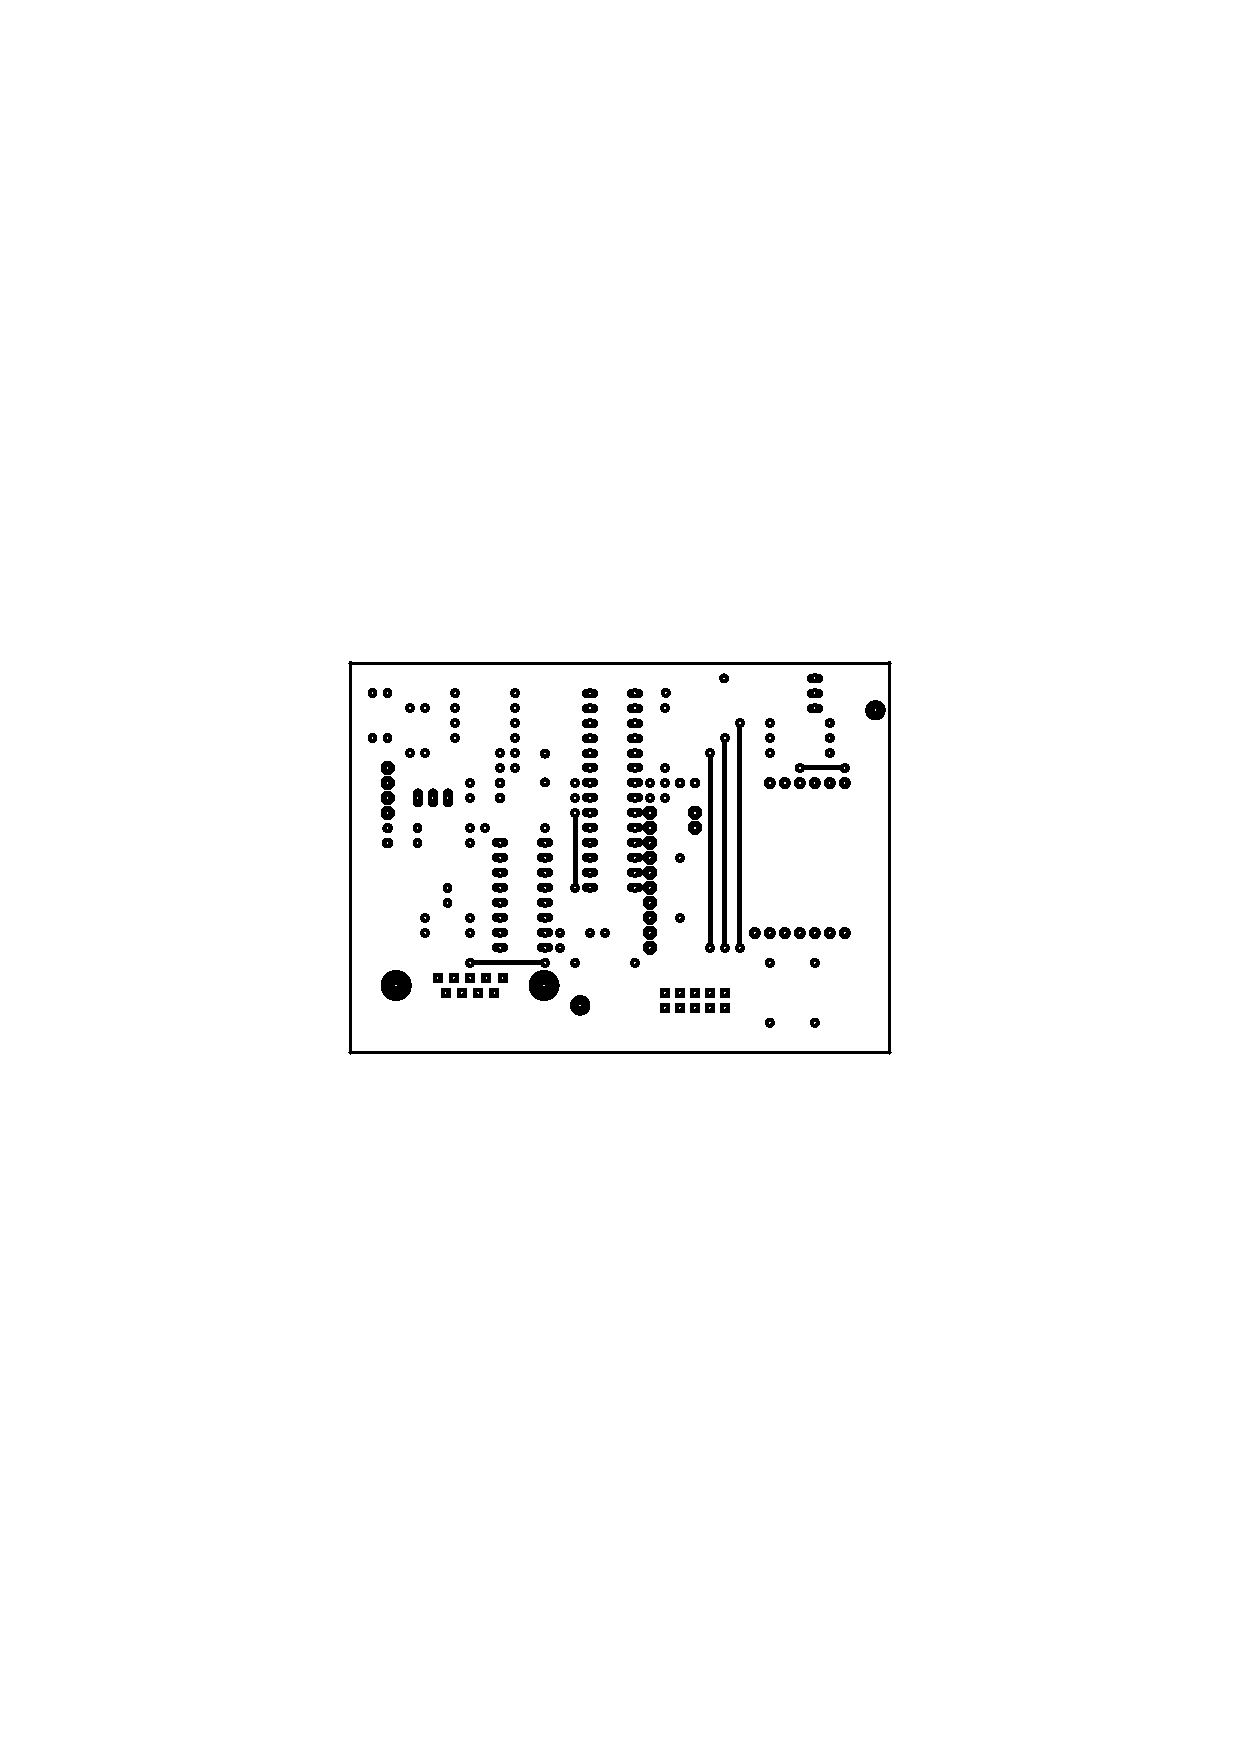
\includegraphics[scale=1]{Bilder/Transmittertop}\vspace{5mm}\\
				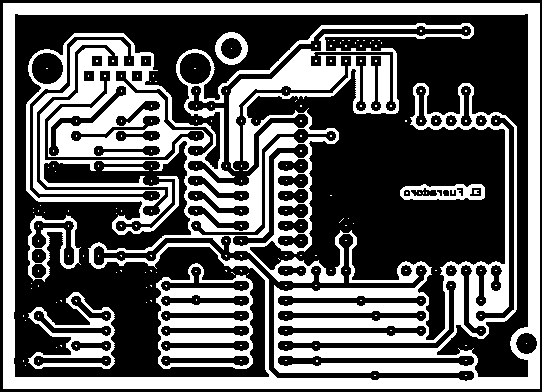
\includegraphics[scale=1]{Bilder/Transmitterbottom}
				\caption{Ober- und Unterseite des Transmitters für Toner-Transfer-Verfahren/Belichtung}
				\label{fig:transmitterprint}
			\end{figure}

			\begin{figure}
				\centering
				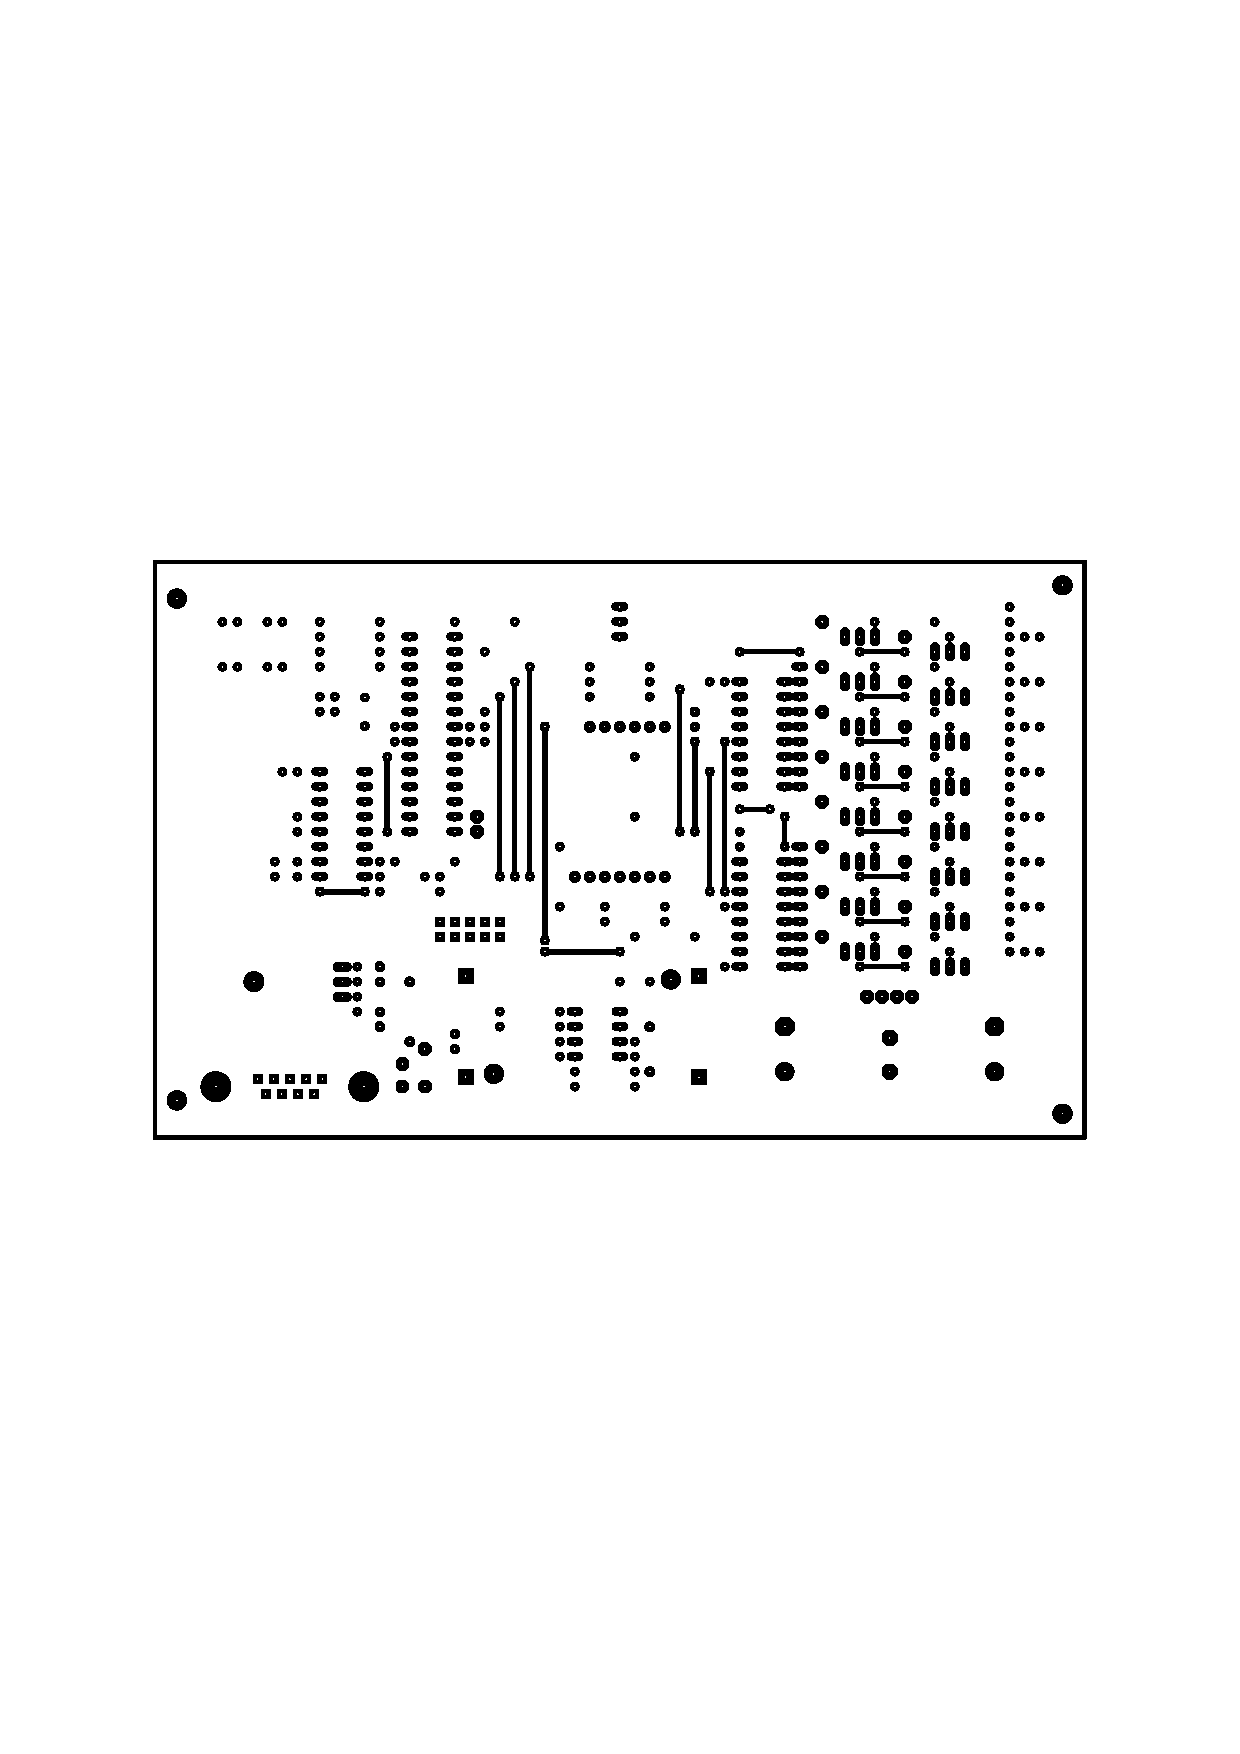
\includegraphics[scale=1]{Bilder/Zuendboxtop}\vspace{5mm}\\
				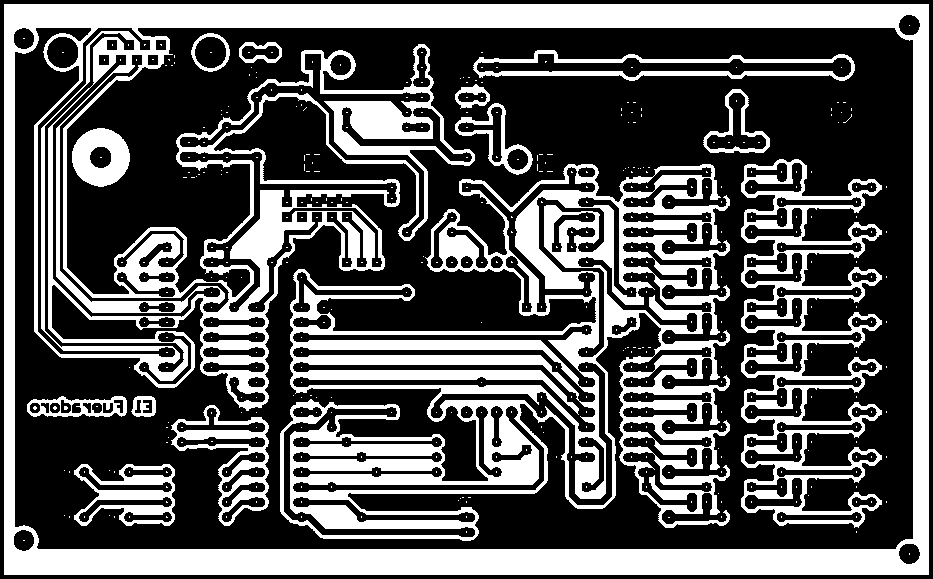
\includegraphics[scale=1]{Bilder/Zuendboxbottom}
				\caption{Ober- und Unterseite der Zündbox für Toner-Transfer-Verfahren/Belichtung}
				\label{fig:zuendboxprint}
			\end{figure}

			\begin{figure}
				\centering
				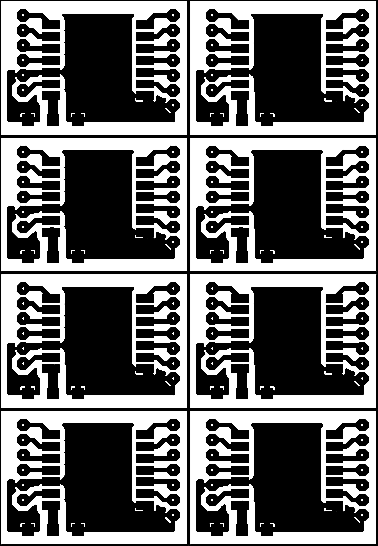
\includegraphics[scale=1]{Bilder/rfm-dil-70x100}
				\caption{Adapterplatine für Funkmodule (8 Stück) für Toner-Transfer-Verfahren/Belichtung}
				\label{fig:rfmprint}
			\end{figure}

			Die Layouts der zweiten Zündboxgeneration und der Raspberry-Pi-Aufsteckplatine sind aufgrund ihrer Komplexität nicht als Tonertransfer-Vorlagen verfügbar, hier kann auf einen der mittlerweile relativ günstigen PCB-Fertiger zurückgegriffen werden. Für Selbstfertigung kann man die Fertigungsdaten den jeweiligen Gerberdateien entnehmen.

		\chapter{Aufbau}

			\section{PC-Transmitter und Zündbox}

				Der Aufbau umfasst alle Schritte von der blanken Platine hin zum fertigen Gehäuse/Koffer. Hierfür sind verschiedene handwerkliche Tätigkeiten, vor allem das Elektroniklöten\footnote{Ein gutes~-- wenn auch englischsprachiges~-- Löt-Tutorial mit wichtigen Grundlagen gibt es \href{https://www.youtube.com/watch?v=I_NU2ruzyc4}{HIER}}, aber auch das Bohren, Schneiden, Kleben und evtl. Trennen mittels Trennscheibe und Feilen nötig.

				Im eigenen Interesse ist darauf zu achten, diese Arbeiten sorgfältig und unter Einhaltung der gängigen Sicherheitsregeln durchzuführen. \textbf{Beim Bohren und Trennen Schutzbrille tragen!} Beim Löten ist auf richtige Orientierung aktiver Bauteile (Dioden, Elektrolytkondensatoren, Temperatursensor, Integrierte Schaltungen) sowie Anschlusskabel zu achten, vor dem Einschalten soll die eigene Arbeit auch kritisch auf beim Löten entstandene Kurzschlüsse getestet werden\footnote{\href{http://www.youtube.com/watch?v=79dauuviLe4}{Hier klicken, um zu sehen, was ein kurzgeschlossener Blei-Gel-Akku mit Drähten/Leiterbahnen anstellt, sofern er nicht direkt explodiert!}}. Eine Laborspannungsquelle mit einstellbarer Strombegrenzung~-- oder ein Steckernetzteil mit maximal 2\,A Ausgangsstrom~-- zu Testzwecken tun hier gute Dienste, wobei auf die Einhaltung der zulässigen Betriebsspannungen (Transmitter 5-7\,V, Zündbox 8-15\,V) zu achten ist.

				\subsection{Kabel}

					Zur Verbindung der Platinen mit der Peripherie wird bei {\anlage} eine Vielzahl von Kabeln benötigt, die grob in drei Kategorien unterteilt werden können:
					\begin{enumerate}
						\item  Flachbandkabel bzw. Flachbandkabel-Adern zum Anschluss von LCD (außer Hintergrundbeleuchtung), LEDs und Schlüsselschalter
						\item Litze mit einer Querschnittsfläche von mindestens 0,5\,mm$^2$, d.\,h. einem Mindestdurchmesser von 0,8\,mm, zum Anschluss von LCD-Hintergrundbeleuchtung, Netzschalter und
								Zündklemmen
						\item 50\,$\Omega$-Koaxialkabel als Antennenkabel
					\end{enumerate}

					Die Koaxialkabel werden in diesem Abschnitt nicht behandelt, da dafür oft Spezialwerkzeug notwendig ist und davon ausgegangen wird, dass diese Kabel bereits fertig konfektioniert erworben werden. Für die Konfektionierung der anderen Kabel gilt, dass diese so kurz wie möglich aber gleichzeitig auch so lang wie nötig sein sollten, um das Verlöten/Verkleben annehmbar zu gestalten und das Gehäuse später noch einmal öffnen zu können, ohne gleich alles abzureißen.

					\begin{table}
						\centering
						\begin{tabularx}{\textwidth}{cccccX}
							\hline\hline
							Device (T/Z) & Art       & Adern & Länge  & Anzahl & Verwendungszweck              \\
							Z            & Litze     & ~--   & 210 mm & 4      & Rote Klemmen (spaltenweise)   \\
							Z            & Litze     & ~--   & 210 mm & 16     & Schwarze Klemmen              \\
							Z            & Litze     & ~--   & 200 mm & 2      & Netzschalter                  \\
							Z            & Litze     & ~--   & 250 mm & 4      & Batterie (2x rot, 2x schwarz) \\
							Z            & Flachband & 2     & 200 mm & 16     & Kanal-LEDs                    \\
							Z            & Flachband & 2     & 200 mm & 4      & Status-LEDs                   \\
							Z            & Flachband & 2     & 200 mm & 1      & Schlüsselschalter             \\ \hline
							T            & Litze     & ~--   & 100 mm & 2      & LCD-Hintergrundbeleuchtung    \\
							T            & Flachband & 2     & 100 mm & 4      & Status-LEDs                   \\
							T            & Flachband & 10    & 100 mm & 1      & LCD                           \\ \hline\hline
						\end{tabularx}
						\caption{Übersicht über benötigte Kabelverbindungen}
						\label{tab:kabel}
					\end{table}

					In Tabelle~\ref{tab:kabel} sind die benötigten Abschnitte aufgelistet. Alle Kabel sollten am einen Ende jeweils auf einer Länge von 4\,mm zum Festlöten an der Platine, am anderen auf einer Länge von 6\,mm abisoliert und verzinnt werden. Zur Vereinfachung der Arbeit ist es ratsam, die Adern des Flachbandkabels erst danach zu trennen, so dass nicht jeder \enquote{Zweierverbund} einzeln abisoliert und verzinnt werden muss.

					Es dient der Übersichtlichkeit und dem späteren Verständnis ungemein, wenn man verschiedene Kabelfarben verwendet und sich dabei an gängige Konventionen hält (Akkuspannung rot, Masse schwarz).

				\subsection{Platinen}

					Ausgangspunkt der Bestückung ist die geätzte und gebohrte Platine mit allen Leiterbahnen auf der Ober- und Unterseite. Für selbst gefertigte, einseitig geätzte Platinen, bei denen die Leitungen auf der Oberseite als Drahtbrücken ausgeführt sind, sind diese in Abbildung~\ref{fig:platinen} dargestellt.

					\begin{figure}[t]
						\centering
						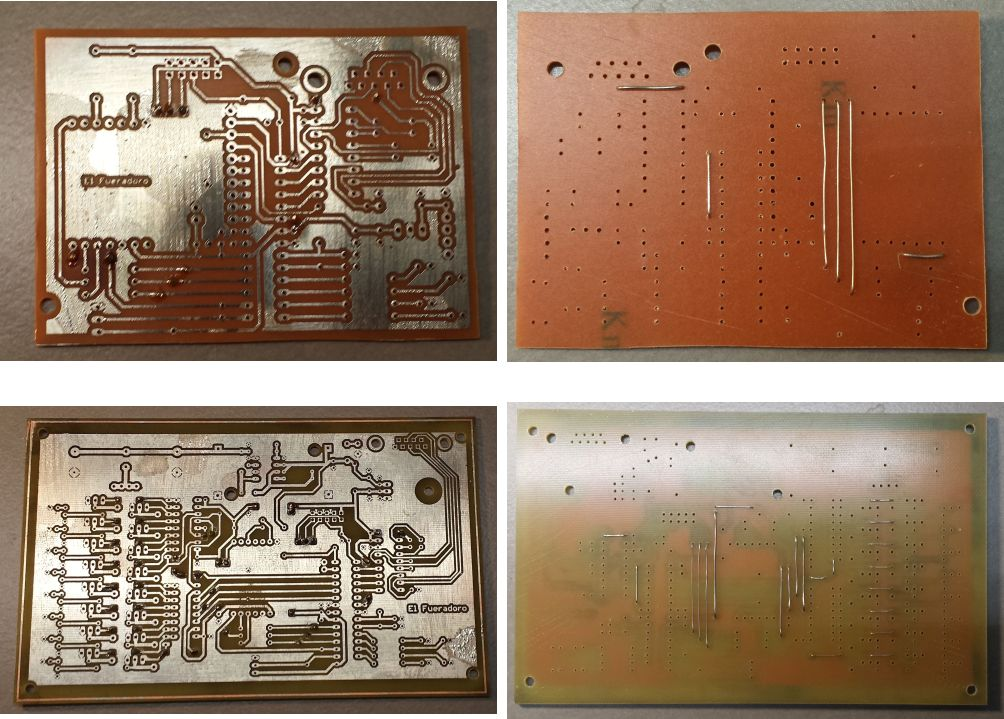
\includegraphics[width=\textwidth]{bilder/platinen}
						\caption{Platinen für Transmitter (oben) und Zündbox (unten)}
						\label{fig:platinen}
					\end{figure}

					Anschließend sollten die Bauteile in folgender Reihenfolge eingelötet werden:
					\begin{description}
						\item[Widerstände] mit Ausnahme von R\_Z
						\item[Dioden] mit korrekter Polung
						\item[Keramikkondensatoren]
						\item[Quarz]
						\item[Buchsenleisten] für Funkmoduladapter
						\item[Elektrolytkondensatoren] Polung beachten und C14 beim Transmitter waagrecht legen!
						\item[Leistungswiderstand] R\_Z
						\item[Temperatursensor] mit korrekter Orientierung
						\item[Integrierte Schaltungen] mit korrekter Orientierung
								\begin{center}
									Der Stand bis zu diesem Punkt ist in Abbildung~\ref{fig:platinenzwischenschritt} dargestellt.
								\end{center}
						\item[Anschluss-Kabel] für Klemmen (Zündbox) bzw. LCD (Transmitter)
						\item[Schalterkabel] für Netz- und Schlüsselschalter
						\item[LED-Kabel] für Status-LEDs und Kanal-LEDs. Um den Überblick zu behalten sollte dabei jeweils das Kabel für den GND-Anschluss vor dem Einlöten markiert werden
						\item[MOSFETs] mit korrekter Orientierung (Metallplatte sitzt auf der Seite der großen Elkos)
						\item[Batterie- bzw. USB-Versorgungs-Kabel] Falls bei der Zündbox fertig konfektionierte Kabel mit Anschluss verwendet werden, vor dem Löten die Seitenwand auf der Schalterseite durchbohren und beide Kabel durchfädeln. Beim Trasmitter wird das Kabel zwischen zwei miteinander verschraubten Teilen verlegt.
					\end{description}

					\begin{figure}
						\centering
						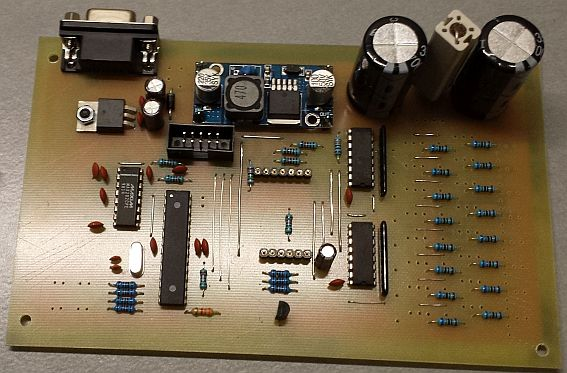
\includegraphics[width=\textwidth]{bilder/platinenzwischenschritt}
						\caption{Zündboxplatine (1. Generation) vor dem Einlöten der Kabel und MOSFETs}
						\label{fig:platinenzwischenschritt}
					\end{figure}

			\section{Raspberry-Pi-Aufsteckplatine}

				Das Einlöten der Bauteile erfolgt in bewährter Reihenfolge:
				\begin{description}
					\item[Widerstände]
					\item[Keramikkondensatoren]
					\item[Einreihige Buchsenleisten] für Funkmoduladapter
					\item[Schraubklemmen]
					\item[Elektrolytkondensatoren] Polung beachten!
					\item[Integrierte Schaltungen] mit korrekter Orientierung
					\item[Zweireihige Buchsenleiste] ACHTUNG: Buchsenleiste befindet sich auf der Unterseite der Platine, Lötseite ist also hier ausnahmsweise die Oberseite
					\item[Verbindungskabel] zwischen Spannungsmesspunkt und Klemmeneingang
				\end{description}

				Die fertig bestückte Platine ist in Abbildung~\ref{fig:raspiextension} gezeigt.

				\begin{figure}
					\centering
					%\includegraphics[width=\textwidth]{bilder/raspiextension}
					{\LARGE Bild folgt!}
					\caption{Raspberry-Pi-Erweiterungsplatine}
					\label{fig:raspiextension}
				\end{figure}

			\section{Funkmodul-Adapter}

				Nachdem die Platinen nun fertig bestückt sind, folgen die Schritte für die Fertigstellung des Funkmodul-Adapters:
				\begin{description}
					\item[Funkmodul] mit allen 14 Anschlüssen (Orientierung beachten) auf der Adapterplatine festlöten. Dabei beachten, dass auf die SMD-Pads auf beiden Seiten etwa gleich weit unter den Anschlüssen hervorstehen und das Modul nicht nach oben oder unten verschoben ist. Am besten mit dem mittleren Pin einer Seite beginnen und das Modul beim Löten korrekt positionieren, dann alle anderen 13 Anschlüsse löten.
					\item[SMA-Buchse] anlöten, so dass sie direkt an der Platine anliegt. Falls Anschlüsse zu lang sind und am Modul anstoßen, vorsichtig mit Trennscheibe (Außenleiter) oder Seitenschneider (Innenleiter) kürzen.
					\item[Stiftleiste] in einen 6-poligen und einen 7-poligen Abschnitt teilen und anlöten.
				\end{description}

				\begin{figure}
					\centering
					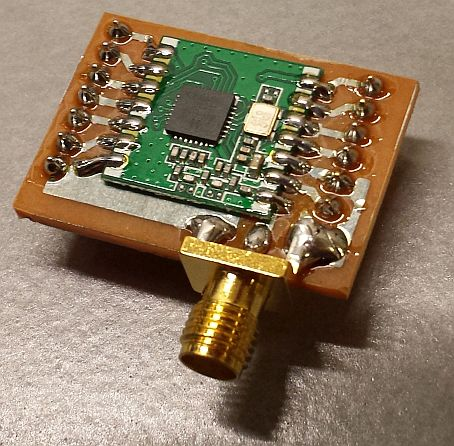
\includegraphics[width=.5\textwidth]{bilder/funkmoduladapter}
					\caption{Fertig aufgebauter Funkmoduladapter}
					\label{fig:funkmoduladapter}
				\end{figure}

				Der fertige Adapter ist in Abbildung~\ref{fig:funkmoduladapter} gezeigt.

			\section{Peripherie}

				\subsection{Transmitter}
					Als Gehäuse für den Transmitter wird das schwarze Kunststoffgehäuse GEH KS 50 aus dem Sortiment von Reichelt verwendet. Es besteht aus zwei miteinander zu verschraubenden Teilen, wobei der dünne Teil, auf dem später die Platine befestigt wird, als Rückwand dient. Dementsprechend sind die Bezeichnungen in der folgenden Beschreibung zu verstehen.

					\begin{figure}
						\centering
						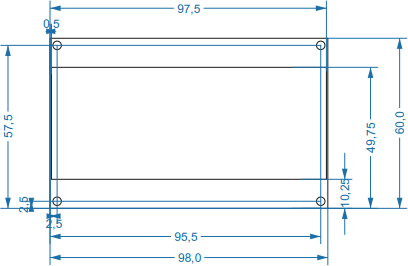
\includegraphics[]{bilder/lcddimensions}
						\caption{Abmessungen (in mm) des LCD}
						\label{fig:lcddimensions}
					\end{figure}

					Die Vorderseite des Gehäuses muss zunächst mit einem Ausschnitt von $\SI{97}{\milli\metre}\,\times\,\SI{39,5}{\milli\metre}$ und vier $\SI{3}{\milli\metre}$-Bohrungen für die Anbringung des LCD versehen werden. Die Abstände zueinander sind in Abbildung~\ref{fig:lcddimensions} verdeutlicht. Wer nicht auf seine Messkünste vertrauen möchte oder ein LCD mit abweichenden Abmessungen besitzt, sollte zunächst einen passenden Ausschnitt für den Bildschirm mittig in der Fläche anbringen, anschließend können das LCD aufgelegt und die vier Bohrlöcher markiert und gebohrt werden.

					Bevor man das LCD einschraubt, muss noch eine Aussparung für den Sub-D-Anschluss, ein Loch für den Antennenanschluss ($\SI{6,5}{\milli\metre}$), vier Löcher für die Status-LEDs ($\SI{5}{\milli\metre}$)und eine Kerbe für die Versorgungskabeldurchführung in die Wand, welche später als Oberseite des Gehäuses dient, eingebracht werden.

					Hierfür sollte man zunächst die fertig bestückte Platine mittels zweier Schrauben in ihrer finalen Position festschrauben und das Oberteil so anlegen, dass die Position der Aussparung für die Sub-D-Buchse angezeichnet werden kann. Die Abmessung der Aussparung sollte $\SI{31}{\milli\metre}\,\times\,\SI{12,5}{\milli\metre}$ betragen. Die Positionen der restlichen Löcher sind aufgrund der Kabelverbindung mit der Platine unkritisch, die ungefähre Lage kann Abbildung~\ref{fig:transmitter} auf Seite \pageref{fig:transmitter} entnommen werden. Das Versorgungskabel mit USB-Stecker wird zwecks Zugentlastung zwischen den beiden zu verschraubenden Teilen eingeklemmt, die Kerbe sollte daher nicht allzu groß ausgeführt werden. Die Bohrarbeiten am Transmitter sind damit erledigt!

					Nun müssen noch die elektrischen Verbindungen zwischen Platine und Peripherie hergestellt und die Peripherieteile anschließend befestigt werden~-- zuerst die vier Status-LEDs:

					\begin{enumerate}
						\label{enum:leds}
						\item Die Verbindung der Adern des Flachbandkabels auf einer Länge von etwa $\SI{35}{\milli\metre}$ auftrennen
						\item Auf jede Ader einen dünnen Schrumpfschlauch der Länge $\SI{15}{\milli\metre}$ stecken (noch nicht erhitzen!)
						\item Das kürzere Anschlussbein der LED (Kathode) mit dem Seitenschneider auf eine Länge von $\SI{8}{\milli\metre}$ trimmen und die mit GND verbundene Ader anlöten
						\item Das längere Anschlussbein der LED (Anode) mit dem Seitenschneider auf eine Länge von $\SI{8}{\milli\metre}$ trimmen und die andere Ader anlöten
						\item Schrumpfschläuche bis ans LED-Gehäuse vorschieben und per Heißluft schrumpfen
					\end{enumerate}

					Anschließend das Flachbandkabel für das LCD vorbereiten, d.\,h. abisolieren, verzinnen und Verbindungen soweit lösen, dass alle Anschlüsse bequem erreicht werden können. Da das LCD im 4-Bit-Modus betrieben wird, werden nur die Pins 1-6 sowie 11-16 angeschlossen, 7-10 bleiben offen. Bei Anschluss der Pins 15 und 16 darauf achten, Anode und Kathode nicht zu vertauschen; die Belegung ist in der Regel so, dass die Anode an Pin 15 herausgeführt ist, kann aber von LCD zu LCD variieren. Der Lötkolben kann danach ausgeschaltet werden, jetzt geht es an die Befestigung.

					Zunächst wird das LCD am Gehäuse festgeschraubt, wobei darauf zu achten ist, dass die Oberseite auch in die Richtung von Antennen- und Sub-D-Anschluss zeigt. Anschließend die LEDs um den Gehäusering mit Sekunden- oder Heißkleber bestreichen und danach für einige Sekunden fest ins dafür vorgesehene Loch pressen. Nun die SMA-Buchse fest am Gehäuse anschrauben und das andere Kabelende mit der Buchse am Funkmodul-Adapter verbinden.

					Unter möglichst geringer Torsion sollte dann der Funkmoduladapter in die Buchsenleisten auf der Platine gesteckt werden.

					Nun muss man noch die Antenne anschrauben. Wenn der Bootloader sich bereits auf dem Controller befindet, kann man das Gehäuse zuschrauben. Ansonsten den Transmitter mit Energie versorgen und den Bootloader wie in Abschnitt~\ref{ch:bootloader} beschrieben flashen. Jetzt ist der Transmitter fertig aufgebaut und kann zugeschraubt werden! Die Firmware kann wie in Abschnitt~\ref{ch:firmwareupdate} beschrieben über die serielle Schnittstelle aufgespielt werden, wobei beim ersten Mal noch die Angabe des Dateinamens nötig ist.

				\subsection{Zündbox}
					Abbildung~\ref{fig:zuendboxbohren} zeigt die Bohrschablone für die Oberseite des Kunststoffgehäuses der Zündbox (Kunststoffgehäuse 021-002-084 von Pollin). Diese kann dazu verwendet werden, eine Schablone aus Sperrholz oder Metall anzufertigen, welche später auf die Boxenoberseite gelegt wird, um die nötigen Bohrungen vorzunehmen. Die Oberseite des Gehäuses ist dabei der Teil ohne sichtbare Schraublöcher.

					\begin{figure}
						\centering
						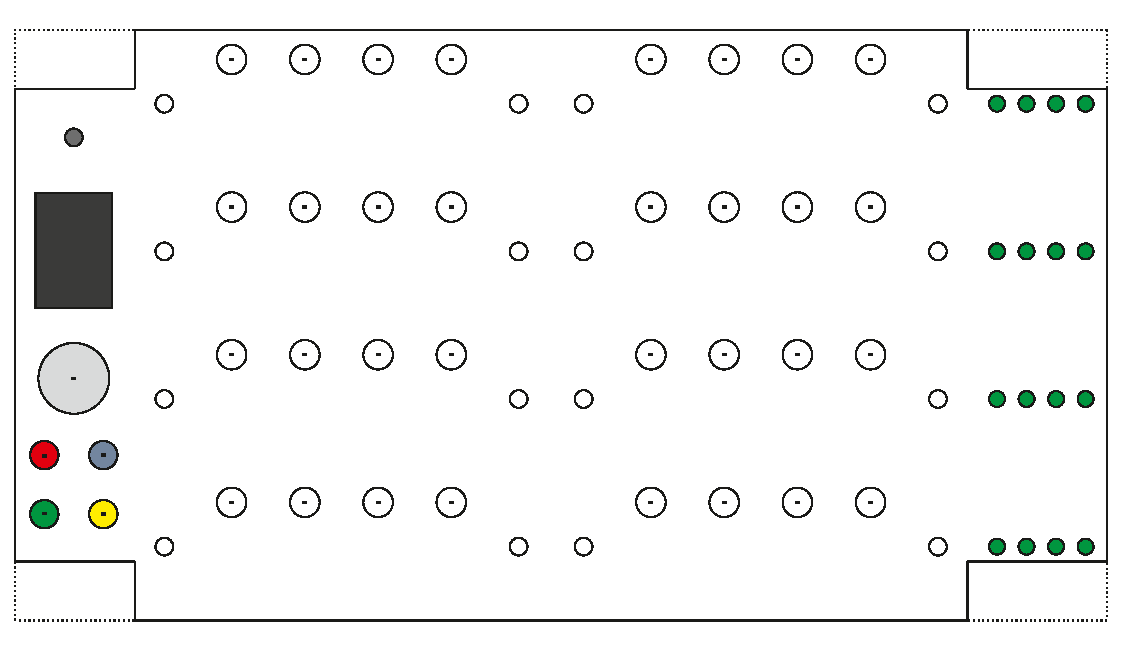
\includegraphics[angle=90,scale=1]{Bilder/Zuendboxbohrschablone}
						\caption{Bohrschablone für Zündboxoberseite}
						\label{fig:zuendboxbohren}
					\end{figure}

					Es ist beim Bohren der Box auf die richtige Orientierung der Schablone zu achten, da die Befestigungsbohrungen für die Platine nicht symmetrisch sind (Schrauben auf der linken Seite, wo sich die serielle Schnittstelle befindet, sind enger zusammen als die auf der rechten Seite mit den MOSFETs und Kanal-LEDs) und die Gehäuseteile durch ein Nut-Feder-System nur in einer Kombination aufeinander gesteckt werden können. Man beachte hierzu Abbildung~\ref{fig:zuendboxdeckel}.

					Damit die Löcher nicht mit Schraubenhalterungen in den Ecken interferieren, sollte zunächst im Gehäuseinneren der passende Ort für die Kanal-LEDs von Kanal 4 und 16 (äußerste grüne LEDs in der obersten und untersten Reihe, Abstand $\SI{75}{\milli\metre}$) gesucht, die beiden Löcher mit einem $\SI{3}{\milli\metre}$-Bohrer gebohrt und die Schablone auf der Oberseite in diesen beiden Bohrungen befestigt werden.

					Die Bohrlöcher für die 16 Kanal-LEDs sollten mit einem 3-mm-Bohrer, die der vier Status-LEDs mit einem $\SI{5}{\milli\metre}$-Bohrer ausgeführt werden. Die LEDs werden später (nach dem Verkabeln und Festlöten des Kabels auf der Platine) seitlich mit Heißkleber bestrichen von unten bis zum Anschlag in diese Löcher eingeschoben.

					Da die Lautsprecherklemmen mit M3-Gewindeschrauben befestigt werden, wäre der ideale Bohrdurchmesser für die 16 Schraubenlöcher $\SI{3,2}{\milli\metre}$. Sollte dieser Durchmesser nicht vorhanden sein, kann aber auch mit $\SI{3,5}{\milli\metre}$ oder $\SI{3}{\milli\metre}$ gearbeitet werden. Für die Lötfahnen der Klemmen ist eine rechteckige Aussparung von $\SI{4,5}{\milli\metre}\,\times\,\SI{2}{\milli\metre}$ nötig, als schnelle Lösung kann auch jeweils ein $\SI{5}{\milli\metre}$-Loch durch den Mittelpunkt (Diagonalenschnittpunkt) dieser Flächen gebohrt werden.

					Die rechteckige Aussparung für den Netzschalter sollte die Größe $\SI{19}{\milli\metre}\,\times\,\SI{13}{\milli\metre}$ besitzen, der Schlüsselschalter hat einen Einbaudurchmesser von $\SI{12}{\milli\metre}$ und der Durchsteckplatz für die SMA-Buchse sollte mit $\SI{6,5}{\milli\metre}$ vorgebohrt werden. Im nächsten Schritt werden Schlüsselschalter, Klemmen und Netzschalter am Gehäuse verschraubt bzw. eingeklickt. Die Innenansicht des Zündboxdeckels (noch ohne SMA-Anschluss) ist in Abbildung~\ref{fig:zuendboxdeckel} dargestellt. Hierbei ist auch zu erkennen, wo sich die Nut (unten, bei den Status-LEDs) und wo die Feder (oben) beim Deckel befinden muss. Dementsprechend muss es bei der Unterseite andersherum sein.

					\begin{figure}
						\centering
						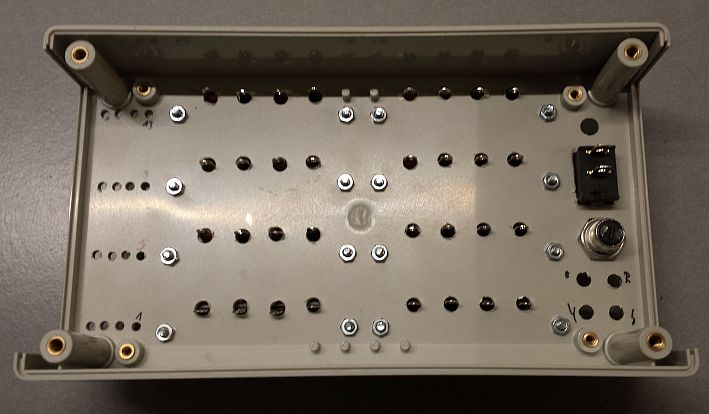
\includegraphics[width=\textwidth]{bilder/zuendboxdeckel}
						\caption{Innenansicht des Zündboxdeckels}
						\label{fig:zuendboxdeckel}
					\end{figure}

					In die linke Einschub-Seitenwand muss, sofern noch nicht im Rahmen des Lötens geschehen, ein Loch für die Durchführung der Batteriekabel mit einer Größe je nach Kabeldurchmesser.

					Um die Position der Sub-D-Buchse in der Wand des Unterteils, welche in der Nut endet, zu finnden, muss die Platine möglichst identisch zu ihrer späteren Position ins Gehäuse eingelegt werden, die Aussparung beträgt wie beim Transmitter $\SI{31}{\milli\metre}\,\times\,\SI{12,5}{\milli\metre}$. Wenn die Aussparung fertig ist, kann die Platine in ihre endgültige Position gebracht und mit vier Schrauben befestigt werden. Die linke Seitenwand bleibt noch ausgesteckt. Jetzt ist wieder der Lötkolben dran!

					Zunächst vier Drahtstücke á $\SI{80}{\milli\metre}$ abschneiden und durch die übereinander liegenden Lötfahnen der roten Klemmen ziehen und mit den Lötfahnen verlöten.

					Die Kanal- und Status-LEDs wie auf Seite \pageref{enum:leds} beschrieben mit den zugehörigen Flachbandkabeln verbinden, anschließend den Schlüssel- und den Netzschalter mit den zugehörigen Anschlusskabeln.

					Bei den Schritten in den folgenden Absätzen ist Sorgfalt geboten, da die Kanäle und LEDs richtig zugeordnet werden müssen, um später mit dem entsprechenden Befehl auch den richtigen Kanal zu zünden!

					Zunächst müssen die 16 Kabel mit den zugehörigen schwarzen Klemmen verbunden werden, was anhand des Layouts in Abbildung~\ref{fig:zuendboxlayout} auf Seite \pageref{fig:zuendboxlayout} erklärt werden soll. Kanal 1 wird vom Transistor Q2 gesteuert, Kanal 2 von Q3, Kanal 3 von Q4 und allgemein Kanal x-1 von Qx. Entsprechend ist das Kabel, welches an derjenigen Lötstelle angelötet ist, die durch die dicke blaue Linie unmittelbar mit dem mittleren Pin (Drain) von Q2 verbunden ist, an der Lötfahne der schwarzen Klemme ganz unten links~-- bezogen auf Abbildung~\ref{fig:zuendbox}~-- anzubringen. Das Kabel an der Drain von Q3 (Zick-Zack-Anordnung der Transistoren beachten!) wird mit der schwarzen Klemme daneben verbunden, das an Q4 mit der dritten und das an Q5 schließlich mit der letzten Klemme in der Reihe, die unmittelbar neben der Viererreihe für die Kanal-LEDs liegt. Man sollte sich nicht dadurch verwirren lassen, dass aufgrund des umgedrehten Deckels alles seitenverkehrt ist, man die Klemmen also beim Löten von rechts nach links belegt. Analog zum bisherigen Vorgehen verfährt man in der Reihe darüber und den beiden anderen Reihen.

					Nun werden mit Heiß- oder Sekundenkleber die Kanal-LEDs in die richtige Position gesteckt.

					Für Kanal n ist dabei immer auch LEDn zuständig, für Kanal 1 also LED1, die über R21 mit der Drain von Q2 verbunden ist, für Kanal 2 LED2, usw. Sinnvollerweise ist LED1 in das Loch zu kleben, welches in der untersten Reihe direkt neben den Klemmen liegt, LED8 dementsprechend in der zweituntersten Reihe ganz außen usw.

					Danach werden die vier Kabel am Leistungswiderstand jeweils mit einem der gespannten Drähte an den roten Klemmen verbunden. Hierbei spielt die Zuordnung (welches Kabel an welchen Draht?) keine Rolle. Damit sind sämtliche Kabel im inneren der Box nun verlötet und die Arbeit nähert sich langsam dem Ende!

					Nun die SMA-Buchse fest am Gehäuse anschrauben, die Antenne vorerst dort befestigen und das andere Kabelende mit der Buchse am RFM-Adapter verbinden. Unter möglichst geringer Torsion sollte dann der RFM-Adapter mit dem aufgelöteten Funkmodul in die Buchsenleisten auf der Platine gesteckt werden.

					Wenn der Bootloader bereits auf den Controller geflasht wurde, kann man jetzt die beiden Seitenwände einstecken und die Box zuschrauben (wenn man sich sicher ist, dass sie funktioniert\dots). Ansonsten muss die Box noch offen bleiben.

					Den männlichen Teil des Steckerpaars mit den aus der Box kommenden Batteriekabeln verlöten (Schrumpfschlauch nicht vergessen!), den weiblichen über zwei Kabel an der Batterie, wobei jeweils auf die korrekte Polung zu achten ist\footnote{Bei Deans-T-Steckern wird der obere Balken des T mit + verbunden, bei Tamiya-Steckern das eckige Profil}.

					Für die erste Inbetriebnahme sollte, wie zu Beginn des Kapitels empfohlen, idealerweise eine Laborspannungsquelle, ein kurzsschlussfestes Steckernetzteil oder aber eine träge 3 A-Sicherung in der Zuleitung verwendet werden. Nun die Box über den Netzschalter einschalten und, falls noch nicht geschehen, den Bootloader via ISP flashen. Nun kann die Box zugeschraubt und die
					Firmware eingespielt werden.

				\subsection{Koffer}

					Als Aufbewahrungsort für die Zündboxen tut ein robuster Aluminiumkoffer wertvolle Dienste, um die Zündboxen vor Wettereinflüssen und Feuerwerks\-nieder\-schlag zu schützen. Als gutes Pendant zum Plastikgehäuse bietet sich der in der Materialliste in Tabelle~\ref{tab:zuendbox2bom} aufgeführte Alu-Koffer 545 von Bilora an, der gerade ausreichend Platz für eine Zündbox und den zugehörigen Blei-Gel-Akku für die Stromversorgung bietet.

					\subsubsection{Schaumstoffeinlage}

						Der Koffer besitzt eine gewürfelte Schaumstoffeinlage mit einem $18\,\times\,14$-Raster, die gemäß Abbildung~\ref{fig:foamcut} entsprechend angepasst werden kann, um auch beim Transport einen festen Stand von Zündbox und Akku im Koffer zu ermöglichen.

						\begin{figure}
							\centering
							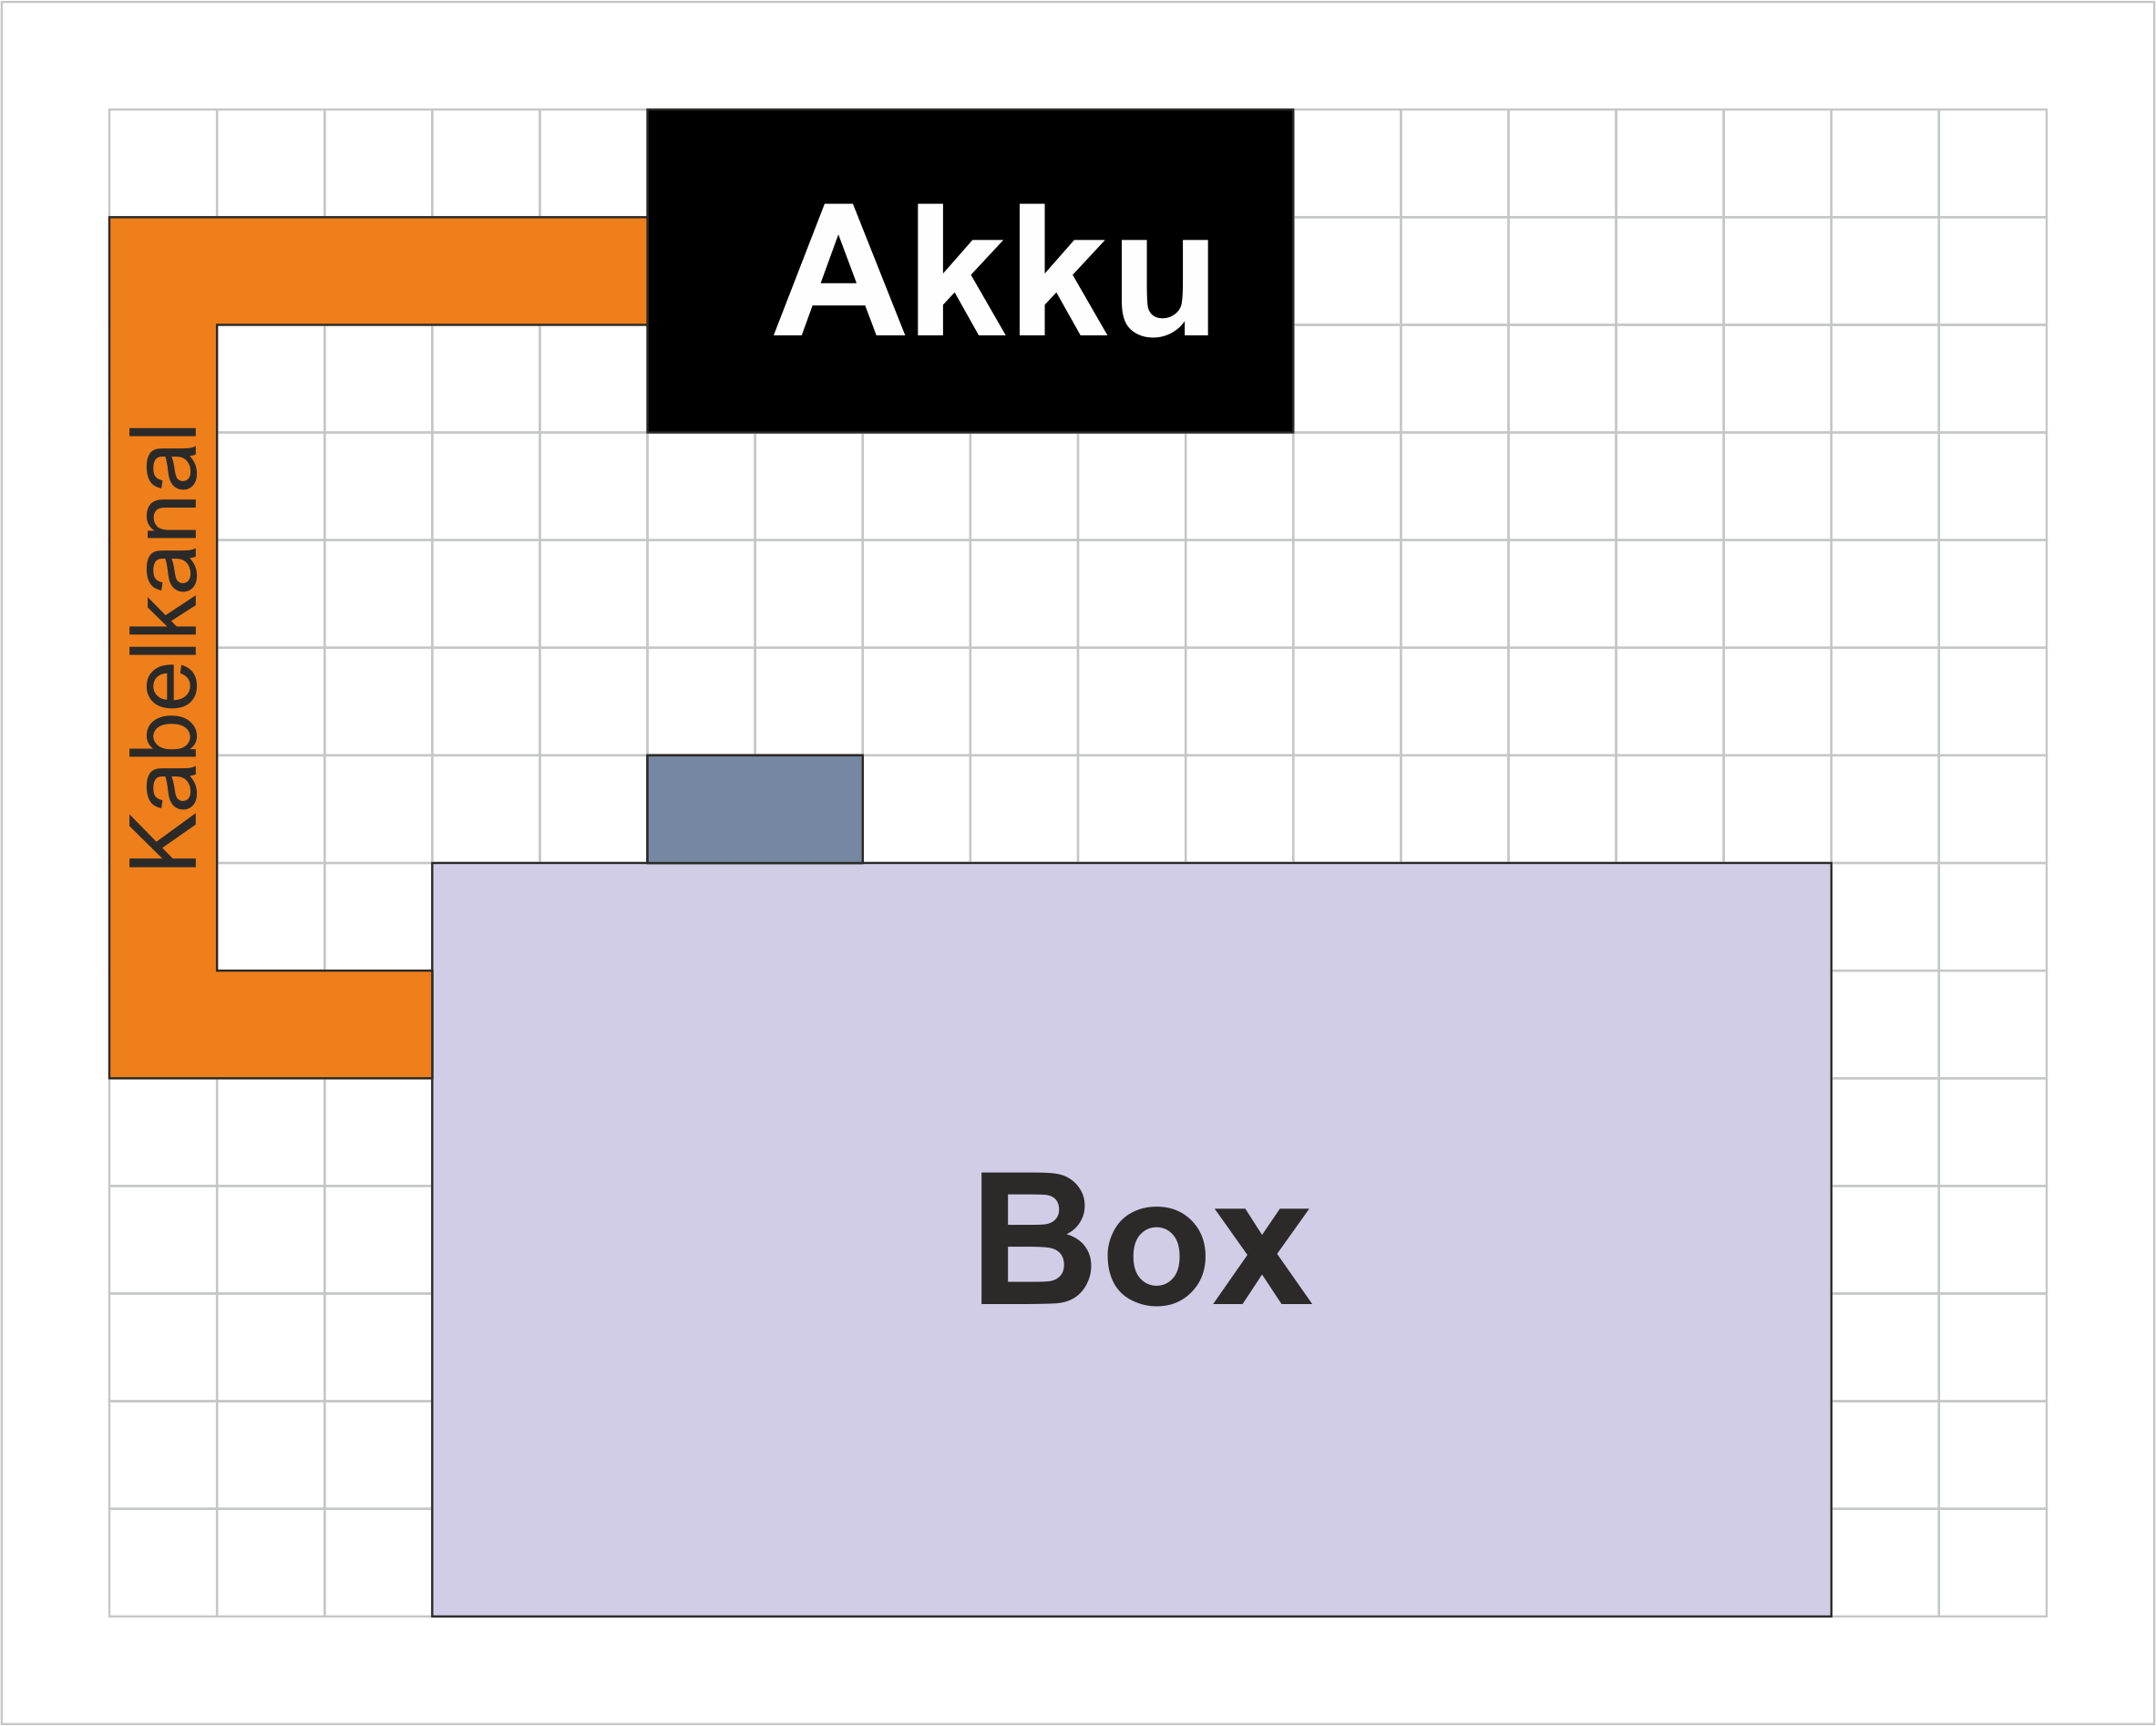
\includegraphics[width=.7\textwidth]{Bilder/foamcut.png}
							\caption{Ausschnitt aus der Schaumstoffeinlage für Zündbox und Akku}
							\label{fig:foamcut}
						\end{figure}

						Hierfür müssen für die Box $13\,\times\,7$ sowie für den Akku $6\,\times\,3$ Würfel händisch oder mit Hilfe eines Teppichmessers an den gezeigten Stellen gelöst werden. Zudem empfiehlt es sich noch, zwei Würfel an der seriellen Schnittstelle für ein leichteres Herausnehmen der Box und den eingezeichneten Kabelkanal herauszutrennen. Um ein Herauslösen weiterer Würfel zu verhindern, kann mittels Sekunden- oder Heißkleber in den Kreuzungen der vorgestanzten Linien eine festere Naht hergestellt werden.

					\subsubsection{Antennenhalterung}

						Etwas Arbeit ist nötig, um die Antenne in eine geeignete Position zu bringen, um bei geschlossenem Koffer die Zündkommandos noch sicher und zuverlässig empfangen zu können. Wenn die Antenne nicht außerhalb des Gehäuses angebracht ist, können ankommende Signale nicht bzw. nur äußerst stark gedämpft hinein- und abgehende so gut wie nicht hinausgelangen, weil der Alukoffer als Faradayscher Käfig wirkt.

						\begin{figure}
							\centering
							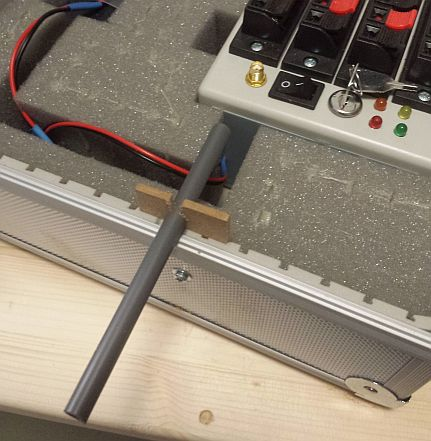
\includegraphics[width=.75\textwidth]{Bilder/koffer-adapter-montiert}
							\caption{Adapter am Koffer montiert}
							\label{fig:koffer-adapter-montiert}
						\end{figure}

						Um die Antenne vom SMA-Anschluss an der Zündbox nach außen zu führen, wird ein zweiteiliger Adapter, der in Abbildung~\ref{fig:koffer-adapter-montiert} am Koffer montiert gezeigt ist, verwendet. So wird einerseits das Kabel geschützt, andererseits die Kabelführung stabilisiert. Die Halterung besteht aus zwei ineinander gesteckten Teilen:
						\begin{itemize}
							\item MDF-Platte: $\SI{85}{\milli\metre} \times \SI{35}{\milli\metre} \times \SI{3}{\milli\metre}$
							\item PVC-Rohr, basierend auf einer Gardena-Micro-Drip-Verlängerung: $\oslash\SI{7,5}{\milli\metre} \times \SI{115}{\milli\metre}$
						\end{itemize}

						In die MDF-Platte wird $\SI{10}{\milli\metre}$ vom oberen Rand entfernt mehr oder weniger mittig ein $\SI{5}{\milli\metre}$-Loch gebohrt und ein Kanal senkrecht nach oben zum Rand eingebracht. Beim PVC-Rohr bringt man $\SI{7}{\centi\metre}$ vom Rand entfernt auf einer Länge von $\SI{3}{\milli\metre}$ zwei Einschnitte ein, um das Rohr an dieser Stelle auf die Breite des Kanals zu bringen. Die beiden Einzelteile sind in Abbildung~\ref{fig:koffer-adapter-einzeln}, der zusammengesteckte Adapter in Abbildung~\ref{fig:koffer-adapter-zusammen} abgebildet. Der Adapter wird vor dem Montieren der MDF-Platte am Koffer so ausgerichtet, dass die Rohröffnung genau auf die SMA-Buchse an der Zündbox zeigt.

						\begin{figure}
							\begin{subfigure}[t]{0.5\textwidth}
								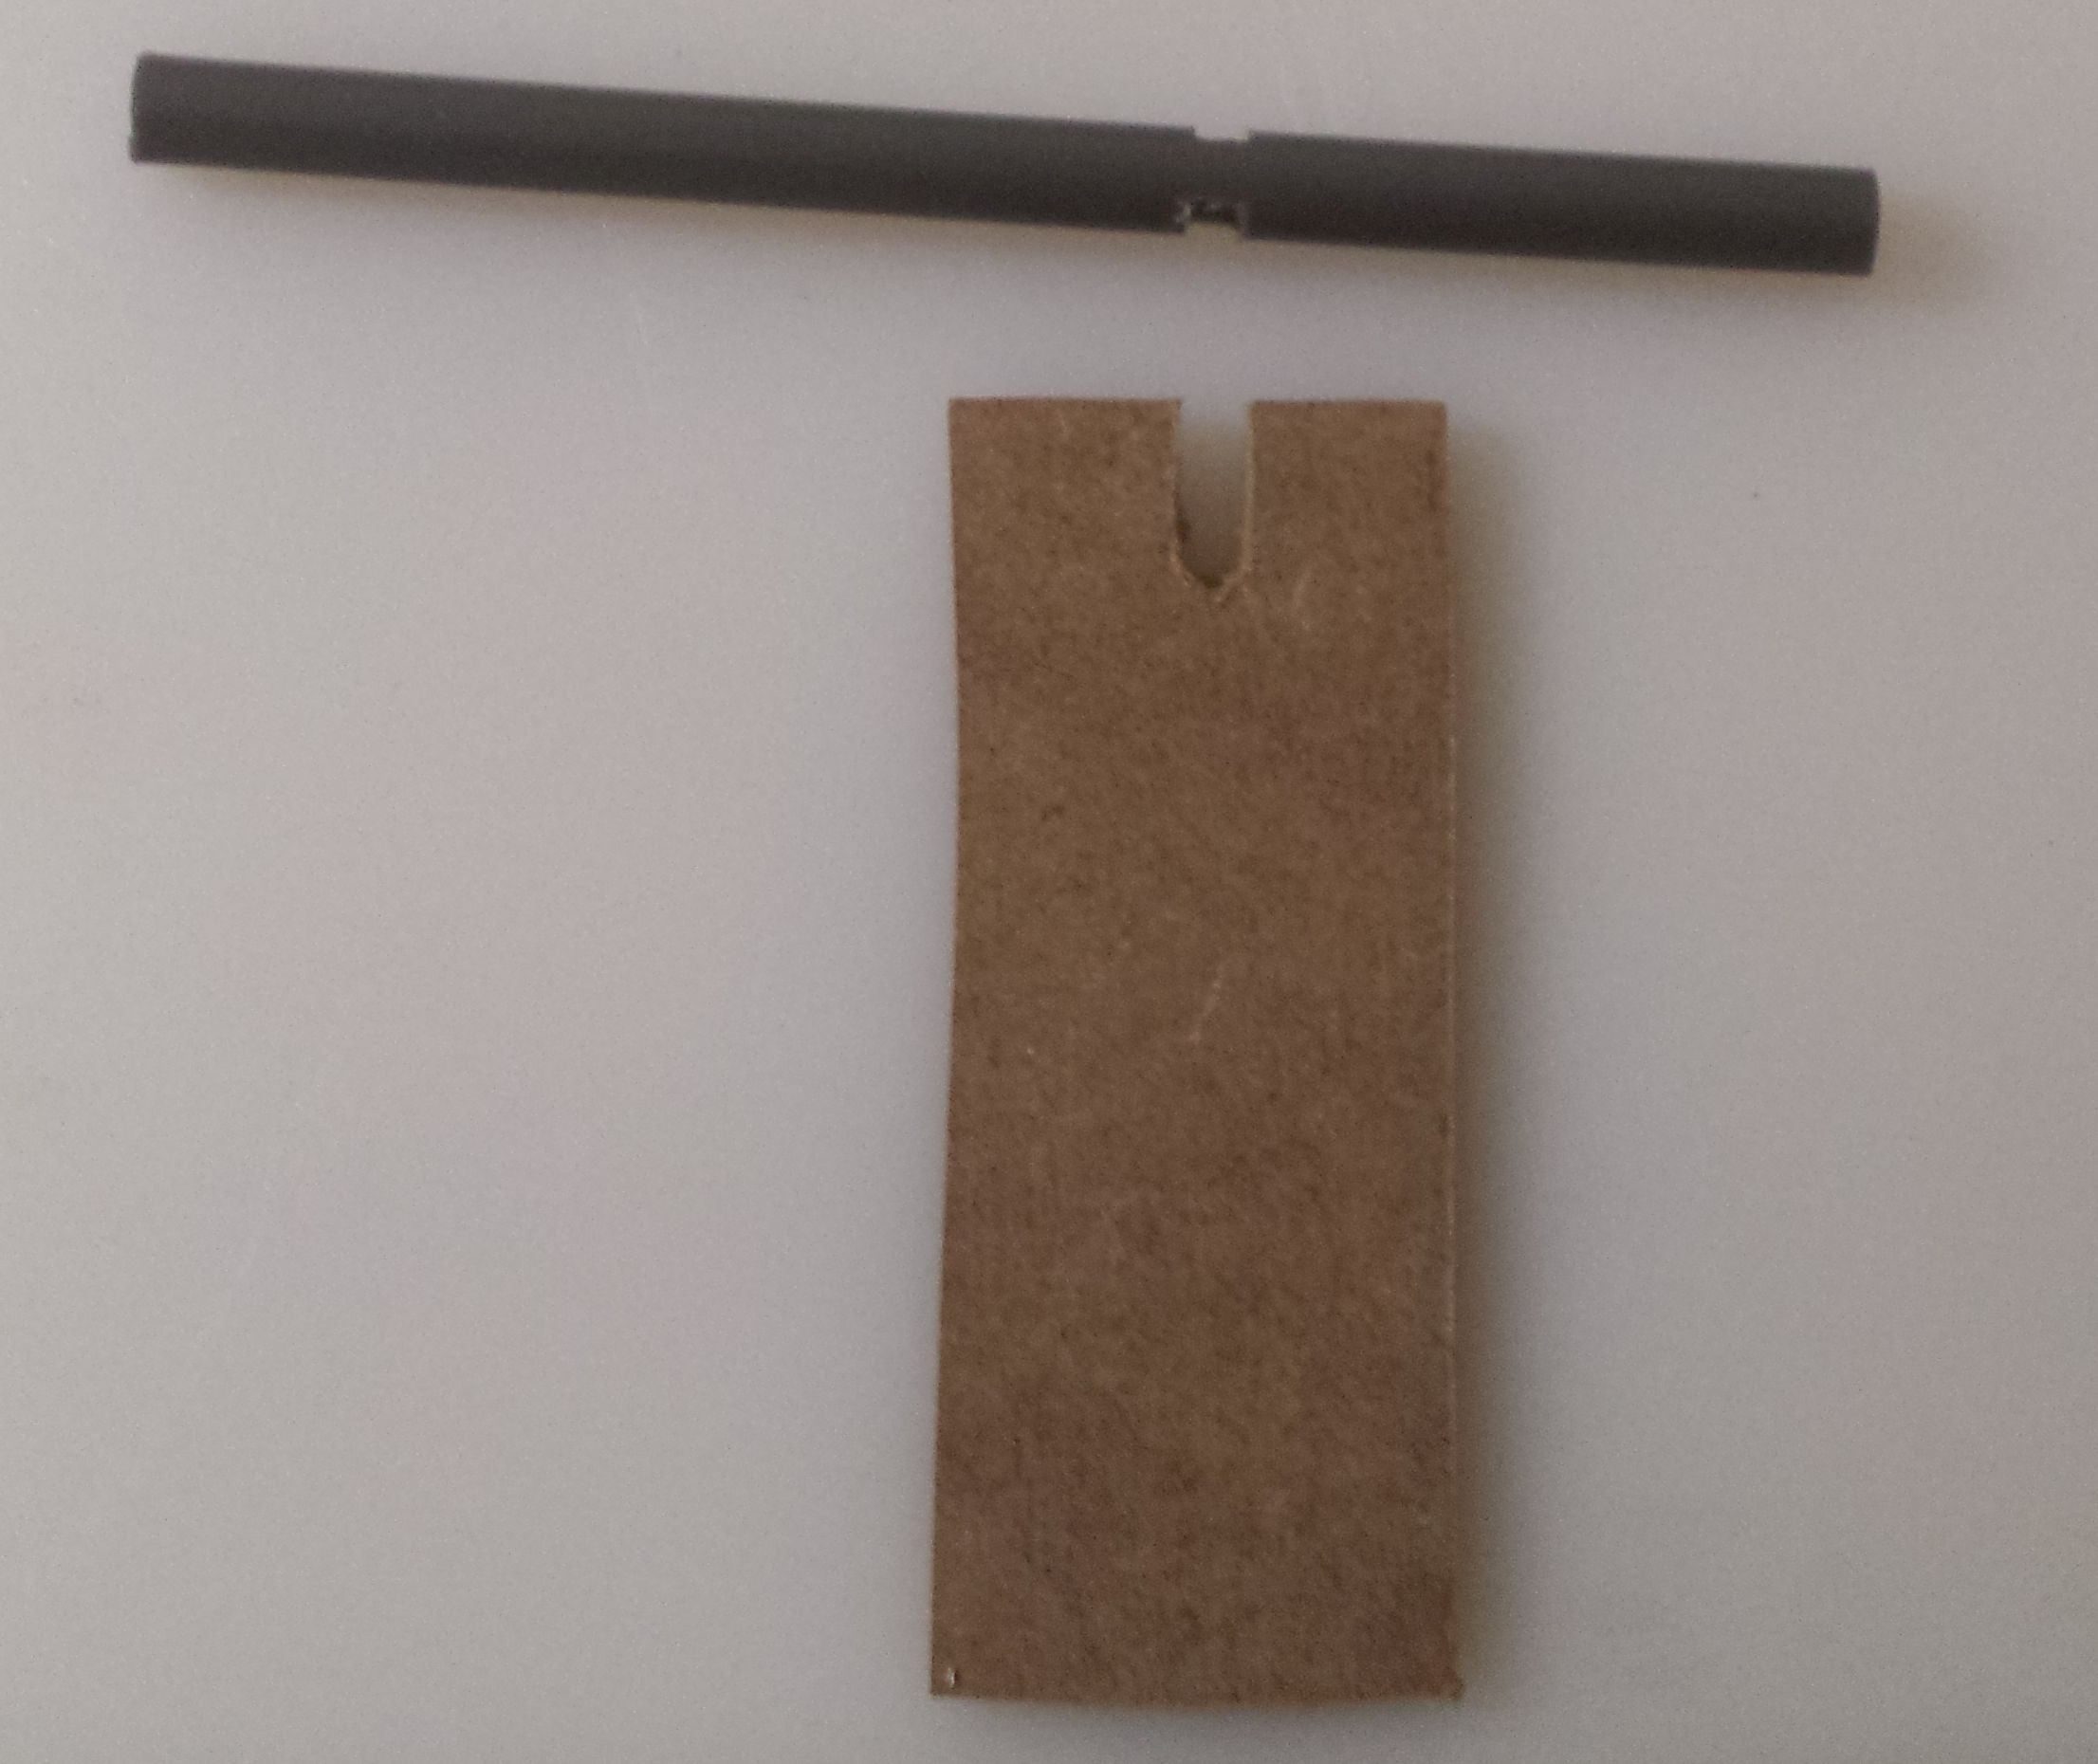
\includegraphics[height=55mm]{Bilder/koffer-adapter-einzeln}
								\caption{Einzelteile}
								\label{fig:koffer-adapter-einzeln}
							\end{subfigure}
							\hfill%
							\begin{subfigure}[t]{0.5\textwidth}
								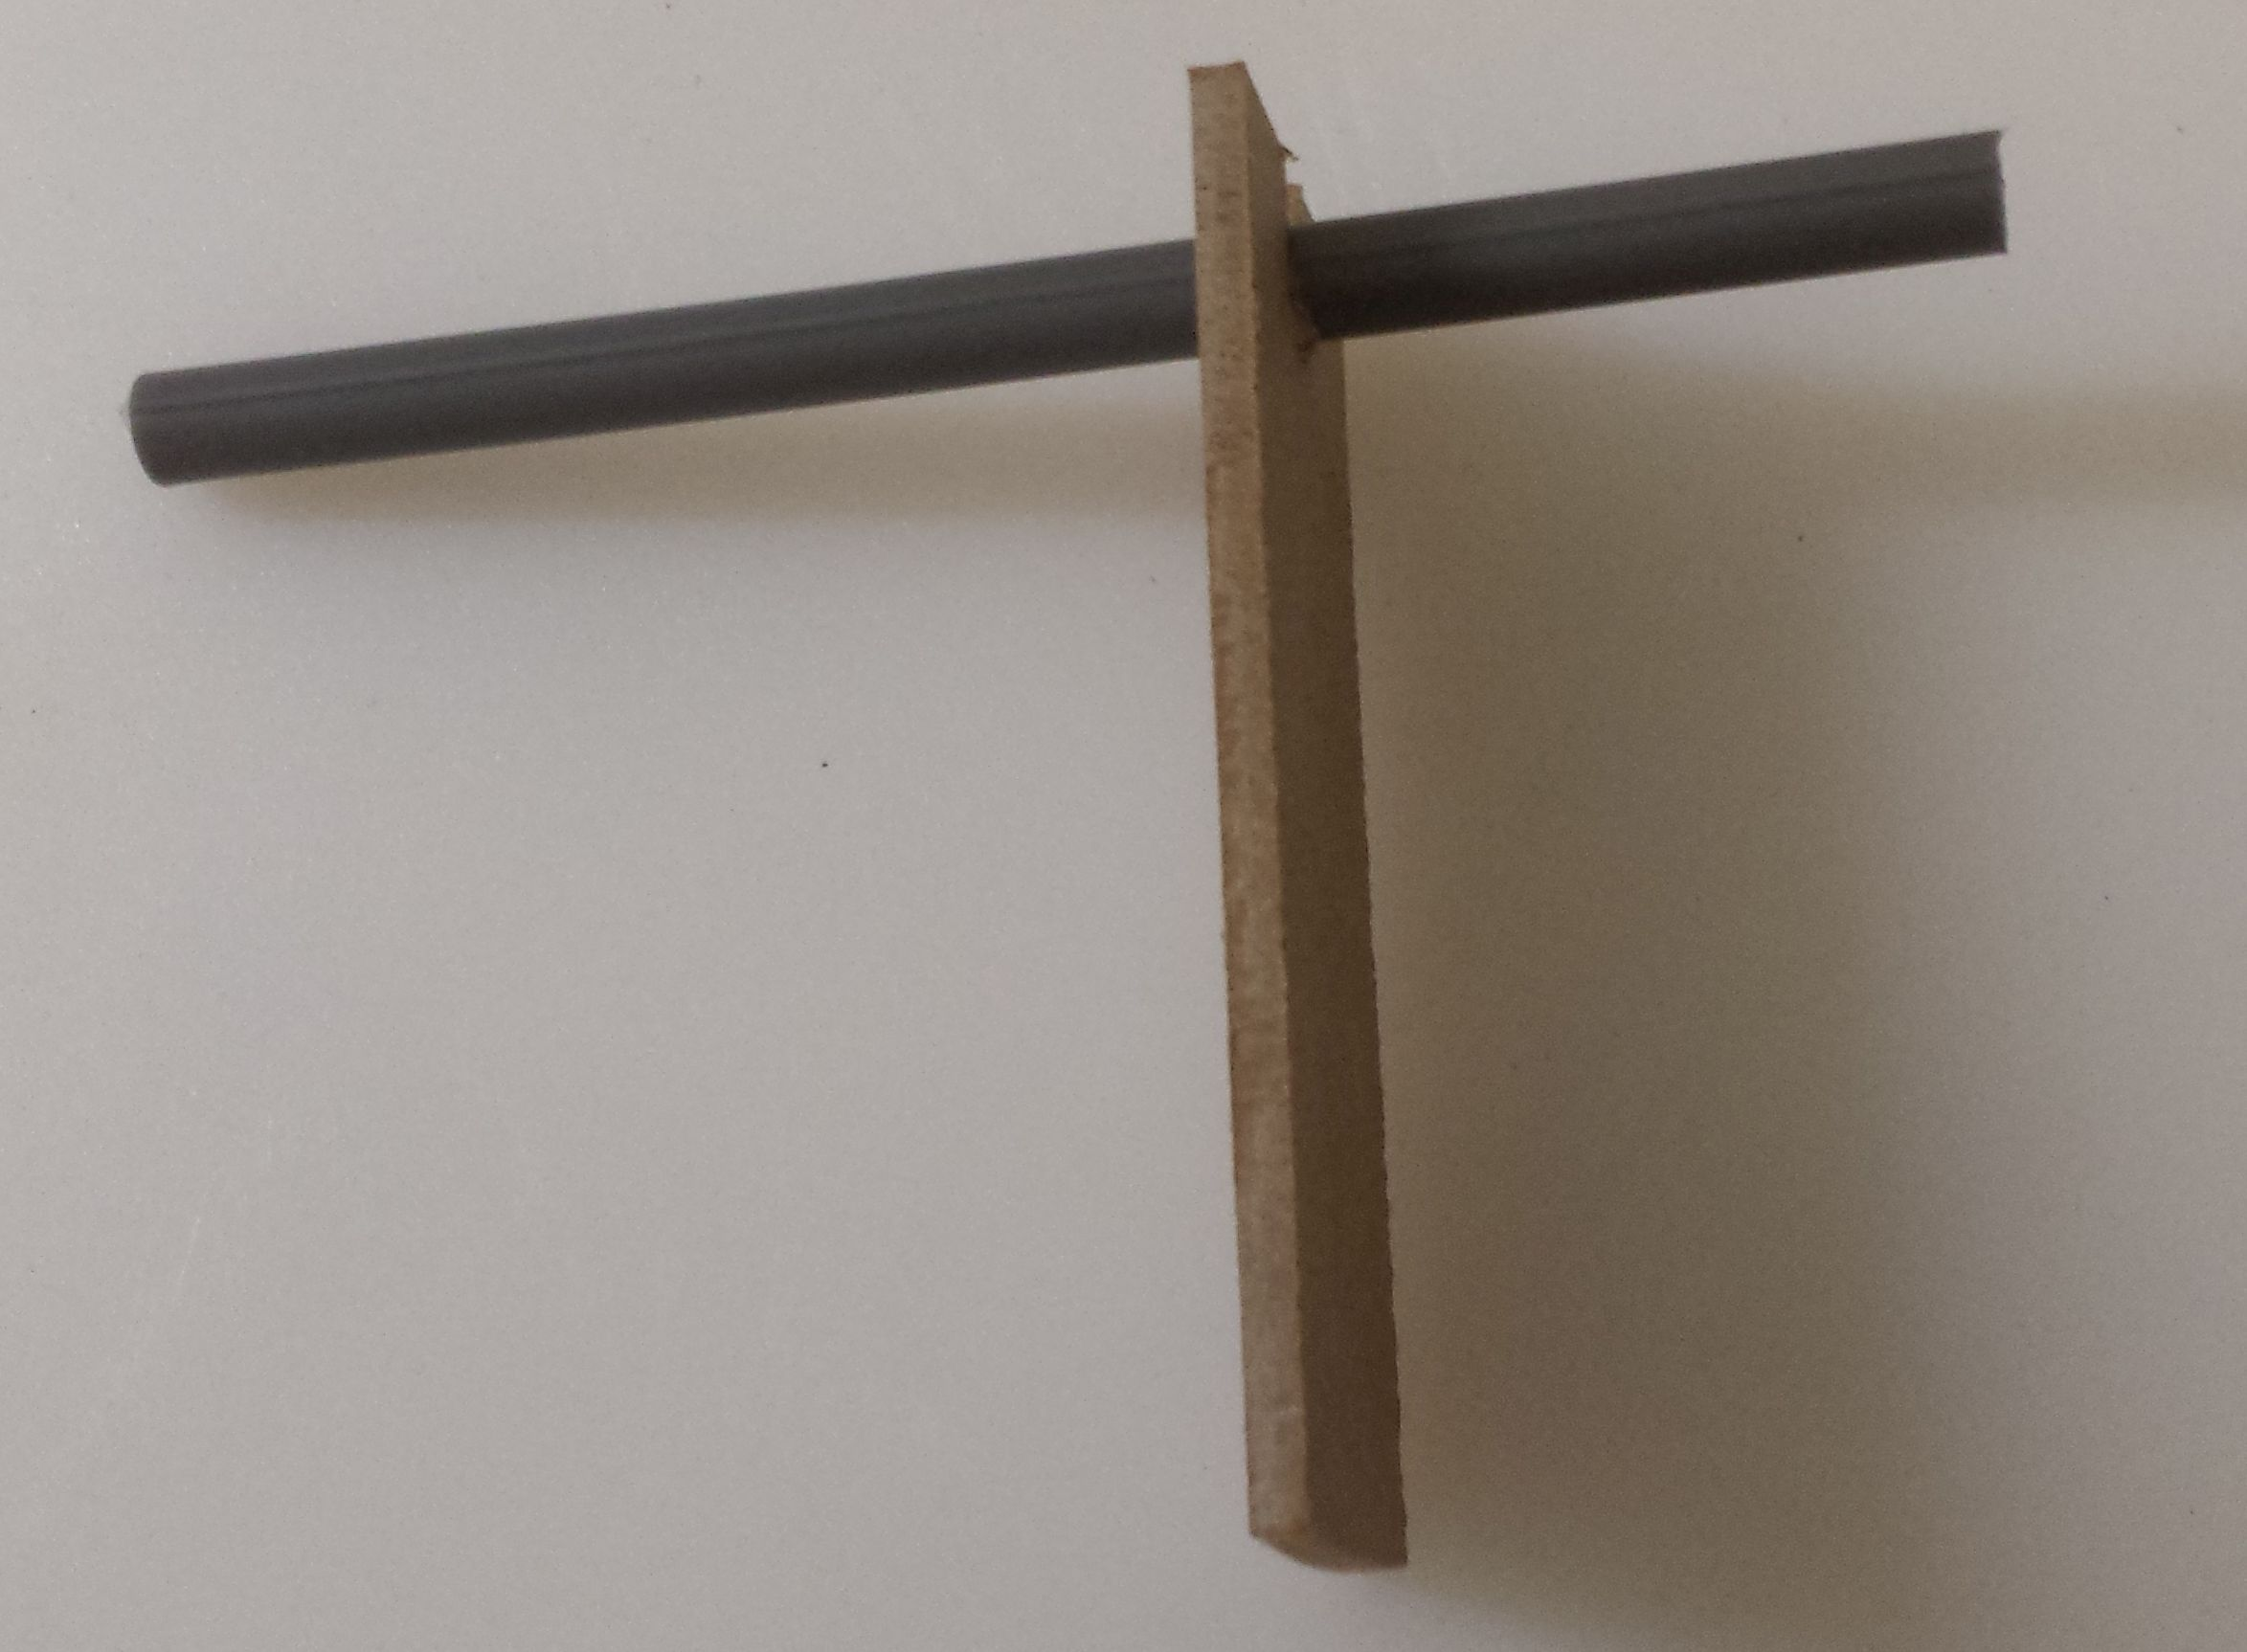
\includegraphics[height=55mm]{Bilder/koffer-adapter-zusammen}
								\caption{Zusammen}
								\label{fig:koffer-adapter-zusammen}
							\end{subfigure}
							%
							\caption{Antennenadapter}
						\end{figure}

						Nun muss das Antennenkabel durch das Rohr geführt werden, so dass der gewinkelte männliche SMA-Stecker an dem Ende des Rohrs liegt, welches näher an den Einschnitten liegt. Wird ein bereits fertig konfektioniertes Antennenkabel, z.\,B.\, das in der Materialliste aufgeführte, verwendet, muss das PVC-Rohr auf kompletter Länge aufgetrennt werden, um das Kabel einführen zu können. Konfektioniert man das Kabel selbst, kann die Buchse auf der Antennenseite nach dem Einfädeln angebracht werden, womit man sich das Auftrennen des Rohrs spart. Ist das Kabel durch das Rohr gefädelt und sind Winkelstecker und Buchse angebracht, sollte der gewinkelte Stecker kurz an der Box angeschraubt und der Adapter zusammengesteckt werden, damit man die nötige Länge für den Schrumpfschlauch zwischen MDF-Platte und Winkelstecker ausmessen kann. Dieser wird dann, nach Abschrauben des Winkelsteckers und Herausnehmen des Rohrs vom \enquote{Buchsenende} her aufgeschoben und erhitzt.

						Im nächsten Schritt muss das Rohr außerhalb des Koffers gebogen werden, damit die Antenne später senkrecht nach oben zeigt. Hierzu sollte das PVC-Rohr mit einem Heißluftföhn erwärmt und in größerem Radius (Koaxialkabel sollten nie geknickt werden!) gebogen werden.

						Zum Schluss wird die Antenne an die Buchse angeschraubt und die Verschraubung mit Schrumpfschlauch überdeckt. Die fertige Antenne, die außerhalb der Einsatzzeiten der Zündbox abgeschraubt im Koffer aufbewahrt werden kann, ist in Abbildung~\ref{fig:antennefertig} dargestellt.

						\begin{figure}
							\centering
							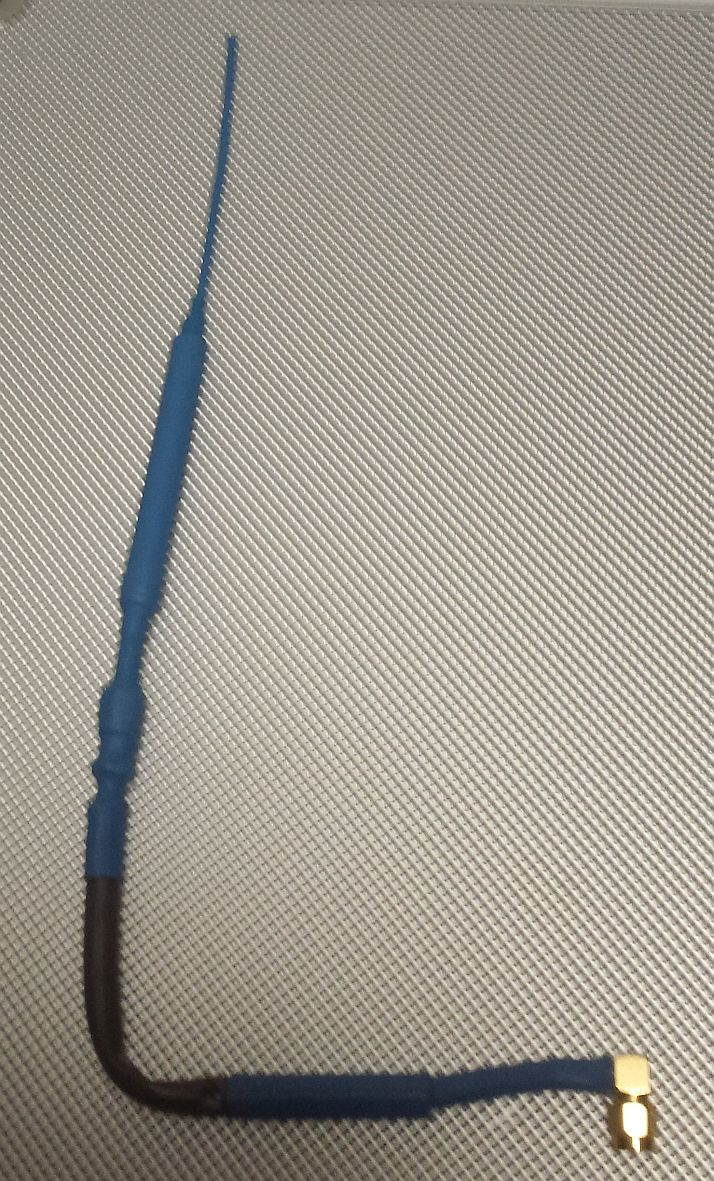
\includegraphics[]{Bilder/antennefertig}
							\caption{Einsatzbereite Antenne mit Zuleitung}
							\label{fig:antennefertig}
						\end{figure}

				\subsection{Gehäuse des Raspberry-Pi-Transmitters}

					tbd

		\chapter{Aufspielen des Bootloaders}
			\label{ch:bootloader}

			Bevor Firmwareupdates über die serielle Schnittstelle eingespielt werden können, muss zunächst ein Programm auf den Controller gespielt werden, dessen Aufgabe es ist, die eigentliche Firmware in den Speicher zu laden und zu starten. Dieses Programm ist der so genannte Bootloader, welcher beim Start des Devices für eine Sekunde überprüft, ob ein Firmwareupdate vorgenommen werden oder die {\anlage}-Firmware normal ausgeführt werden soll.

			\begin{figure}[!h]
				\centering
				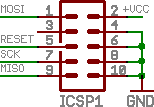
\includegraphics[width=.35\textwidth]{Bilder/isp}
				\caption{Pinbelegung des ISP-Platinensteckers: Ansicht von oben, Gehäuseaussparung an Pin~5. Quelle: \href{http://www.mikrocontroller.net}{\texttt{mikrocontroller.net}}}
				\label{fig:isp}
			\end{figure}

			Um den Bootloader auf den Controller zu brennen und einige Grundeinstellungen des Controllers, die so genannten Fuses, welche neben den Einstellungen, welche die Verwendung eines Bootloaders ermöglichen, auch Funktionen wie die Brown-Out-Detektion oder die Taktquelle regeln, wird ein spezielles Programmiergerät zur In-System-Programmierung (ISP) benötigt, welches den Controller in den Resetzustand versetzt und anschließend den Bootloader über die SPI-Schnittstelle an eine festgelegte Stelle im Flash-Speicher des Controllers schreibt.

			Auf der Platine jedes Devices ist für ISP ein zehnpoliger zweireihiger Wannenstecker vorgesehen, an den gängige Programmiergeräte wie der weit verbreitete \emph{AVRISP mkII} angeschlossen werden. Seine Pinbelegung ist in Abbildung~\ref{fig:isp} gezeigt. Nach einmaligem Flashen des Bootloaders und EEPROMs wird die ISP-Schnittstelle nicht wieder benötigt, alle weiteren Änderungen können über die serielle Schnittstelle und den Bootloader vorgenommen werden.

			\section{Verwendung des AVRISP mkII}

				Zum Brennen des Bootloaders gibt es ein Kommandozeilentool namens \emph{btldflsh.exe} für den \emph{AVRISP mkII}, welches auf \emph{AVRDUDE} basiert. Dem Tool muss als Parameter die iHex-Datei des controllertyp- und frequenzspezifischen Bootloaders übergeben werden.

				Für einen \texttt{ATmega328P} mit einer Taktfrequenz von \SI{9,8304}{\mega\hertz} lautet das Kommando:

				\begin{center}
					\emph{btldflsh.exe bootload\_m328p\_9830400.hex}
				\end{center}

				Die für {\anlage} benötigten Einstellungen für Fuses und die Datenübertragung werden auf diese Weise automatisch angepasst. Ebenfalls übertragen wird beim Flashen des Bootloaders eine Standardversion des EEPROMS, so dass die Devices standardmäßig 1 als Unique- und Slave-ID zugewiesen bekommen (Transmitter rekonfigurieren sich dann automatisch beim ersten Start der Firmware).

			\section{Verwendung eines anderen Programmieradapters}

				Selbstverständlich ist das Aufspielen des Bootloaders auch mit anderen Programmern möglich.

				Wichtig für die ordnungsgemäße Funktion des Bootloaders sowie später der Firmware ist neben einer fehlerfreien Programmierung auch das korrekte Setzen der Fuse-Bits, welches bei Einsatz eines alternativen Programmieradapters manuell vorgenommen werden muss.

				Für {\anlage} müssen die Fusebits beim \texttt{ATmega328P} gemäß Tabelle \ref{tab:fuses} gesetzt werden.

				\begin{table}[h]
					\centering
					\begin{tabularx}{.9\textwidth}{llX}
						\hline\hline
						\textbf{Fuse} & \textbf{Wert}     & \textbf{Bedeutung}                                                                                                                                                                             \\ \hline
						Low Fuse      & 0xF7              & Kein Taktteiler, kein Clock-Output, Ext. Full Swing Crystal als Taktquelle                                                                                                                     \\
						High Fuse     & 0xD6              & Reset-Pin nicht als I/O-Pin, kein Debug-Wire, SPI-Download erlaubt, Watchdog aus, EEPROM nicht löschen, Bootbereich~=~256~Wörter, Boot-Reset-Vektor aktiviert (=nach Reset Bootloader starten) \\
						Extended Fuse & 0x05\footnotemark & Brown-Out bei Versorgungsspannung unter $\SI{2,7}{\volt}$                                                                                                                                      \\ \hline\hline
					\end{tabularx}
					\caption{Fuse-Einstellungen beim \texttt{ATmega328P}}
					\label{tab:fuses}
				\end{table}
				\footnotetext{Bei der Extended Fuse werden nur die unteren drei Bit verwendet, die oberen fünf sind nicht in Gebrauch und können daher beliebig jeweils mit 1 oder 0 beschrieben und gelesen werden. Im Beispiel werden die nicht-relevanten Bits mit 0 beschrieben, so dass sich der Wert 0x05 ergibt, äquivalent dazu könnte der Wert aber beispielsweise auch 0xFD oder 0xA5 lauten.}

				Wird beim Flashen des Bootloaders das Standard-EEPROM-Image nicht mitübertragen, die herstellerseitige Voreinstellung des EEPROMs also nicht verändert, werden Zündboxen~-- nach dem Programmieren der \enquote{echten} Firmware~-- zunächst \enquote{E} bzw. \enquote{e} für \enquote{Error} als Unique- bzw. Slave-ID melden, da an den Speicherstellen für IDs und Prüfsummen nicht zueinander passende Werte stehen. Die Zündbox muss dann einmalig kabelgebunden über die lokale Konfiguration auf gültige Werte eingestellt werden.

		\chapter{Tipps und Tricks}

			\section[5V-LCD an 3,3V]{5\,V-LCD an 3,3\,V}

				Zwar gibt es inzwischen auch LCDs, welche sich von Haus aus für eine Versorgung mit $\SI{3,3}{\volt}$ eignen, viele Displays jedoch sind noch für $\SI{5}{\volt}$ ausgelegt. Der interne Controller funktioniert ohne Probleme auch bei geringerer Spannung, Knackpunkte sind jedoch die Kontrastspannung für das LCD sowie die Hintergrundbeleuchtung.

				Die Kontrastspannung wird zwischen Pin~2 und Pin~3 gemessen und ist verantwortlich für die Lesbarkeit der Schrift auf dem Display. Im \enquote{Normalfall}~-- also bei Betrieb des Displays mit einer Versorgungsspannung von $\SI{5}{\volt}$~-- wird Pin~3 auf $\SI{0}{\volt}$ gelegt, so dass sich eine Kontrastspannung von $\SI{5}{\volt}$ einstellt. Liegen an Pin~2 nur $\SI{3,3}{\volt}$ an, muss Pin~3 folglich mit einer negativen Spannung verbunden werden, um die nötige Kontrastspannung zu erreichen.

				Als Quelle der negativen Spannung dient der RS232-Treiberbaustein, der am Pin V- eine Spannung von $\SI{-5,5}{V}$ zur Verfügung stellt. Über einen Spannungsteiler~-- im Schaltplan auf Seite~\pageref{fig:transmitterschematic} von $R12 = \SI{3,3}{\kilo\ohm}$ und $R13 = \SI{6,8}{\kilo\ohm}$ gebildet~-- zwischen V- und GND wird daher Pin~3 des LCD auf $\SI{-1,8}{\volt}$ gelegt.

				Manche LCDs torpedieren diesen Versuch, indem Pin~3 relativ niederohmig mit GND verbunden wird. Man sollte also im abgeklemmten Zustand den Widerstand zwischen Pin 1 und Pin 3 messen und bei Bedarf den eventuell auf der LCD-Platine befindlichen Widerstand zwischen den beiden Pins auslöten.

				Die Hintergrundbeleuchtung wird über die Pins~15 und 16 versorgt. Zwischen diesen Pins befindet sich in Reihe zu den LEDs in aller Regel noch ein Widerstand, welcher den Strom durch die LEDs begrenzt und für eine Spannung von $\SI{5}{\volt}$ zwischen den Pins ausgelegt ist. Bei $\SI{3,3}{\volt}$ zwischen Pin~15~\&~16 erscheint das LCD daher möglicherweise zu dunkel, so dass man den Widerstand durch einen kleineren Wert ersetzen kann, um die Spannungsdifferenz auszugleichen.

				Der ursprüngliche LED-Vorwärtsstrom sowie die Aufteilung der Spannung auf LED und Vorwiderstand können durch Anlegen von $\SI{5}{\volt}$ zwischen Pin~15~\&~16, Spannungsmessung über dem Original-Widerstand und anschließende Division durch den Widerstandswert (korrekt ablesen oder messen) ermittelt werden. Da der Spannungsabfall über den LEDs sich nicht ändert und der Strom gleich bleiben soll, muss der Wert des neuen Widerstands so verkleinert werden, dass bei identischem Stromfluss über ihm $\SI{1,7}{\volt}$ weniger abfallen als am Original-Widerstand.

				Ist z.\,B. original ein Widerstand von $\SI{150}{\ohm}$ verbaut, über dem eine Spannung von $\SI{2}{\volt}$ anliegt (hieraus resultiert eine LED-Vorwärtsspannung von $\SI{3}{\volt}$), ergibt sich ein LED-Vorwärtsstrom von $\SI{13}{\milli\ampere}$. Dementsprechend wäre bei einem Spannungsabfall von nur noch $\SI{0,3}{\volt}$ für den gleichen Strom ein Widerstand von $\SI{22}{\ohm}$ einzusetzen.

			\section{Antennenbau}

				Antennen für die verwendete Übertragungsfrequenz von \SI{868}{\mega\hertz} gibt es in großer Auswahl zu kaufen, eine einfache, omnidirektionale Antenne, welche ein sehr gutes Stehwellenverhältnis von <1,3:1 erzielt, kann aber auch relativ schnell selbst gebaut werden. Auf möglichst exakte Einhaltung der Abmessungen ist dabei zu achten:
				\begin{itemize}
					\item Koaxialkabel RG316
					\item SMA-Steckverbinder (üblicherweise männliche Ausführung)
					\item Kupfer- oder Messingröhrchen mit 8\,mm Durchmesser und 66,5\,mm Länge
					\item Distanzhülse aus Kunststoff mit 5\,mm Länge, 7\,mm Außendurchmesser und 3,6\,mm Innendurchmesser
					\item Schrumpfschläuche mit 1,2\,mm, 2,4\,mm, 4,8\,mm und 9,5\,mm Durchmesser vor dem Schrumpfen
				\end{itemize}

				\begin{figure}
					\centering
					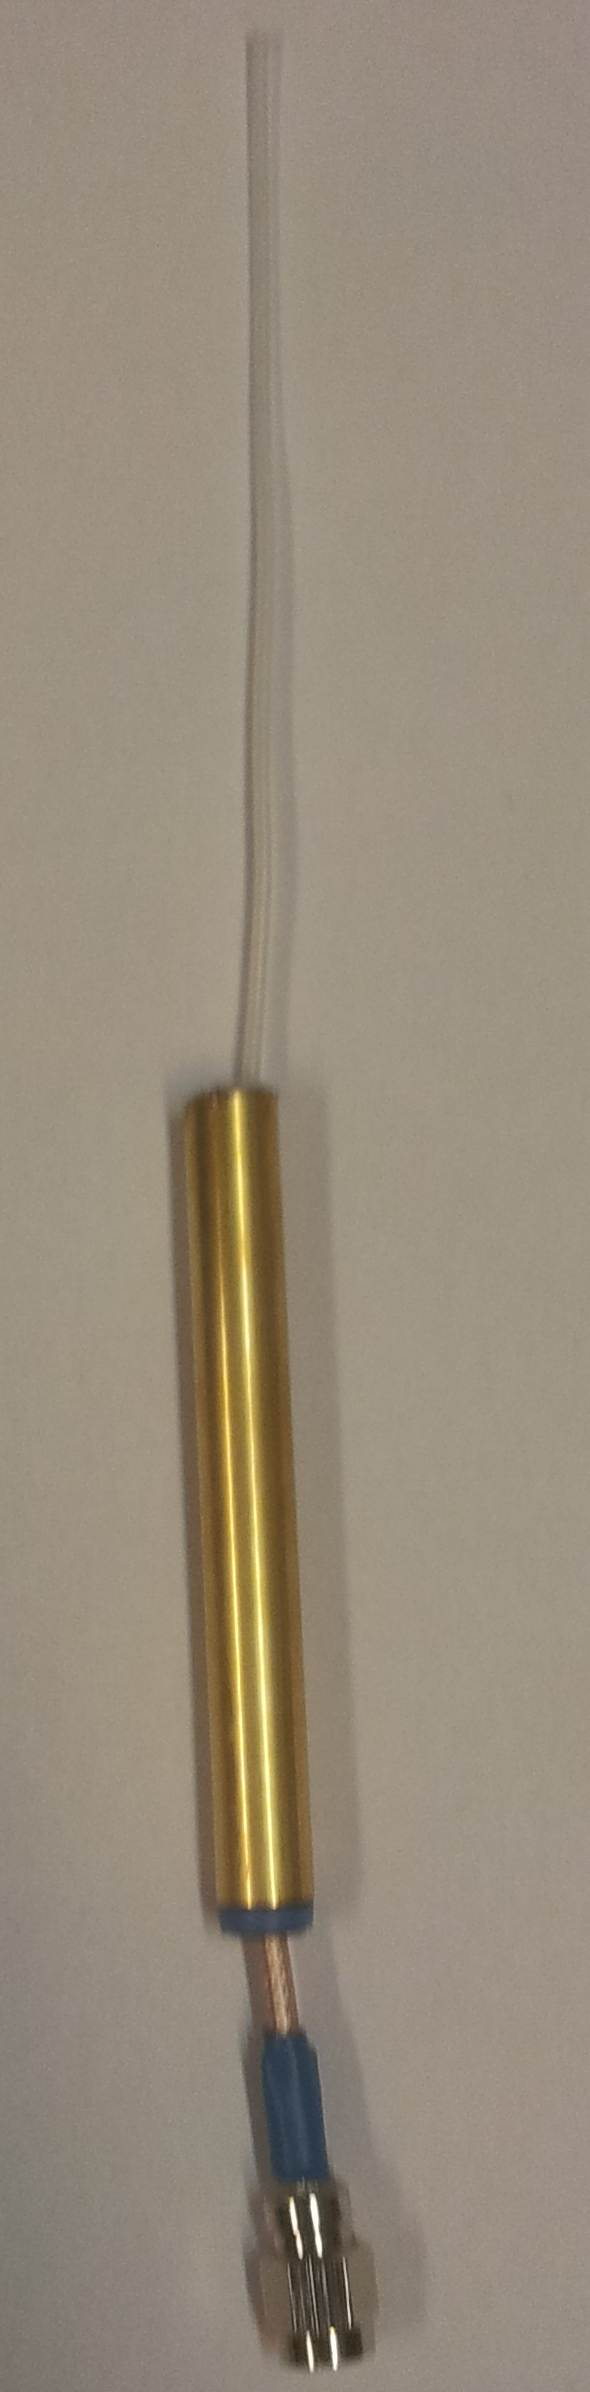
\includegraphics[height=10cm]{Bilder/Antenne}%
					\includegraphics[height=10cm]{Bilder/AntenneKomplett}
					\caption{Antenne ohne Schrumpfschlauch (links) und komplett fertig (rechts)}
					\label{fig:antenne}
				\end{figure}

				Die Antenne wird als Sperrtopfantenne bezeichnet und besitzt den in Abbildung~\ref{fig:antenne} gezeigten Aufbau. Der oberste Teil ist 88\,mm lang und besteht aus dem Innenleiter des Koaxialkabels mit dem ihn umgebenden Dielektrikum. Im mittleren Teil befindet sich ein 66,5\,mm langes Röhrchen, welches an seinem oberen Ende mit möglichst kurzer Verbindung an das Schirmgeflecht des Koaxialkabels angelötet wird. Anschließend folgt eine beliebige Länge Koaxialkabel, am Ende schließlich der Steckverbinder zum Anschluss an das Funkmodul.

				\begin{figure}[t]
					\centering
					\includegraphics[height=8cm]{Bilder/vswrmessung}%
					\caption{VSWR-Messung der gefertigten Antenne am Netzwerkanalysator}
					\label{fig:vswrmessung}
				\end{figure}

				Der Aufbau der Antenne erfolgt folgendermaßen:
				\begin{enumerate}
					\item Von der Rolle RG316 ein Stück der Länge abschneiden, welche später der Gesamtlänge von Antennenspitze bis zum Anschluss an das Funkmodul bzw. einen Adapterstecker entspricht
					\item Entfernung des Kunststoffmantels auf einer Länge von 88\,mm
					\item Entfernung des nun freiliegenden Schirmgeflechts auf einer Länge von 84\,mm, so dass noch 4\,mm des Schirmgeflechts verbleiben.
					\item Auftrennen und Verdrillen des Schirmgeflechts
					\item Verdicken des Koaxialkabels mit einem 10\,mm langen Stück Schrumpfschlauch, dessen Mitte 66,5\,mm vom oberen Ende der Ummantelung entfernt sein sollte.
					\item Aufschieben der Distanzhülse in die Mitte des soeben verstärkten Teils. Gegen Abrutschen nach unten ggf. mit weiterem Schrumpfschlauch unterhalb der Hülse sichern.
					\item Großzügiges Vorverzinnen des Röhrchens an einer Stelle der Innenwand
					\item Überstülpen des Röhrchens und Anlöten des verdrillten Schirmgeflechts an der Innenwand
					\item Gesamte Konstruktion mit Schrumpfschlauch stabilisieren (nach jedem Schritt schrumpfen!):
							\begin{enumerate}
								\item Ein 88\,mm langes Stück Schrumpfschlauch $1,2$ über den obersten Teil der Antenne
								\item Ein 90\,mm langes Stück Schrumpfschlauch $2,4$ über den obersten Teil der Antenne, unmittelbar nach dem Schrumpfen die noch heißen oben überstehenden 2\,mm Schlauch durch Zusammendrücken verschmelzen
								\item Ein 2,5\,mm langes Stück Schrumpfschlauch $9,5$ über den aus dem Röhrchen herausstehenden Teil der Distanzhülse
								\item Ein 80\,mm langes Stück Schrumpfschlauch 9,5 über Röhrchen und Distanzhülse, so dass auf beiden Seiten etwa 5\,mm überstehen
								\item Mit einem 10\,mm langen Stück Schrumpfschlauch $4,8$ den Übergang zwischen oberem Antennenteil und Röhrchen versiegeln
							\end{enumerate}
					\item Falls nötig: Kabel in Endposition einfädeln, bevor SMA-Steckverbinder am intakten Ende angebracht wird
				\end{enumerate}

				Um den SMA-Steckverbinder anzubringen, müssen vom intakten Ende aus gemessen zunächst \SI{12}{\milli\metre} des Mantels entfernt werden, anschließend \SI{8}{\milli\metre} des Schirmgeflechts und zuletzt auch \SI{4}{\milli\metre} des Dielektrikums. Nun werden Schrumpfschlauch und Crimpröhrchen auf das Kabel geschoben, anschließend der kleine Stecker am Innenleiter angelötet. Das Schirmgeflecht wird aufgefächert, das Gehäuse aufs Kabel geschoben und das Crimpröhrchen aufgesteckt, vercrimpt und Schrumpfschlauch darüber angebracht. Wenn gewünscht kann~-- wie in~\ref{fig:antenne} rechts zu sehen~-- Schrumpfschlauch 9,5 als Witterungsschutz über dem gesamten Steckverbinder angebracht werden.

				Die in Abbildung~\ref{fig:vswrmessung} dargestellte Messung am Netzwerkanalysator zeigt eine sehr gute Anpassung dieser Antenne an \SI{50}{\ohm} im Bereich um \SI{868}{\mega\hertz}.

			\section{Kompilieren der Firmware}

				Falls keine der im Repository zur Verfügung gestellten Hex-Files verwendet werden soll, besteht auch die Möglichkeit, seine eigene Firmware aus den Quellcodedateien zu kompilieren. Hierfür wird der die AVR-GCC-Toolchain benötigt, welche es für Windows z.\,B. als fertiges Paket \texttt{WinAVR\footnote{Download \href{http://sourceforge.net/projects/winavr/files/}{WinAVR}}} gibt.

				\texttt{WinAVR} entspricht leider schon länger nicht mehr dem aktuellen Stand des GCC-Compilers, man kann entweder bei Atmel\footnote{Download \href{http://www.atmel.com/tools/ATMELAVRTOOLCHAINFORWINDOWS.aspx}{Atmel-Toolchain} (kostenlose Registrierung notwendig)} oder bei im Sourceforge-Repository%
				\footnote{Downloadlink: \href{http://sourceforge.net/projects/mobilechessboar/files}{Sourceforge}} von Georg-Johann Lay aktuellere Versionen ziehen und diese über die alten \texttt{WinAVR}-Verzeichnisse kopieren.

				Anschließend ist darauf zu achten, dass das Unterverzeichnis \enquote{bin} in der PATH-Variable hinterlegt ist, so dass man die dort befindlichen Anwendungen aus jedem anderen Ordner unmittelbar aufrufen kann.

				Der Herstellungsprozess gliedert sich in folgende Schritte:
				\begin{enumerate}
					\item Kompilieren der Quellcodedateien (.c) in noch nicht gelinkte Dateien (.o)
					\item Linken zu einer Gesamtdatei (.elf)
					\item Umwandeln in eine Hexdatei (.hex), welche mit dem Bootloader über die serielle Schnittstelle auf den Controller geschrieben werden kann
				\end{enumerate}

				Der gesamte Ablauf kann transparent in der Datei \enquote{build\_hexfiles.bat} im Verzeichnis \enquote{Hexfiles} nachvollzogen werden.

			\section{Umrechnung zwischen Watt und dBm}
				Die Umrechnung zwischen den Einheiten Watt (linear) und dBm (logarithmisch) erfolgt nach folgenden Formeln:

				\begin{center}
					\begin{tabularx}{.6\textwidth}{c@{ $\rightarrow$ }c@{ :\hspace*{1cm}}c@{ = }X}
						$\si{\dBm}$  & $\si{W}$    & $P_\text{W}$   & $10^{\left(\frac{P_\text{dBm}}{10}-3\right)}$                                      \\[12pt]
						$\si{\watt}$ & $\si{\dBm}$ & $P_\text{dBm}$ & $10 {\cdot} \log_{10}\left( \frac{1000 {\cdot} P_\text{W}}{\SI{1}{\watt}} \right)$ \\
					\end{tabularx}
				\end{center}

				Anhand der Formeln wird klar, dass die maximale Sendeleistung des \texttt{RFM69CW} 1250-mal höher als die Minimalleistung liegt: $\SI{-18}{\dBm}$ entsprechen $\SI{16}{\micro\watt}$, $\SI{13}{\dBm}$ hingegen $\SI{20}{\milli\watt}$.

				Addition und Subtraktion in der logarithmischen Einheit sind gleichbedeutend mit Multiplikation bzw. Division in der linearen. Erhöht (verringert) sich die Leistung um $\SI{3}{\decibel}$, verdoppelt (halbiert) sie sich im linearen Maßstab. Addition bzw. Subtraktion um $\SI{10}{\decibel}$ bedeuten eine Multiplikation mit bzw. Division durch 10.

				\bookmarksetup{startatroot}
				\addtocontents{toc}{\bigskip}
				\listoffigures
				\listoftables

		\chapter*{Danksagung}%
			\addcontentsline{toc}{chapter}{Danksagung}

			Vielen Dank an alle, die in irgendeiner Form zur Entwicklung und Verbesserung von {\anlage} beigetragen haben!

			Ein ganz spezielles Dankeschön an:
			\begin{itemize}
				\item Marc Weissmann, der mit ursprünglich seinem, mittlerweile unserem gemeinsamen Projekt \href{http://www.facebook.com/FIREErlangen}{\texttt{FIRE~-- Feuerwerk im Röthel\-heim\-park Er\-langen}} den Ansporn zu dieser Entwicklung gegeben und ihr von Beginn an trotz einiger mittlerweile behobener \enquote{Kinderkrankheiten} immer voll vertraut hat. Videos unserer bisherigen mit {\anlage} geschossenen Feuerwerke:
						\begin{itemize}
							\item[*] \underline{\href{https://vimeo.com/116115628}{Silvesterfeuerwerk 2014/15}}
							\item[*] \underline{\href{https://vimeo.com/150594996}{Silvesterfeuerwerk 2015/16}}
							\item[*] \underline{\href{https://vimeo.com/198168273}{Silvesterfeuerwerk 2016/17}}
							\item[*] \underline{\href{https://www.youtube.com/watch?v=uPTW1dpsVoU}{Hochzeitsfeuerwerk 2017}}
						\end{itemize}
				\item Das gesamte private Umfeld, das die Arbeit am Projekt stets mit Fassung getragen und mit Interesse verfolgt hat.
				\item Jens Nachtigal, dem Hauptprogrammierer und Anstoßgeber zur Entwicklung des Raspberry-Pi-Transmitters.
				\item Die \enquote{Nachbau-Pioniere} Matthias Pee und Cedrik Sikora für Ideen und wertvolle Hinweise.
				\item \href{http://www.mikrocontroller.net}{\texttt{mikrocontroller.net}} für Hilfe in Sachen Hardware und Programmierung.
				\item \href{http://www.feuerwerk-forum.de}{\texttt{feuerwerk-forum.de}} für Erklärungen zum Thema elektrische Zündung und natürlich die Zündsoftware {\pic} von User \emph{pyrobla}.
				\item \href{http://www.saleae.com}{\texttt{Saleae}} für den grandiosen Logic 8, der wertvolle Dienste zur Erschließung des \texttt{RFM69} geleistet hat.
				\item Der \texttt{Brauerei Loscher} für Club Mate, den Bastler-Treibstoff.
				\item Die vielen tollen Open-Source- und Freeware-Lösungen, welche die Softwareentwicklung erst möglich gemacht haben:
						\begin{itemize}
							\item Die GCC-Community für die \texttt{AVR-GCC-Toolchain} zum Programmieren des Mikrocontrollers.
							\item Die Eclipse-Foundation für die Programmierumgebung \texttt{Eclipse}, Kees Bakker und Thomas Holland für die Erweiterung \texttt{AVREclipse} sowie Ben Gardner für \texttt{Uncrustify} und die damit verbundene Übersichtlichkeit des Quellcodes.
							\item Peter Dannegger für den robusten, aber dennoch schlanken Bootloader \texttt{FastBoot}.
							\item Leo-Andres Hofmann für die schöne Windows-Oberfläche \texttt{UpdateLoader}.
							\item \texttt{Subversion} und \texttt{TortoiseSVN} bzw. \texttt{Git} und \texttt{GitHub} für die unkomplizierte Versionsverwaltung.
							\item {\LaTeX} und \texttt{TeXstudio} zur Erstellung des Handbuchs.
						\end{itemize}
			\end{itemize}

\end{document}
